\documentclass[hidelinks,a4paper,11pt,oneside,openany]{jsbook}

\usepackage{amsmath,amssymb}
\usepackage{bm}
\usepackage{graphicx}
\usepackage{subfigure}
\usepackage{verbatim}
\usepackage{wrapfig}
\usepackage{ascmac}
\usepackage{makeidx}

%\usepackage{titlesec}
%\setcounter{secnumdepth}{4}

\usepackage[acronym]{glossaries}
%\usepackage{glossaries}
\makeglossaries
%\newacronym{oss}{OSS}{Open Source Software}
\newacronym{sil2linuxmp}{SIL2LinuxMP}{OSADL's functional safety project}
\newacronym{hiics}{HiICS}{Hitachi Industry \& Control Solutions, Ltd.}
\newacronym{hil}{HIL}{Hitachi India Laboratory}
\newacronym{osadl}{OSADL}{Open Source Automation Development Lab}
\newacronym{ot}{OpenTech}{}
\newacronym{tuv}{TUeV Rheinland}{a certification authority}
\newacronym{linux}{Linux}{Linux Operating System}
\newacronym{iec61508}{IEC61508}{an unmrella functional safety stadard}
\newacronym{gnu}{GNU}{GNU's Not Unix!}
\newacronym{iso26262}{ISO26262}{a functional safety standard for vehicle}
\newacronym{inria}{INRIA}{French Institute for Research in Computer Science and Automation}
\newacronym{fp}{False-Positive}{False Positive Alerm}
\newacronym{android}{Android}{Android Operatin System}
\newacronym{git}{Git}{Git version control system}
\newacronym{cocci}{Coccinelle}{Coccinelle}
\newacronym{sm}{Semantic Patch}{Semantic Patch}
\newacronym{ocaml}{OCaml}{OCaml}
\newacronym{rg}{Regular Expression}{Regular Expression}
\newacronym{sed}{sed}{Stream Editor}
\newacronym{csmith}{Csmith}{Csmith}
\newacronym{gcc}{GCC}{GNU Compiler Collection}
\newacronym{llvm}{LLVM}{}
\newacronym{klee}{KLEE}{}
\newacronym{se}{Symbolic Execution}{}
\newacronym{bb}{BusyBox}{}
\newacronym{cpa}{CPAChecker}{}
\newacronym{cfa}{Control Flow Automaton}{}
\newacronym{gt}{GoogleTest}{}
\newacronym{art}{Abstract Reachability Tree}{}
\newacronym{aprove}{AProVE}{Automated Program Verification Environment}
\newacronym{cv}{CodeViz}{}
\newacronym{cflow}{cflow}{}
\newacronym{sv}{SV-COMP}{Competition on Software Verification}
\newacronym{gv}{GraphViz}{}
\newacronym{hero}{Herodotos}{}
\newacronym{pre}{Prequel}{}
\newacronym{gsn}{GSN}{Goal Structuring Notation}
\newacronym{ogsn}{OGSN}{OSADL GSN Editor}
\newacronym{eclipse}{Eclipse}{}
\newacronym{java}{Java}{}
\newacronym{dcase}{DCASE}{}
\newacronym{acedit}{ACEdit}{Assurance Case Editor}
\newacronym{advocate}{AdvoCATE}{}
\newacronym{py}{Python}{}
\newacronym{rmtoo}{rmToo}{Requirement Management Tool}
\newacronym{gui}{GUI}{Graphical User Interface}
\newacronym{srs}{SRS}{System Requirement Specification}
\newacronym{cui}{CUI}{Character User Interface}
\newacronym{gh}{GitHub}{}
\newacronym{syzkaller}{syzkaller}{}
\newacronym{fuzzer}{fuzzer}{}
\newacronym{qemu}{QEMU}{}
\newacronym{bugspot}{bugspot}{}
\newacronym{sil2}{SIL2}{Safety Integrity Level 2}
\newacronym{sil0}{SIL0}{Safety Integrity Level 0}
\newacronym{hr}{HR}{Highly Recommended}
\newacronym{r}{R}{Recommended}
\newacronym{rb}{Ruby}{}
\newacronym{ltp}{LTP}{Linux Test Project}
\newacronym{posix}{POSIX test suite}{}
\newacronym{black}{Black Box}{}
\newacronym{db4sil2}{DB4SIL2}{Database for SIL2}
\newacronym{gb}{GrayBox}{}
\newacronym{ftrace}{ftrace}{Function Tracer}
\newacronym{lopa}{LOPA}{Layer of Protection Analysis}
\newacronym{qm}{QM}{Quality Management}
\newacronym{glibc}{glibc}{GNU C Library}
\newacronym{cgroups}{cgroups}{Control Groups}
\newacronym{seccomp}{seccomp}{Secure Computing Mode}
\newacronym{ccf}{CCF}{Common Cause Failure}
\newacronym{dvd}{Live-DVD}{}
\newacronym{dl}{Debian Live}{}
\newacronym{deb}{Debian}{}
\newacronym{ccb}{CCB}{Change Control Board}
\newacronym{gitstats}{GitStats}{git history statistics generator}
\newacronym{codemini}{Code Minimization}{}
\newacronym{hub}{GitHub}{}
\newacronym{overflow}{Stack Overflow}{}
\newacronym{sparse}{sparse}{}
\newacronym{comp}{Complexity}{}
\newacronym{mc}{McCabe}{}
\newacronym{sc}{Safety Critical}{}
\newacronym{cr}{Compliance Route}{}
\newacronym{adas}{ADAS}{Advanced Driving Assistant System}
\newacronym{hazop}{HAZOP}{Hazard and Operability Studies}
\newacronym{irc}{IRC}{Internet Relay Chat}
\newacronym{atc}{ATC}{Acceptance and Test Criteria}
\newacronym{yocto}{Yocto Project}{}
\newacronym{agl}{AGL}{Automotive Grade Linux}
\newacronym{genivi}{GENIVI Alliance}{}
\newacronym{wtc}{World Trade Center}{World Trade Center Bangalore}
\newacronym{ama}{Amazon}{}
\newacronym{kslta}{KSLTA}{}
\newacronym{toast}{Toastmasters Club}{人生道場 Toastmasters Club}{}
\newacronym{toastint}{Toastmasters International}{}
\newacronym{ir}{IR}{Indian Railways}
\newacronym{rac}{RAC}{Reservation Against Cancellatio}
\newacronym{wl}{Waiting List}{}
\newacronym{maketrip}{MakeMyTrip}{}
%\newacronym{}{}{}
%\newacronym{}{}{}
%\newacronym{}{}{}
%\newacronym{}{}{}
%\newacronym{}{}{}
%\newacronym{}{}{}
%\newacronym{}{}{}


\newacronym{oss}{OSS}{Open Source Software}
\newacronym{sil2linuxmp}{SIL2LinuxMP}{OSADL's functional safety project}
\newacronym{hiics}{HiICS}{Hitachi Industry \& Control Solutions, Ltd.}
\newacronym{hil}{HIL}{Hitachi India Laboratory}
\newacronym{osadl}{OSADL}{Open Source Automation Development Lab}
\newacronym{ot}{OpenTech}{}
\newacronym{tuv}{TUeV Rheinland}{a certification authority}
\newacronym{linux}{Linux}{Linux Operating System}
\newacronym{iec61508}{IEC61508}{an unmrella functional safety stadard}
\newacronym{gnu}{GNU}{GNU's Not Unix!}
\newacronym{iso26262}{ISO26262}{a functional safety standard for vehicle}
\newacronym{inria}{INRIA}{French Institute for Research in Computer Science and Automation}
\newacronym{fp}{False-Positive}{False Positive Alerm}
\newacronym{android}{Android}{Android Operatin System}
\newacronym{git}{Git}{Git version control system}
\newacronym{cocci}{Coccinelle}{Coccinelle}
\newacronym{sm}{Semantic Patch}{Semantic Patch}
\newacronym{ocaml}{OCaml}{OCaml}
\newacronym{rg}{Regular Expression}{Regular Expression}
\newacronym{sed}{sed}{Stream Editor}
\newacronym{csmith}{Csmith}{Csmith}
\newacronym{gcc}{GCC}{GNU Compiler Collection}
\newacronym{llvm}{LLVM}{}
\newacronym{klee}{KLEE}{}
\newacronym{se}{Symbolic Execution}{}
\newacronym{bb}{BusyBox}{}
\newacronym{cpa}{CPAChecker}{}
\newacronym{cfa}{Control Flow Automaton}{}
\newacronym{gt}{GoogleTest}{}
\newacronym{art}{Abstract Reachability Tree}{}
\newacronym{aprove}{AProVE}{Automated Program Verification Environment}
\newacronym{cv}{CodeViz}{}
\newacronym{cflow}{cflow}{}
\newacronym{sv}{SV-COMP}{Competition on Software Verification}
\newacronym{gv}{GraphViz}{}
\newacronym{hero}{Herodotos}{}
\newacronym{pre}{Prequel}{}
\newacronym{gsn}{GSN}{Goal Structuring Notation}
\newacronym{ogsn}{OGSN}{OSADL GSN Editor}
\newacronym{eclipse}{Eclipse}{}
\newacronym{java}{Java}{}
\newacronym{dcase}{DCASE}{}
\newacronym{acedit}{ACEdit}{Assurance Case Editor}
\newacronym{advocate}{AdvoCATE}{}
\newacronym{py}{Python}{}
\newacronym{rmtoo}{rmToo}{Requirement Management Tool}
\newacronym{gui}{GUI}{Graphical User Interface}
\newacronym{srs}{SRS}{System Requirement Specification}
\newacronym{cui}{CUI}{Character User Interface}
\newacronym{gh}{GitHub}{}
\newacronym{syzkaller}{syzkaller}{}
\newacronym{fuzzer}{fuzzer}{}
\newacronym{qemu}{QEMU}{}
\newacronym{bugspot}{bugspot}{}
\newacronym{sil2}{SIL2}{Safety Integrity Level 2}
\newacronym{sil0}{SIL0}{Safety Integrity Level 0}
\newacronym{hr}{HR}{Highly Recommended}
\newacronym{r}{R}{Recommended}
\newacronym{rb}{Ruby}{}
\newacronym{ltp}{LTP}{Linux Test Project}
\newacronym{posix}{POSIX test suite}{}
\newacronym{black}{Black Box}{}
\newacronym{db4sil2}{DB4SIL2}{Database for SIL2}
\newacronym{gb}{GrayBox}{}
\newacronym{ftrace}{ftrace}{Function Tracer}
\newacronym{lopa}{LOPA}{Layer of Protection Analysis}
\newacronym{qm}{QM}{Quality Management}
\newacronym{glibc}{glibc}{GNU C Library}
\newacronym{cgroups}{cgroups}{Control Groups}
\newacronym{seccomp}{seccomp}{Secure Computing Mode}
\newacronym{ccf}{CCF}{Common Cause Failure}
\newacronym{dvd}{Live-DVD}{}
\newacronym{dl}{Debian Live}{}
\newacronym{deb}{Debian}{}
\newacronym{ccb}{CCB}{Change Control Board}
\newacronym{gitstats}{GitStats}{git history statistics generator}
\newacronym{codemini}{Code Minimization}{}
\newacronym{hub}{GitHub}{}
\newacronym{overflow}{Stack Overflow}{}
\newacronym{sparse}{sparse}{}
\newacronym{comp}{Complexity}{}
\newacronym{mc}{McCabe}{}
\newacronym{sc}{Safety Critical}{}
\newacronym{cr}{Compliance Route}{}
\newacronym{adas}{ADAS}{Advanced Driving Assistant System}
\newacronym{hazop}{HAZOP}{Hazard and Operability Studies}
\newacronym{irc}{IRC}{Internet Relay Chat}
\newacronym{atc}{ATC}{Acceptance and Test Criteria}
\newacronym{yocto}{Yocto Project}{}
\newacronym{agl}{AGL}{Automotive Grade Linux}
\newacronym{genivi}{GENIVI Alliance}{}
\newacronym{wtc}{World Trade Center}{World Trade Center Bangalore}
\newacronym{ama}{Amazon}{}
\newacronym{kslta}{KSLTA}{}
\newacronym{toast}{Toastmasters Club}{人生道場 Toastmasters Club}{}
\newacronym{toastint}{Toastmasters International}{}
\newacronym{ir}{IR}{Indian Railways}
\newacronym{rac}{RAC}{Reservation Against Cancellatio}
\newacronym{wl}{Waiting List}{}
\newacronym{maketrip}{MakeMyTrip}{}
%\newacronym{}{}{}
%\newacronym{}{}{}
%\newacronym{}{}{}
%\newacronym{}{}{}
%\newacronym{}{}{}
%\newacronym{}{}{}
%\newacronym{}{}{}


%\renewcommand\glsgroupskip{}

\usepackage[dvipdfmx]{hyperref}
\usepackage{pxjahyper}
\usepackage{here}
\usepackage{enumitem}
\usepackage{xcolor}
\hypersetup{
    colorlinks,
    linkcolor={red!50!black},
    citecolor={red!50!black},
    urlcolor={blue!80!black}
}

\newcommand{\at}{\makeatletter @\makeatother}

\makeindex

\setlength{\textwidth}{\fullwidth}
\setlength{\textheight}{40\baselineskip}
\addtolength{\textheight}{\topskip}
\setlength{\voffset}{-0.55in}

\setlength{\parskip}{1em}

%\title{海外業務研修報告書}
%\author{橋本耕太郎}
%\date{\today}
\begin{document}

%\maketitle
\begin{titlepage}
\begin{flushleft}
{\large 送付先:本部長・部長・主任技師(人材)}
\end{flushleft}
\begin{center}
\vspace*{150truept}
{\Huge 2015年度 海外業務研修報告書}\\
\vspace{20truept}
{\Large オープンソースソフトウェアの機能安全対応に関する研究}\\
\vspace{50truept}
\begin{flushleft}
\hspace*{40truept} {\Large 所属  : 組込みエンジニアリング事業部\\
         組込みシステム本部 第二設計部 第一グループ}\\
\vspace{15truept}
\hspace*{40truept} {\Large 氏名  : 橋本 耕太郎}\\
\vspace{15truept}
\hspace*{40truept} {\Large 派遣先 : Hitachi India Pvt. Ltd. Bengaluru R\&D Centre}\\
\vspace{15truept}
\hspace*{40truept} {\Large 派遣期間: 2015年10月3日 〜 2016年3月28日}\\
\vspace{80truept}
\hspace*{150truept} {\Large 内容}\\
\vspace{10truept}
\hspace*{150truept} {\large 1. 研修の目的・目標}\\
\hspace*{150truept} {\large 2. 業務研修内容}\\
\hspace*{150truept} {\large 3. 習得事項}\\
\hspace*{150truept} {\large 4. 今後の業務への貢献・活用}\\
\hspace*{150truept} {\large 5. 現地の生活や文化の紹介}\\
\end{flushleft}
\vspace{40truept}
{\large 2016年4月18日}
\end{center}
\end{titlepage}


\frontmatter

\chapter*{概要}
\addcontentsline{toc}{chapter}{概要}
近年、自動車や産業・インフラ機器の制御に\acrshort{linux}に代表されるオープンソースソフトウェア(\acrshort{oss})が広く利用される動向があり、
特に安全性が厳しく要求される用途に対して\acrshort{oss}で高いレベルの品質を実現する必要性が高まっている。
しかし一般に\acrshort{oss}自体には機能が正しく動作することの保証がない。
そのため\acrshort{oss}で人命が関わるようなシステムを構築する場合は、\acrshort{oss}を利用する開発者がシステムが正しく動作することの証明を与えるか、
または不足している品質を補完する必要がある。
\par
\acrshort{sil2linuxmp}は\acrshort{oss}・\acrshort{linux}システムで一定の機能安全水準を達成するための方法論確立を目的とするプロジェクトで、日立は2015年4月のプロジェクト立上げ時からレビューパートナーとして参画している。
\acrshort{sil2linuxmp}プロジェクトでは主に機能安全規格\acrshort{iec61508}で定められている安全要件を\acrshort{oss}で実施するためのプロセス策定と、
安全要件を満たすことを示すためのソフトウェア検証技法の調査・開発が実施されている。
本報告書は筆者が2015年10月からの半年間\acrlong{hil}で実施した\acrshort{sil2linuxmp}プロジェクト活動の内容とそこで得たノウハウを次の事項ごとにまとめたものである。
\begin{enumerate}
  \item \acrshort{oss}・\acrshort{linux}に対するソフトウェア検証手法・ツールの調査\\
\acrshort{oss}の機能安全対応に必要な技術要素として、バグ検出、テストケース生成、反例検出、メトリクス測定、\acrshort{fp}抑制をサポートする技法の調査を行った。
%\acrshort{sil2linuxmp}では特に\acrshort{fuzzer}としての性質を持つツールがよく検討対象となる傾向がある。
\acrshort{oss}ソフトウェアの検証としては、\acrshort{fuzzer}としての性質を持つツールでカバレッジ向上を図るなど、様々な検証作業を自動化する戦略が有効となる場合が多いことが分かった。
  \item \acrshort{sil2linuxmp}の戦略と規格準拠プロセスの理解\\
各検証技術をどのように組み合わせて利用すれば\acrshort{iec61508}の安全要件を満たす結果を得ることができるかを検討した。
\acrshort{oss}の機能安全対応を実現するには検証対象と開発ツールを最小構成とすることが有効である。
また、関数コールグラフを応用することで、テストカバレッジの測定やアプリケーション同士の独立性解析が実施できることが分かった。
  \item 質疑や議論を通した\acrshort{sil2linuxmp}コミュニティへのコントリビューション\\
メーリングリストと\acrshort{git}で\acrshort{sil2linuxmp}コミュニティに対して質疑や技術提案を行うことを継続した結果、
パートナーのうち最も活発に活動した履歴を残すことができ、一連の日立の活動がコミュニティの活動推進に役立っているとの評価を受けた。
  \item CodeMinimization技法の開発と応用例提案\\
コンパイル対象とならないコードを削除することで検査対象を限定する技法の開発を行った。
本手法はソースコードの可読性を向上させ、検証コストを抑制し、カバレッジメトリクスの正確性を高める効果があり、
さらにあらゆる検証技術のパフォーマンスを向上させる可能性を持つ。
\end{enumerate}
%自動車、鉄道、産業機械分野では機能安全の認証取得が市場参入の必須要件となりつつある。認証取得では通常エビデンスとして開発資料を用いるが、同分野で普及しているLinuxはOSSであり開発資料を作成しない。
%-              この問題を解決するため、LinuxのSIL2(機能安全水準4段階の下位2段目)認証取得を目的としたプロジェクト「SIL2LinuxMP」に(YRL)と共に参画。(A)安全目標を論理的に満たしている安全要件、(B)安全要件を満たしていることを示す解析結果とテスト結果、の2点をエビデンスとして用い、実際に開発資料なしで認証取得を行い取得手法の確立を目指す。本PJはNPOのOSADLが立ち上げ、BMW、Daimler等の自動車メーカや産業ロボットメーカなどが参画。FY15はエビデンス生成に必要な技術の調査、ツールの選定と開発を行い、FY16に参照システムの試作、SIL2認証取得、認証手順のドキュメント化を行う計画。
%-              FY15に(HIL)は、既存ツールの評価と改良、新規ツールの開発を行い、8つのツールを組み合わせて(A)(B)のエビデンス生成が可能であることを確認した。代表例は以下の3点。(A)向けの目標構造化ツール「OGSN」の機能評価と不足機能開発、(B)での解析容易化のため対象コードをプログラム変更なしで最小化する技術の新規開発とツール実装、(B)向け解析ツールの機能・性能評価と本評価結果を基にプロジェクトで選定されたツール「Coccinelle」の制約明確化。これら積極的な貢献がPJに認められ、当初正会員限定だった認証ユースケースの議論(FY16予定)に、副会員である日立も参加可能となった。
%-              FY16は、(インフラ)鉄道運行管理システム、(AMS)自動車制御システム等の認証ユースケースをPJの議論に反映させ、事業部製品の認証取得に適用容易な参照試作と手順書を得る。FY17には本プロジェクトで得た手法を用いた(インフラ)(AMS)の認証取得活動の開始と、(HiICS)の機能安全エンジニアリングサービスへの適用を図る。


\setcounter{tocdepth}{3}
\tableofcontents

\mainmatter

\chapter{研修の目的・目標}
\section{OSS・Linuxを使ったシステムの機能安全認証を実現する方法の研究}
近年、組込みシステムから業務ソフトまであらゆるITソリューションに対する要求が大規模化・複雑化してきており、従来は各社が独自にクローズドに開発していた領域でもオープンソースの力を利用しないと競争力のあるソリューション開発や提案が現実的にできなくなりつつある。
世界的にIT業界がオープンソースへシフトしていく流れの中で、自動車、鉄道、産業機器分野など安全性が厳しく要求される分野でも同様に\acrshort{gnu}/\acrshort{linux}をはじめとしたオープンソースを利用した開発が行われている。
このような人命が関わるようなシステム開発は国際的に定められた機能安全規格(\acrshort{iec61508}, \acrshort{iso26262}など)に準拠し第三者機関によって認証を取得することが事実上必須の市場参入要件となりつつある。
これまで、機能安全対応の開発を行う場合は開発対象となる全ての部品(ハードウェア・ソフトウェア)について開発プロセスを厳密に定め全てを自社内で管理・評価することが一般的であったが、オープンソースソフトウェアを利用する場合は次の2点の前提が問題となる。
\begin{itemize}
  \item オープンソースソフトウェアそれ自体は安全性を保証しない
  \item コミュニティごとに独自流儀の開発方法を持っている
\end{itemize}
\par
このような特性を持つ第三者が開発したオープンソースソフトウェアを部品として統合し機能安全対応の製品を構成するためには、利用する部品のどの箇所が規格に準拠していないかを特定して、規格に準拠しない箇所を補完するような対策を講じる必要がある。
このための、\acrshort{oss}・\acrshort{linux}を使用したシステムの機能安全対応プロセスおよびソフトウェア検証手法の確立を目的としたプロジェクト\acrshort{sil2linuxmp}が2015年4月に発足した。
日立は\acrshort{sil2linuxmp}プロジェクト開始当初からレビューパートナーとして参加しており、\acrshort{sil2linuxmp}コミュニティと連携した活動を\gls{hil}が中心となって進めている。
\acrshort{hiics}は\acrshort{oss}・\acrshort{linux}システムの機能安全対応または一般に品質保証の分野で自社のビジネス拡大を見据えており、日立の\acrshort{sil2linuxmp}への活動をスポンサーしている関係にある。
本研修の第一の目標は、\acrshort{hil}の研究者と共同で\acrshort{oss}・\acrshort{linux}システムの機能安全認証プロセスとソフトウェア検証技法の調査研究を行うことで、
%\acrshort{sil2linuxmp}の成果から
\acrshort{hiics}のビジネスに還元できるようなノウハウを得ることである。

\section{ソフトウェア形式検証や機能安全の専門知識を持つ海外のエンジニアとの関係構築}
\acrshort{sil2linuxmp}プロジェクトではリファレンスとなる製品とユースケースを想定して機能安全認証プロセスの策定および検証手法の開発を行う。
しかし実際に市場に出る製品の機能安全対応を行う際は、\acrshort{sil2linuxmp}のリファレンスで確立されたプロセスと手法をそのまま再利用することはできず、必ず個々の製品仕様とユースケースに応じてカスタマイズしたプロセスと手法が必要となる。
そのためには機能安全規格書を読み解き、独自の製品に対応して解釈・対応することが必要になるが、一般にソフトウェア技術者にとって\acrshort{iec61508}等の規格書は難解であるため認証規格を熟知したエキスパートの協力が必要不可欠となる。
\acrshort{sil2linuxmp}プロジェクトは\acrshort{linux} Kernelの産業用途向けリアルタイム対応を推進するドイツの非営利団体\gls{osadl}と\acrshort{ot}が主催している。
プロセス策定に関わるパートナーとしてBMW, Intel, Bosch, Elektrobit, KUKA, Renesas等の産業機器向けアプリケーションを持つ企業が、技術支援を行う学術団体としてフランスの研究機関\acrshort{inria}およびロシアと中国の研究機関が、機能安全認証機関として\acrshort{tuv}が参画している。
本研修の第二の目標は、日立から\acrshort{sil2linuxmp}コミュニティに対して認証プロセスや検証手法のレビュー、質疑応答、技術的フィードバックを行うことを通して、プロジェクトに参加している各分野のエキスパートと意見を交換できるような関係を構築していくことである。
これにより\acrshort{sil2linuxmp}プロジェクト終了後も機能安全やソフトウェア検証に関する知見を継続的に蓄積できるようにし、
%\acrshort{hiics}内に蓄積し、
また日立のオープンソースコミュニティへの活動と貢献を外部にアピールしていくことが目的である。
\chapter{業務研修内容}
\section{OSS・Linuxに対するソフトウェア検証手法・ツールの調査}
オープンソースソフトウェア自体で保証されていない品質を補完するためには各種ツールの利用が有効である。
ツールは認証対象の補完すべき品質に対するエビデンスを生成するという目的に従って選定・評価して用いる。
品質保証のためのツールとして一般的なものにはソースコードの静的検証やテスト自動化を目的とする検証ツールがあるが、それ以外にも以下のような様々なタスクが品質保証には求められる。
\begin{itemize}
  \item テストケース自動生成
  \item 動的回帰テスト
  \item バグ抽出(\acrshort{fp}フィルタリング)
  \item バグレポート生成・バグ管理
  \item テスト結果蓄積
  \item メトリクス測定・テストレポート生成
\end{itemize}
\par
特にテストケース・テスト結果・バグのマネジメントは重要であるが、人手で行うには非常に手間がかかるタスクである。
ゆえにこれらのタスクからなる品質管理ライフサイクルをいかにして効率的に回すことができるかが持続的な品質管理にとって決定的に重要である。
%幸いなことに
これらのタスクをサポートまたは自動化するツールはオープンソースライセンスで利用可能なものが多数存在する。
ただしプロジェクトによってはツール自体が十分に成熟していなかったり、開発が中断していたり、目的に沿った結果が得られない等の場合がある。
そのため、予めどのような用途にはどのツールが利用可能でどのプロジェクトでどれだけの利用実績があるかを調査すること、および自身の手で実験・評価をすることが重要である。
また、\acrshort{sil2linuxmp}プロジェクト自体でもいくつか特定のツールが採用候補として検討されているため、それらを独自に評価して用途、使用方法、解析方法、拡張性、制約、性能を理解しておくことが必要である。
本研修では、機能安全または品質保証に適用できる可能性のあるツールおよび技法に対する調査を行った。

\section{SIL2LinuxMPの戦略と規格準拠プロセスの理解}
\acrshort{sil2linuxmp}では、鉄道、自動車、航空機、産業機器、医療機器など各分野に特化した機能安全規格ではなく、それらを広くカバーする"umbrella standard"である\acrshort{iec61508}を対象とする。
現状\acrshort{oss}・\acrshort{linux}システムを対象とした機能安全規格は存在せず、\acrshort{oss}・\acrshort{linux}システム一般に機能安全認証方法論の確立を正攻法で目指す試みとしては\acrshort{sil2linuxmp}が初めてである。
\acrshort{sil2linuxmp}のリファレンスユースケースを対象とした認証プロセスを確立できた後は、それがモデルケースとして再利用され各ベンダが各々のアプリケーションに適用・拡張することが想定されている。
\par
機能安全規格\acrshort{iec61508}には製品の認証方法として以下の3通りの方法が示されている(\acrshort{iec61508}-3 7.4.2.12)。
\begin{itemize}
\label{3route}
  \item Route $1_S$: compliant development(初めから最後まで全て厳格に品質管理されたプロセスの下で開発・評価を行う)
  \item Route $2_S$: proven in use(十分な使用実績をエビデンスとして認証の根拠とする)
  \item Route $3_S$: assessment of non-compliant development(規格非適合の箇所に対して対策を行い適合と証明するに十分な根拠を与える)
\end{itemize}
\par
\acrshort{sil2linuxmp}ではこのうちRoute \textbf{$3_S$}: assessment of non-compliant developmentを採用する。
オープンソースソフトウェアは第三者が各々独自のスタイルで開発しているため$1_S$のように厳格な品質管理がされているという保証が一般に得られない。
また$2_S$で認証できるものは特定のハードウェアとソフトウェアおよびその構成と固定された設定のみであり、これは将来\acrshort{sil2linuxmp}の成果を再利用して多様なアプリケーションに拡張する方針であることに反する。
\acrshort{sil2linuxmp}のRoute $3_S$による基本的なアプローチは、製品の部品となるソフトウェアおよび開発ツールについて採用基準となる評価項目を\acrshort{iec61508}に従って定め、候補となるオープンソースのリソースから適切なものを選定・評価することである。
$3_S$による方法では、定義された選定・評価により開発・検証ツールセットを構成して規格非適合箇所を補完するエビデンスを生成し、それをもって機能安全認証機関\acrshort{tuv}に説明を行うこととなる。
本研修では、選定された検証ツールの使用方法、組み合わせ方、および認証機関\acrshort{tuv}を納得させるためのエビデンス生成方法に焦点を当てて調査研究を行った。

\section{質疑や議論を通したSIL2LinuxMPコミュニティへのコントリビューション}
\label{contribution}
\acrshort{sil2linuxmp}コミュニティに対して活動をする意図の一つは\acrshort{hiics}がビジネスに転換するためのノウハウを引き出すことであるが、それに加えて、日立からの貢献を\acrshort{oss}コミュニティにアピールするという目的がある。
\par
オープンソースが産業界でまだメジャーではなかったころは企業が独自技術で顧客を広く囲い込むことで利益を上げる戦略が有効であり、独自技術を\acrshort{oss}化して一般に公開することは利敵行為であると捉えられていた。
むしろ、\acrshort{oss}資産はフリーライドして自社ビジネスに利用するべきものという理解が一般的であった。
しかし近年、様々な技術を\acrshort{oss}化すること、また\acrshort{oss}プロジェクトに貢献することへの価値あるいはビジネスモデルの転換が起きている。
LinuxConのような技術カンファレンスでは、キーノートや個々の発表で「何々の\acrshort{oss}プロジェクトにコントリビュートしている企業TOP10」のような紹介が頻繁に行われている。
そこでは個人名ではなく企業名ごとでの貢献度ランキングが明らかになり、貢献度の大きい企業は技術者からのリスペクトの対象となる。
またその事実がその企業のサービスやビジネスを裏付け、さらには第三者が活躍できる場を提供できる技術力を持つことが広告材料となり他社と差別化されることにつながっている。
それはまさに世界中の大手IT企業がメジャーな\acrshort{oss}プロジェクトの陣取り合戦をしている状態であり、その本流に一つも貢献の実績がなくフリーライドばかりしているような企業は非常に弱い立場にあるのが実情である。
このように、自社の活動をオープンな場でアピールし、具体的な実績として\acrshort{oss}プロジェクトへの貢献を行うことで技術市場の占有率を高めることは投資的な意味で非常に重要である。\\
 \href{https://wirelesswire.jp/2016/01/49267/}{参考ブログエントリ:The software, be open or die} \cite{die}
\par
企業の\acrshort{oss}貢献度としてオープンに評価されるほぼ唯一の指標が本流(アップストリーム)への修正・追加コード適用数である。
筆者が以前\acrshort{android}プラットフォーム開発に携わっていたとき、そこでは製品となるソースコードに独自のカスタマイズや修正を大量に加えるスタイルで開発が行われていた。
そこに元のソースコード(アップストリーム)のアップデートが行われると、現状のソースコードとの差分解析およびカスタマイズ部分の抽出をした上で新しいソースコードにカスタマイズ部分を加え直すという作業が発生し、これがしばしばプロジェクトが混乱する原因となっていた。
もし我々がアップストリーム側の開発に関わることが出来ていれば、このような製品開発にとって本質的でない作業をいくらか緩和する対策を講じることができた可能性がある。
\par
\acrshort{sil2linuxmp}の場合はメインに開発する対象がソースコードではなくドキュメントであるという違いはあるものの、
プロジェクト管理は\acrshort{git}とメーリングリストが用いられており各参加者の活動は記録され統計情報として定期的に公開される。
\acrshort{oss}活動は必然的に社外の技術者との協調が求められ、特に何らかのアクションを起こす際には「何のためになぜそれが必要か」ということを十分に説明しコミュニティに納得してもらうというハードルが存在する。
筆者はこの機会を\acrshort{oss}活動に必要なスキルを身につける場と位置づけ、%また\acrshort{hiics}の投資のため、
多くのかつ意味のあるメーリングリスト投稿と\acrshort{git}コミットを行うことを課題とした。
\section{\acrshort{codemini}技法の開発と応用例提案}
筆者が\acrshort{hil}での業務研修を開始する2015年10月より以前に、日立はソフトウェア検証手法のパフォーマンスを向上させる技法\acrshort{codemini}を開発し\acrshort{sil2linuxmp}コミュニティに対して提案をしていた。
しかしその技法を実現するための実装が不完全で使用方法や出力が洗練されておらず、さらにその効果を実証するための例を上手く挙げることができていなかったため、コミュニティからの反応がほとんどない状態であった。
筆者はこの技法について実装とドキュメントを一般に公開できるレベルにまで洗練し、かつ\acrshort{sil2linuxmp}コミュニティが興味を示すような具体的応用例を示すことでこの技法の効果への理解を得ることを課題とした。

\chapter{習得事項}
\section{OSS・Linuxに対するソフトウェア検証手法・ツールの調査}
\label{tool}
本節では、OSS・Linuxシステムのソフトウェア検証に関する技法またはツールについて、SIL2LinuxMPプロジェクトで採用が検討されている%オープンソースライセンスの
ものを中心に調査結果を記載する。
前述のように、品質管理ライフサイクルにおいてはテスト実行のみにとどまらずテストケース生成、バグ抽出(\acrshort{fp}フィルタリング)、バグレポート生成、バグ管理、メトリクス測定・テストレポート生成など様々なタスクを実施する必要がある(図\ref{QA_Tasks})。
\begin{figure}[ht]
  \centering
  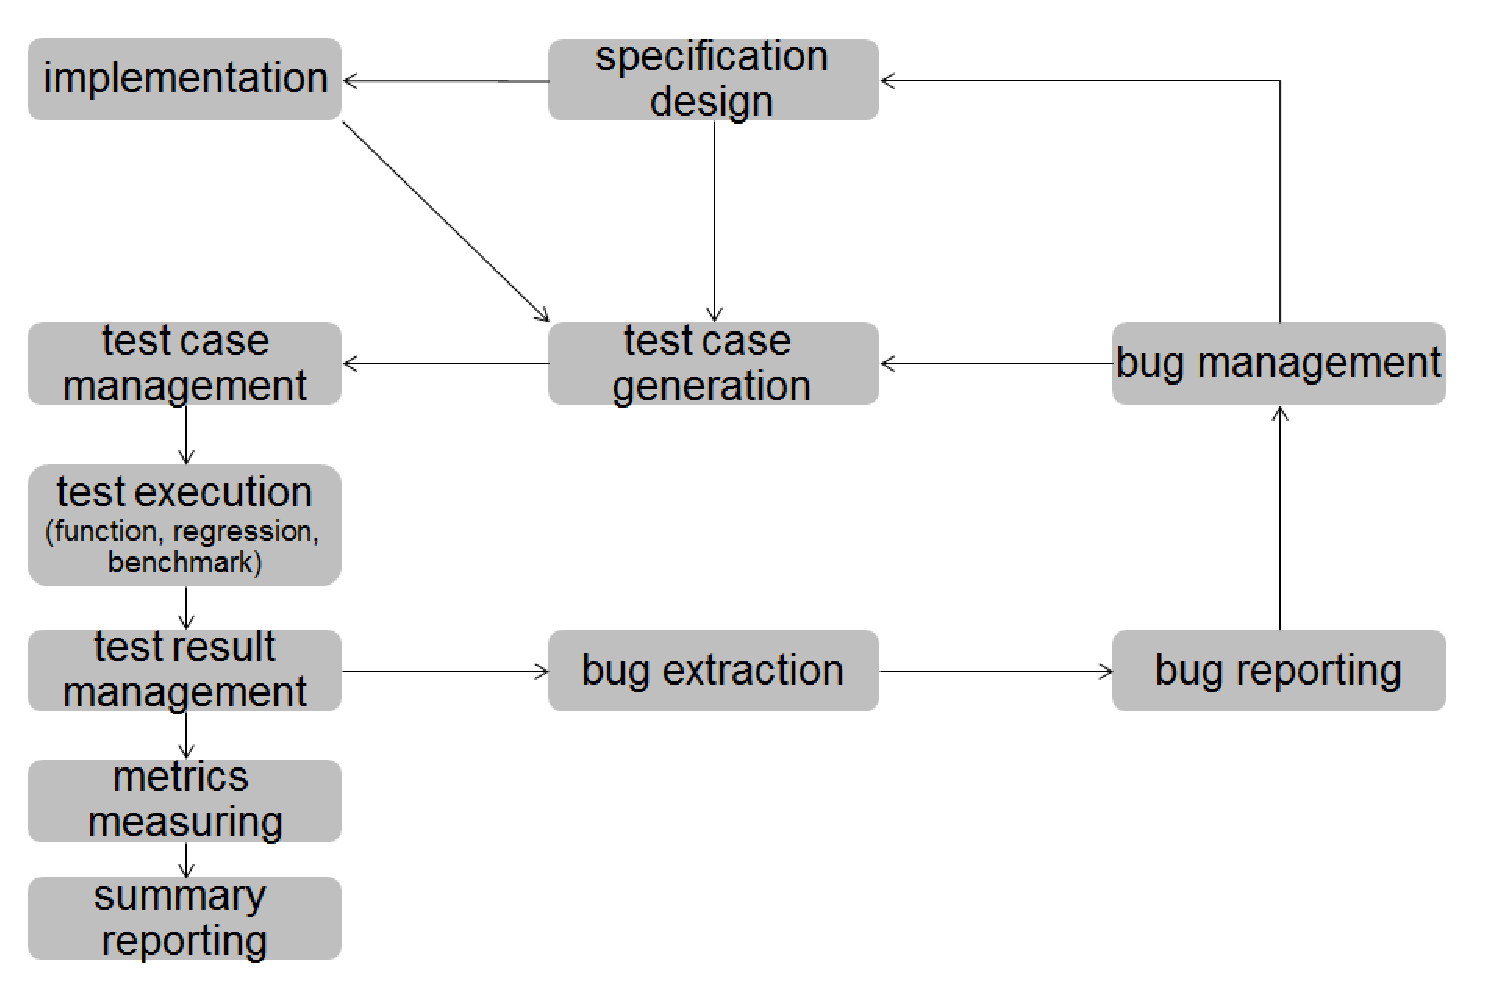
\includegraphics[width=0.8\textwidth]{pic/QA_Tasks.eps}
  \caption{品質管理ライフサイクルを構成する様々なタスク}
  \label{QA_Tasks}
\end{figure}
\par
これらのタスクをサポートするツール類としては、図\ref{QA_Tools}に示すオープンソースの資産が利用可能である。
\begin{figure}[ht]
  \centering
  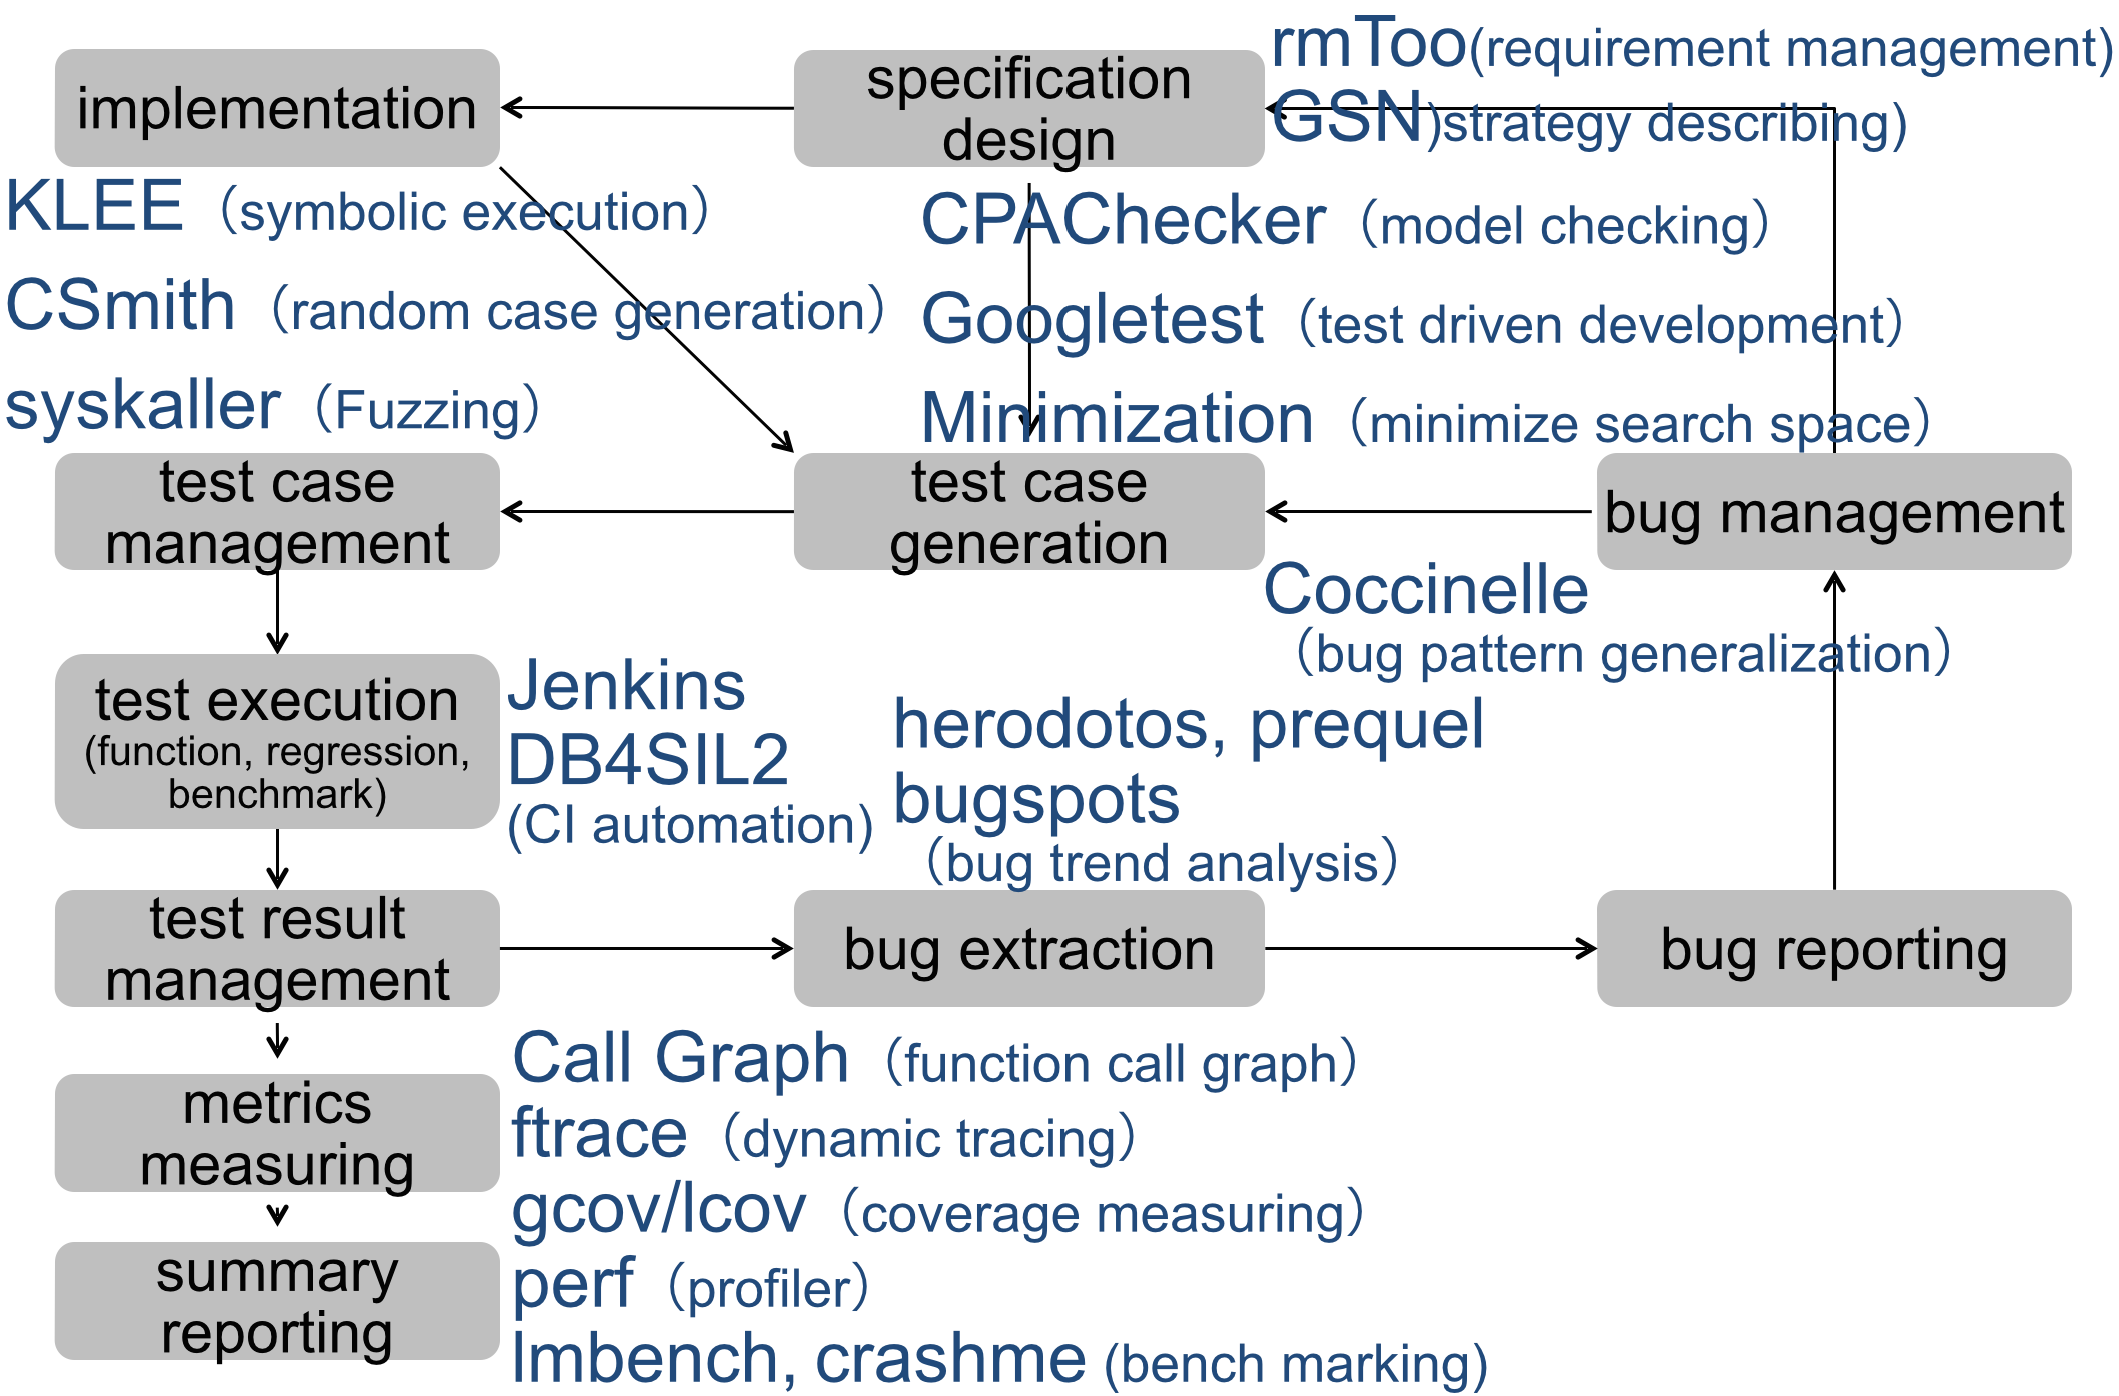
\includegraphics[width=0.8\textwidth]{pic/QA_Tools.eps}
  \caption{品質管理ライフサイクルの各タスクで利用できるツール類の例}
  \label{QA_Tools}
\end{figure}
ただし図\ref{QA_Tools}に示したツール類はあくまでも一例であり、これらのツールを利用すれば各々のタスクを完璧に実施できるという万能なものでもない。
ツールはそれぞれ適用可能なソフトウェアターゲット、得意/不得意な実施内容、実行環境上の制約など様々な性質を持つ。
ツールはあくまでも手段に過ぎず、実際に品質管理ライフサイクルを考える際は「何に対して何を行いたいのか」という目的に対して必要な基準を満たすツール・手法を選定するというアプローチをとることが原則である。
以降は図\ref{QA_Tools}中のツール・手法のうち目的別にいくつかを取り上げそれぞれの調査結果を述べる。

\subsection{バグ検出}
\subsubsection{Coccinelle}
\label{cocci}
\href{http://coccinelle.lip6.fr/}{\acrshort{cocci}} \cite{cocci}はCソースコードのパターンマッチング・変換エンジンである。
例えば、あるAPIを使用している箇所全てについて引数を拡張することや別のAPIに置換するという処理を一括して行うこと、またある論理式・計算式について誤っている表記を一斉に修正すること、さらにC言語の表記を統一するなどコードリファクタリングのような処理を一括して行うことが可能である。
ソースコード中の特定のパターン検索には\acrshort{sm}という非常に柔軟で強力な表現が可能な言語が用いられる。
\acrshort{sm}はスペースや括弧などの表現のばらつきや、変数・関数名の相違などを柔軟に吸収することができ、式の形やデータ構造、処理の流れといったプログラムの意味的な単位に対して作用する。
\acrshort{linux}環境におけるパターンマッチングの技術としては正規表現を使った\verb|sed|コマンドが使われることが多いが、\acrshort{sm}を使った\acrshort{cocci}によるパターンマッチングはそれよりも強力であるという意味で"doped sed"と表現されることがある。
\acrshort{cocci}は"Find once, Fix anywhere"の思想のもとで開発が進められている。
これには、一度\acrshort{sm}でバグパターンを表現してしまえば同種の類似バグを全て改修できる仕組みを作ることで、何度も至る所で同じ修正を繰り返すという無駄な作業を撲滅するという意図が込められている。
\par
\acrshort{cocci} はフランスの研究機関\acrshort{inria}が開発・保守している。
\acrshort{cocci}は関数型言語の\acrshort{ocaml}で書かれており、\acrshort{ocaml}自体も\acrshort{inria}で開発されている。
%\par
\acrshort{cocci}は\acrshort{linux} Kernelのバグ修正に1200件以上の適用実績がある。
\acrshort{cocci}の\acrshort{linux} Kernelにおけるワークフローは、新たに見つかったバグを一般化する形で\acrshort{sm}に書き直して再びソースツリー全体に適用することでその\acrshort{sm}パターンにマッチする同種の残存バグを抽出するというものである。以下に、実際に\acrshort{linux} Kernelに適用実績のある論理演算誤りを修正する\acrshort{sm}の例を示す。
\par
C言語においてnot演算子"\verb|!|"はand演算子"\verb|&|"よりも先に評価されるが、この優先順位関係を誤って認識していたために意図とは異なる論理式を書いてしまう誤りパターンが存在する。
\begin{itembox}[l]{not演算子とand演算子の優先順位を誤った論理演算を含むコード例}
\begin{verbatim}
if(!dma_cntrl & DMA_START_BIT) {
    BCMLOG(BCMLOG_DBG, "Already Stopped\n");
    return BC_STS_SUCCESS;
}
\end{verbatim}
\end{itembox}
\par
この誤りに対して、一般に"\verb|!|式 \verb|&| 定数"のパターンに当てはまるコードを"\verb|!|(式 \verb|&| 定数)"の表記に一括修正する\acrshort{sm}は以下のようになる。
\begin{itembox}[l]{"!式 \& 定数"のパターンを"!(式 \& 定数)"の表記に一括修正する\acrshort{sm}}
\begin{verbatim}
@@
expression E;
constant C;
@@

- !E & C
+ !(E & C)
\end{verbatim}
\end{itembox}
\par
ここで、\verb|@@|で囲まれた箇所はメタ変数宣言部であり、パターンサーチする対象として式(\verb|expression|)、文(\verb|statement|)、型(\verb|type|)、定数(\verb|constant|)、ローカル/グローバル変数(\verb|idexpression|)などを指定することができる。
ここで宣言したメタ変数を使用してパターンの変換ルールを\acrshort{sm}文法に従って表現していく。
この\acrshort{sm}を上記誤りを含むソースファイルに適用すると、\acrshort{cocci}はパターン変換結果を具体的な\verb|diff|形式で出力する。
\begin{itembox}[l]{\acrshort{cocci}によって検出されたパターン変換結果}
\begin{verbatim}
- if(!dma_cntrl & DMA_START_BIT) {
+ if(!(dma_cntrl & DMA_START_BIT)) {
\end{verbatim}
\end{itembox}
\par
\acrshort{cocci}は常にパターンの変換のみを行うものではなく、\acrshort{sm}の書き方によっては\acrshort{cocci}の出力を\verb|diff|形式ではなくパターンマッチしたファイル名と行数のみの表示とするという制御も可能である。
上記のようにして\acrshort{cocci}の出力が得られた後は、それら\acrshort{cocci}の指摘が確かに真のバグであってソースコードに修正を適用するべきものであるかを開発者自身が確認することになる。
ここで\acrshort{sm}の書き方が洗練されていないと、修正する必要のないコードに対しても無駄に\acrshort{cocci}がパターンマッチしてしまい、\acrshort{fp}が大量に出力されてしまうことがある。
\par
これまで実際の\acrshort{linux} Kernel開発でパターン化されバグ修正に貢献実績を持つ\acrshort{sm}が\href{http://coccinellery.org/}{Coccinellery: A gallery of semantic patches} \cite{coccine}で蓄積・公開されている。
Coccinelleryには、式のマクロへの置き換え、API引数追加・削除、API置換、同値表現の統一、デッドロック検出、メモリリーク検出、無効な論理演算検出など\acrshort{linux} Kernel開発で過去にあった既存の修正パターンがほぼ網羅されている。
これらの\acrshort{sm}は再利用することが可能であるが単に使い回せばバグが簡単に検出できるわけではなく、適用する\acrshort{sm}の意図と使い方および期待する出力を各々把握することが必須である。\acrshort{sm}の内容を把握しないまま単に\acrshort{cocci}を実行してもそれらの結果を解釈することができず、また真の指摘が大量の\acrshort{fp}に埋もれてしまうこととなる。
\acrshort{cocci}の\acrshort{fp}に対しては、\href{http://coccinelle.lip6.fr/docs/main_grammar.pdf}{\acrshort{sm}の文法} \cite{sm}に基づいてパターンマッチがより精度よくかつ出力が分かりやすい形となるよう\acrshort{sm}を推敲することが根本的な対策となる。
Coccinelleryに蓄積されている\acrshort{sm}は既に\acrshort{linux} Kernelに適用済みのものであるので、それらを全て再度適用することにはあまり意味がない。
蓄積された\acrshort{sm}の一つの使い方としては、ソースコードに変更を加える前後で\acrshort{cocci}を実行して得られた指摘を\acrshort{fp}含めて比較し、変更前に無く変更後にのみ存在する差分指摘を得ることで回帰テストを効率化する戦略が考えられる。
\par
\acrshort{cocci}は汎用的なセマンティックパターンサーチエンジンであるため、ソースコードのバグ検出以外にも広く様々な使い道が考えられる。
例えばセキュリティ対策としてのコード難読化(code obfuscation)のために、以下のように意味的に等価なコード変換が\acrshort{cocci}で実現できる可能性がある。
\begin{itemize}
  \item 関数名、変数名のランダム文字列への変換
  \item 数値演算、論理演算の等価で複雑な形への変換
  \item 制御構造の複雑化(例:ループ制御の再帰呼び出しへの等価変換)
  \item 関数呼び出し関係の値渡しから参照渡しへ等価変換
  \item データ構造の複雑化(例:構造体の分解または統合)
\end{itemize}
\par
また、\acrshort{cocci}の派生ツールとして、\href{https://github.com/regit/coccigrep}{Coccigrep} \cite{coccigre}というツールがある。
Coccigrepは\acrshort{sm}の文法に基づいてCソースコード中でセマンティック検索するツールで、次のような解析手段を提供する。
\begin{itemize}
  \item 特定の型または特定の構造体の変数がどこで使われているか調べる
  \item 特定の構造体のフィールドがどこで参照されているか調べる
\end{itemize}
\newpage
\subsubsection{Csmith}
\label{compveri}
\href{https://embed.cs.utah.edu/csmith/}{\acrshort{csmith}} \cite{csmith}はCプログラムのランダムジェネレータであり、コンパイラの動作検証を行う目的で使用される。
\acrshort{csmith}は\acrshort{gcc}、\acrshort{llvm}、および商用コンパイラの自動検証とバグ検出に長い実績がある。
特に、コンパイル最適化オプション有効時の誤り検出に顕著な貢献をしてきた。
\par
機能安全対応のソフトウェア開発においては、開発ツール自体についても厳格に採用基準を定め評価を行うことが求められる。
\acrshort{iec61508}-4 3.2.11 において開発ツールは認証対象となるソフトウェアへの影響度に応じてT1, T2, T3の3段階のクラス分けがなされており、そのうちコンパイラはソフトウェア(バイナリ)生成に直接関与するツールとしてT3クラスに分類される。
コンパイラの誤動作は直ちにソフトウェア誤動作の要因となるため、コンパイラの正当性評価には膨大な量のテスト結果と使用実績がエビデンスとして求められる。
実績として十分なエビデンスを得るためには認証対象となるコンパイラについて固定されたバージョンとコンパイルオプションの下、様々な用途の数多くのアプリケーション適用例が必要である(\acrshort{iec61508}-3 7.4.4.2 )。
そのためアプリケーション開発元が単独でコンパイラ認証を行うことは事実上困難であり、機能安全対応のソフトウェア開発には第三者機関によって認証取得済のコンパイラを利用するかまたは専門のコンパイラ評価サービスを利用することが一般的であった。
しかし\acrshort{sil2linuxmp}が対象とするソフトウェアはオープンソースであり、開発ツールも全てオープンソースでなければないという制約があるため、次の2つの理由からコンパイラ検証を第三者に依存することができない。
\begin{itemize}
  \item 認証対象プラットフォームを構成する\acrshort{oss}ソフトウェアのアップデートに依存してコンパイラも持続的なアップデートを前提とするためバージョンを固定できない
  \item コンパイラの検証手法自体もオープンな技術である必要があり、特定の第三者の技術にvendor lock-inされる状態は許容されない
\end{itemize}
\par
以上の制約から、機能安全対応の\acrshort{oss}・\acrshort{linux}プラットフォーム開発で使うコンパイラ検証プロセスは、オープンな技術であり、アップデートにも耐えられるよう検証プロセスが自動化可能で、過去の検証資産を再利用して反復適用できるような性質を持つものである必要がある。
\acrshort{csmith}で生成したエビデンス自体ではコンパイラの正当性を証明するのに十分ではないものの、\acrshort{csmith}は\acrshort{sil2linuxmp}プロジェクトで求められる必要な性質をもつコンパイラ検証ツールとして有効である。
\par
\acrshort{csmith}は次のようなワークフローでコンパイラの正当性検証を行う。
ここでは例として\verb|gcc-4.9|を最適化オプション\verb|-O2|で使用するときの検証方法を挙げる。
\begin{enumerate}
  \item \verb|csmith|コマンドでCプログラムをランダム生成する。
  \begin{itemize}
    \item[] \verb|$ csmith -s <seed> random.c|
  \end{itemize}
  \item 生成したプログラムを検証対象を含む複数のコンパイラにかける
  \begin{itemize}
    \item[] \verb|$ gcc-4.8 -O0 random.c -o random_4.8_O0|
    \item[] \verb|$ gcc-4.9 -O0 random.c -o random_4.9_O0|
    \item[] \verb|$ gcc-4.9 -O2 random.c -o random_4.9_O2|
  \end{itemize}
  \item 生成した複数のバイナリを各々実行し出力結果を比較する
  \begin{itemize}
    \item[] \verb|$ ./random_4.8_O0|\\\verb|checksum = 54A570D1| $\cdots$\verb|gcc-4.8|の\verb|-O0|でコンパイルしたバイナリの実行結果
    \item[] \verb|$ ./random_4.9_O0|\\\verb|checksum = 54A570D1| $\cdots$\verb|gcc-4.9|の\verb|-O0|でコンパイルしたバイナリの実行結果
    \item[] \verb|$ ./random_4.9_O2|\\\verb|checksum = 54A570D1| $\cdots$\verb|gcc-4.9|の\verb|-O2|でコンパイルしたバイナリの実行結果
  \end{itemize}
\end{enumerate}
\par
全ての実行結果の出力(\verb|checksum|値)が一致すれば、ここでランダムに生成したプログラム\verb|random.c|に関する検証は成功である。
もしいずれかの結果が他と異なる出力となる、またはバイナリ実行が失敗する、またはコンパイル自体が失敗する場合は、その事象を該当コンパイラおよびオプションの組合せに関するバグとして調査する。
以上の手続きを、\verb|csmith|で生成するランダムCプログラムの種を変えながら繰り返し実施し続ける。
検証成功したランダムプログラム数が増えるほど、その実績がそのコンパイラとオプションの組み合わせに対する品質を保証するエビデンスとなる。
\par
\acrshort{csmith}が生成するランダムプログラムがコンパイラの正当性を示すために十分に有効なテストケースとなるためには、そのプログラムがC言語で表現可能な出来る限り多様なコードを含んでいなければならない。
しかしこの要件は、コンパイラのテストケースとして使われるプログラム
%\acrshort{csmith}でランダム生成したプログラム(コンパイラテストケース)
はC言語仕様で不定または未定義の振る舞いをするコードを含んでいてはいけないという制約とトレードオフの関係にある。
例えば、\verb|a = f(b) + g(b)|という式について\verb|f(b)|と\verb|g(b)|のどちらが先に評価されるかは不定である。\verb|f(b)|と\verb|g(b)|が共に\verb|b|を変更するとき、コンパイラの実装によっては\verb|f(b)|と\verb|g(b)|の評価順序が逆転してその結果式全体の評価結果\verb|a|が異なる可能性があるが、この挙動はC言語仕様では不定であるのでどちらの挙動も正しい。
また、ゼロ除算、$-1$での剰余、配列領域外アクセス、NULLポインタ開放、整数オーバーフロー、未初期化変数の参照などC言語仕様上未定義の動作となるコードは、コンパイラによっては気を利かせた挙動をするものがあるものの、ほとんどの場合はプログラムがクラッシュする結果となるため有効なテストケースとならない。
このように、コンパイラの正当性検証テストケースとしてはC言語仕様で厳密に定義された振る舞いをするコードのみからなるプログラムを使用しないと、上記の\acrshort{csmith}のワークフローでは\acrshort{fp}が大量に生成されてしまう。
\par
このため、\acrshort{csmith}のアルゴリズム開発では当初から現在まで「不定または未定義挙動のコードを含まずコンパイルエラーにならにコードで可能な表現を多く含むランダムプログラム生成」をいかに正確に実現するかに努力が払われてきた。
生成される\acrshort{fp}には不定/未定義挙動が原因であるものと既知問題であるものがあり、真のバグ選別および有効なバグレポートの作成がとても困難であるという経験から、\acrshort{csmith}を使ったコンパイラ検証プロセスの自動化とバグトリアージ(\acrshort{fp}の山から真の指摘を抽出する)方法の開発が課題であるとされている。
これまで\acrshort{csmith}が適用された実績がある\acrshort{gcc}はごく一部のバージョンとオプションの組合せに対してのみであり、\acrshort{gcc}のアップデートに対して最新のバージョンと最適化オプションの組合せ検証網羅および\acrshort{csmith}による検証作業が追いついていない状況である。
また\acrshort{csmith}による検証自体をどこまでやれば十分であるかを一様に判断することが困難である。機能安全対応の際は、例えば蓄積されたテスト結果を用いて「統計的に残存バグがあと何件以下」というような論理的な根拠を構築して認証機関に十分性を示すことが求められる。
\subsection{テストケース生成}
\subsubsection{KLEE}
\label{klee}
\href{https://klee.github.io/}{\acrshort{klee}} \cite{klee}は\acrshort{se}ツールの一種で、既存のソースコードを元に同値分割テストケースを自動生成する目的で使用できる。
\acrshort{klee}は与えられたCソースコードから可能な実行パスに遷移するための引数や変数の状態組合せを探索して模擬実行する(\acrshort{se})。
以下に\acrshort{klee}がCソースコードを元にテストケースを生成する挙動の例を示す。
\begin{itembox}[l]{テスト対象関数の例}
\begin{verbatim}
int get_sign(int x) {
  if(x == 0)
    return 0;

  if(x < 0)
    return -1;
  else
    return 1;
}
\end{verbatim}
\end{itembox}
\par
上記関数に対して\acrshort{klee}は以下のように振る舞う。
\begin{enumerate}
  \item 関数中の全分岐(\verb|if-else|)を特定する
  \item 特定した各分岐に遷移するための変数\verb|x|の条件を探索する
  \item 探索した各条件について具体的な代表値を一組決める
\end{enumerate}
\par
この結果3パターンの\verb|x |$ = \{0, 16843009 (> 0), -2147483648 (< 0)\}$で\verb|get_sign()|を呼ぶテストケースが生成される。
生成された3つのテストケースはそのまま何度でも再利用できるため例えば回帰テストへの応用が考えられる。
\par
\acrshort{iec61508}は同値分割テストケース生成について仕様に基づく方法とプログラムの内部構造に基づく方法の2通りを示唆しており(\acrshort{iec61508}-7 Ed2 C.5.7)、このうち\acrshort{klee}はプログラムの内部構造からテストケースを生成するツールとして適用できる。
\acrshort{klee}ではソースコードがあればテスト対象の仕様を特に知らなくてもテストケース生成が可能であるが、関数引数をシンボリック変数にしてテスト対象を呼び出すためのテストドライバの作成は必要となる。
\par
\acrshort{klee}のアルゴリズムはヒューリスティック探索に基づくため100\%分岐網羅を保証するものではない。
上記の例のように単純なプログラムであれば100\%分岐網羅を達成することができるが、実用上の大きなプログラムでは計算コスト上の制約が問題となる。
\acrshort{klee}のパフォーマンスを向上させるためには、例えば無駄な探索をさせないようにシンボリック変数の動く範囲を指定することが有効である。
テスト対象となる関数の引数が数値ならばその上限と下限を、文字列ならば各文字が取り得る値を、または論理式を使い複数の引数の制約関係を表現することもできる。
これを利用すれば、シンボリック変数の条件をテストドライバ側で指定することで入力仕様に基づいたテストケースを設計することができる。
また、用意された4種類の探索アルゴリズムから適当なものを選択したり、アルゴリズムをラウンドロビンで組合せたり、最大探索深さやタイムアウト時間の設定ができたり、優先して探索するシンボリック変数の条件が指定できるなど探索戦略を柔軟に調整する手段が提供されている。
\par
\acrshort{klee}は\acrshort{llvm}プラットフォーム上で動作するため、\acrshort{llvm} bitcodeにコンパイルできないプログラムには\acrshort{klee}が適用できないという制約が存在する。
\acrshort{sil2linuxmp}では\acrshort{bb}に対して\acrshort{klee}を使用してテストケース生成と同値分割テストを実施することが検討されている。
\acrshort{klee}はその性質上、プログラムの挙動が入力のみに依存して決定的であるものに対して有効で、外部からの割り込み、並列実行、タイミング等が挙動に影響する対象は適用が困難である。そのため\acrshort{linux} Kernelに対しては\acrshort{klee}による解析は適さない。
%\subsubsection{Syskaller}
\subsection{反例検出}
\subsubsection{CPAChecker}
\href{http://cpachecker.sosy-lab.org/}{\acrshort{cpa}} \cite{cpa}はCプログラムの各コードブロックへの到達可能性を検証するモデルチェックツールである。
Cソースコードを入力として制御フローオートマトンを導出し、予め定義されたエラー状態へ遷移する可能性を解析する(図\ref{cpa})。
CPAは"Configurable Program Analysis"の頭文字であり、数あるプログラム状態遷移解析ツールの中でも、設定次第で一つのツールで複数用途の解析に使用可能であることが特徴である。
例えば、メモリアクセス違反など特定の動的挙動に絞って解析を行う場合や、仕様検証のために正確性を重視したモデルチェックを行う場合などで、計算資源と正確性のトレードオフを考慮してメモリ割り当て量やタイムアウト時間などを制御することや、検証項目によってアルゴリズムを選択することができる。
これらの検証アルゴリズム・パラメータセットは予め用意された設定が180存在しており、目的に従って既存の設定を選択使用することができる。
\acrshort{cpa}はLinux Driver Verification Project (linuxtesting.org)で採用されており、Linuxデバイスドライバに対して150件以上のバグ修正実績がある。
\begin{figure}[ht]
  \centering
  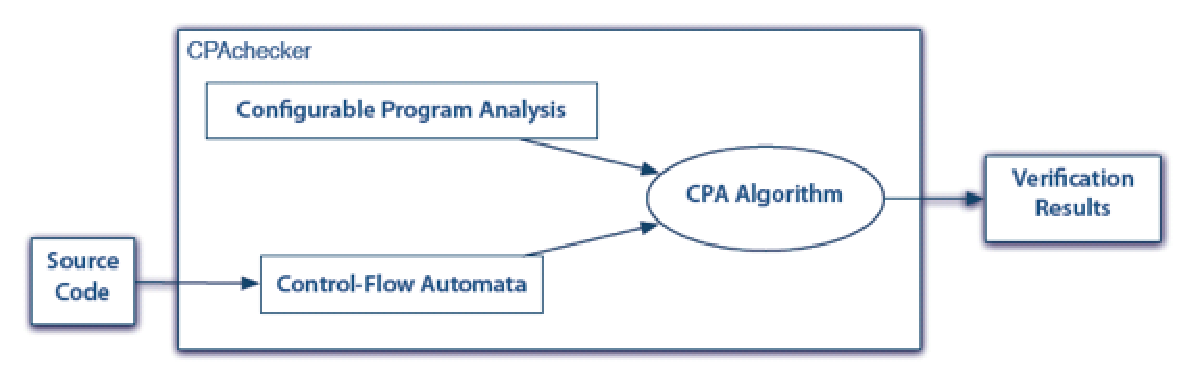
\includegraphics[width=\textwidth]{pic/cpa.eps}
  \caption{\acrshort{cpa}のワークフロー}
  \label{cpa}
\end{figure}
\par
以下に、プログラムのエラー状態への遷移可能性を\acrshort{cpa}によって解析する例を示す。
\begin{itembox}[l]{定義されたエラー状態に到達し得るミスがあるコード例}
\begin{verbatim}
#include <stdio.h>

int main(void) {

  double x, y;

  // xで受け取った実数の絶対値をyに入れる
  scanf(“%lf”, &x);
  // 負数かどうかの判定を誤って-1以下の条件としてしまった実装
  y = (x <= -1) ? (-1) * x : x;

  printf(“abs(%lf) = %lf\n”, x, y);

  // 計算した絶対値が非負でなかったらエラーとする
  if(y < 0) {
    goto ERROR;
  }

  return 0;

// CPACheckerはソース中の”ERROR”ラベルかasseart()を見つけて
// そこへ遷移する条件(反例)を探す。このケースでは”ERROR”ラベルの代わりに
// asseart(y < 0); としても同じ検証ができる。
ERROR:
  return 1;
}
\end{verbatim}
\end{itembox}
\par
\acrshort{cpa}はこのプログラムファイルと検証アルゴリズムの設定およびパラメータセットを読み込んで、検出されたエラー状態に遷移するための変数の状態を探索する。
出力はには、\acrshort{gv}フォーマット(.dot)による\acrshort{cfa}と\acrshort{art}が含まれる。
\acrshort{cpa}の結果はReport Generatorによりwebブラウザで視覚的に表示できる形式で出力することが可能である(図\ref{cpareport})。
\begin{figure}[ht]
  \centering
  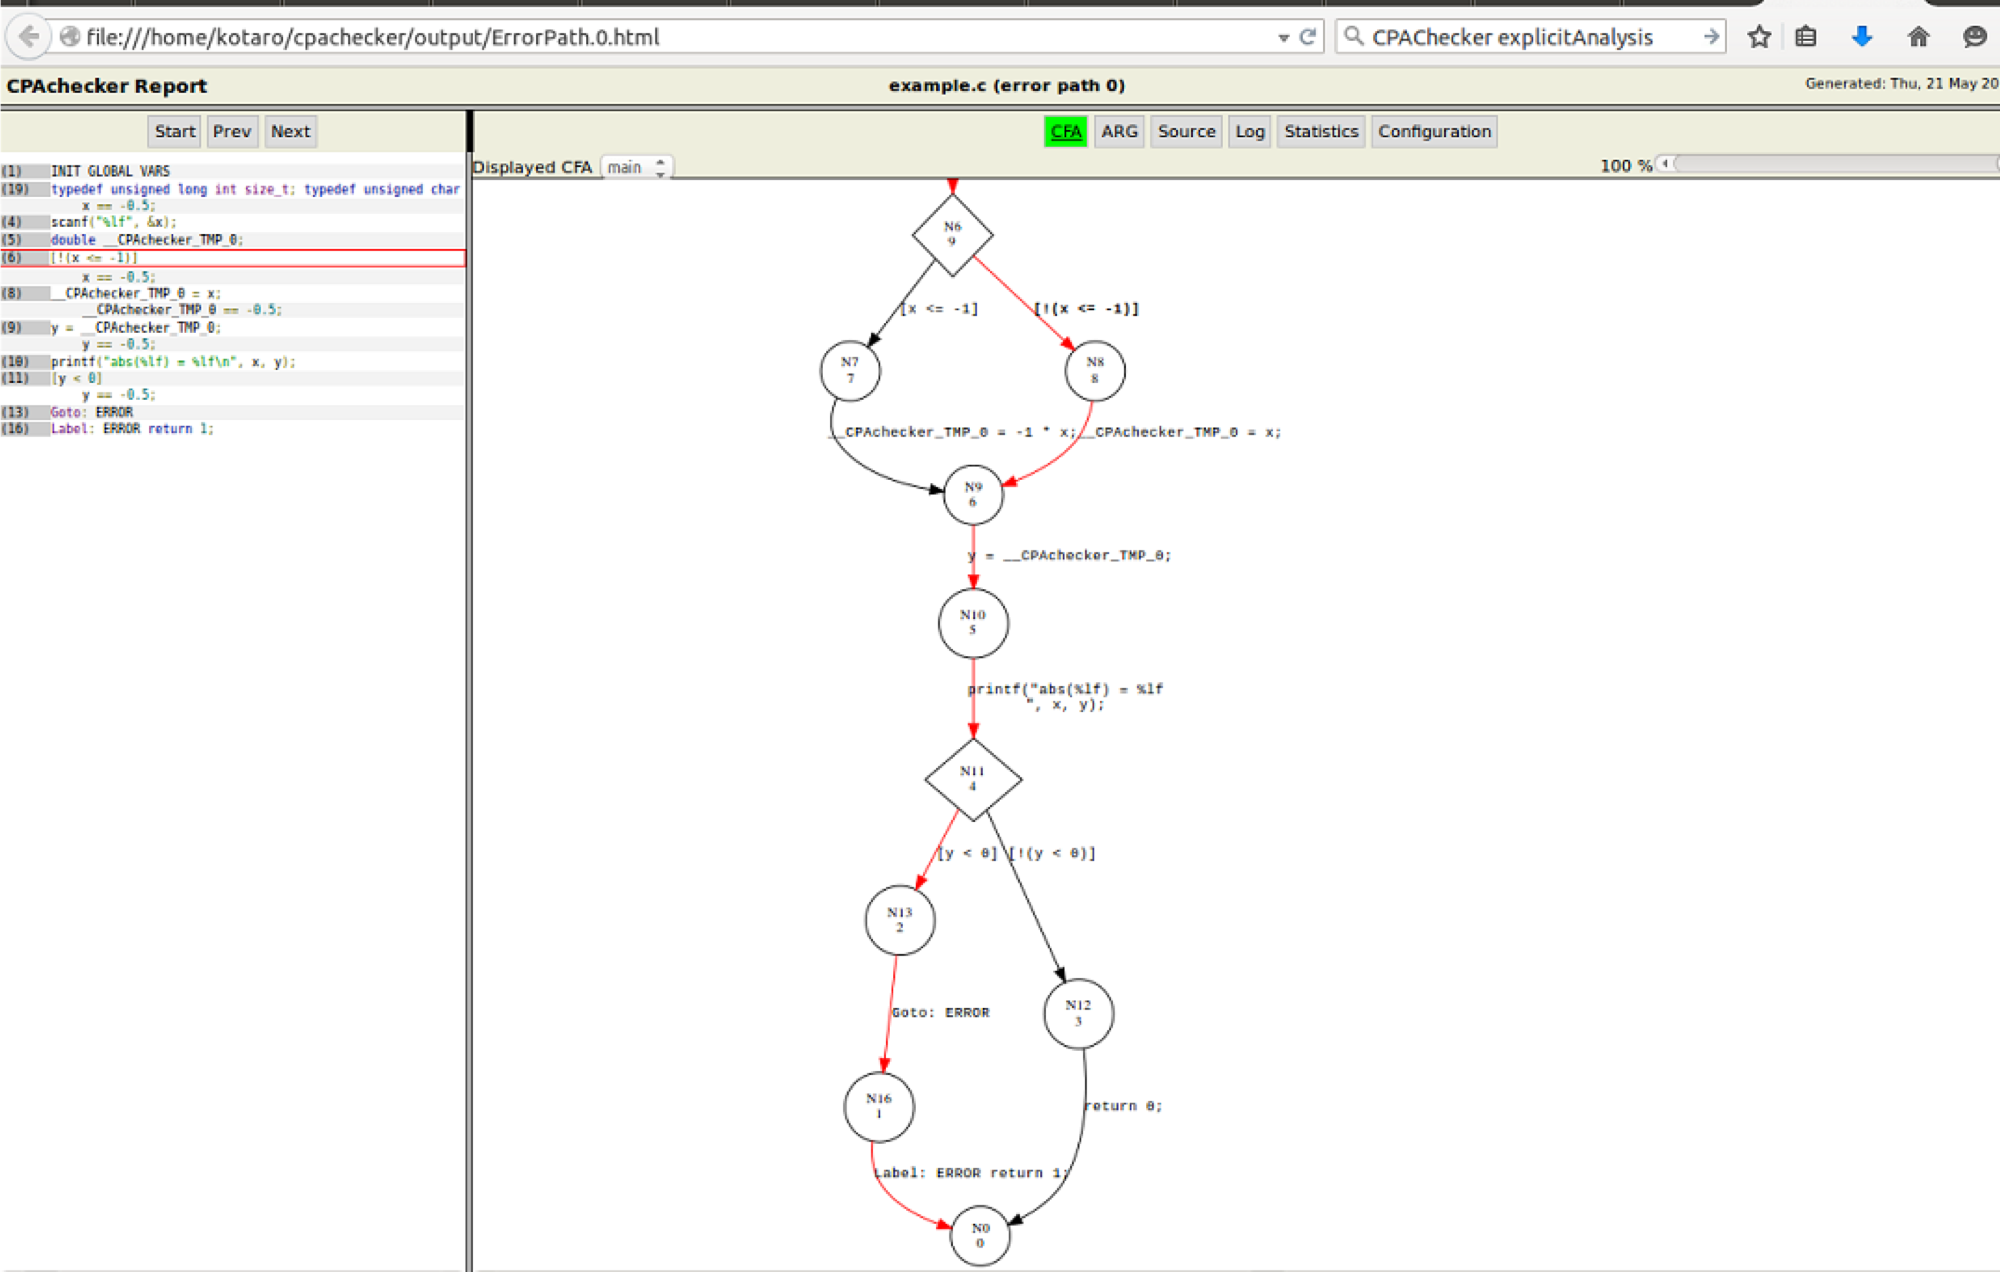
\includegraphics[width=\textwidth]{pic/cpareport.eps}
  \caption{\acrshort{cpa} Report Generatorの出力例}
  \label{cpareport}
\end{figure}
\par
図\ref{cpareport}のReport Genetatorの出力右半分には関数毎の状態遷移図を表す\acrshort{cfa}が表示されており、各エッジやノードをクリックすると該当する制御文や宣言などのコードにジャンプすることができる。
ここで、検出されたエラーパスは赤く表示されており、このパスを通る際のコールスタックがレポートの左半分に表示されている。
コールスタックの各行からも、該当する\acrshort{cfa}のエッジまたはノードにジャンプすることができる。
図\ref{cpareport}の左画面(6)の次の行に表示されている\verb|x == -0.5|が、探索された反例(Counter Example)の具体値であり、これによってこのプログラムは\verb|x == -0.5|のときに\verb|ERROR:|ブロックに遷移しプログラムが異常停止することが分かる。
\par
以上の使用例に代表されるように、\acrshort{cpa}は予め定義されたエラー状態に到達し得るかどうかの判定(Reachability Analysis)と、エラー状態に遷移し得る場合はその条件(Counter Example)を具体的な変数状態で探索する。
また検証アルゴリズムの設定によっては、NULLポインタアクセスやバッファオーバーフローなどのメモリアクセス違反が発生し得るかどうかの判定も可能である。
予めエラー状態がコード中に定義されていればそこに遷移する条件を自動的に検出できることから、\acrshort{gt}等のテスト駆動開発手法と上手に併用出来れば強力な回帰テストフレームワークを構築できる可能性がある。
\par
\acrshort{cpa}が適用可能なC言語表現は、ループ、配列、条件分岐、ポインタ、ヒープ、再帰、浮動小数点表示等と幅広く、\acrshort{cpa}は特に制御フローとメモリアクセスの安全性解析を得意とする。
一方で、深くネストされたループやメモリを大量に消費する再帰構造を持つフローの解析は得意でなく、\acrshort{cpa}は無限ループの検出やデッドロックの検出を行うことができない。
また、マルチスレッド等の並列実行構造を持つフローの解析にも対応していない。
図\ref{svcomp}は、2015年に行われた国際的なソフトウェア検証コンペティション\href{http://sv-comp.sosy-lab.org/2015/results/index.php}{\gls{sv}の総合結果} \cite{sv}である。
\acrshort{sv}では様々な種類の検証課題に対して各々検証プラグラムのベンチマークが測定される。
\begin{figure}[ht]
  \centering
  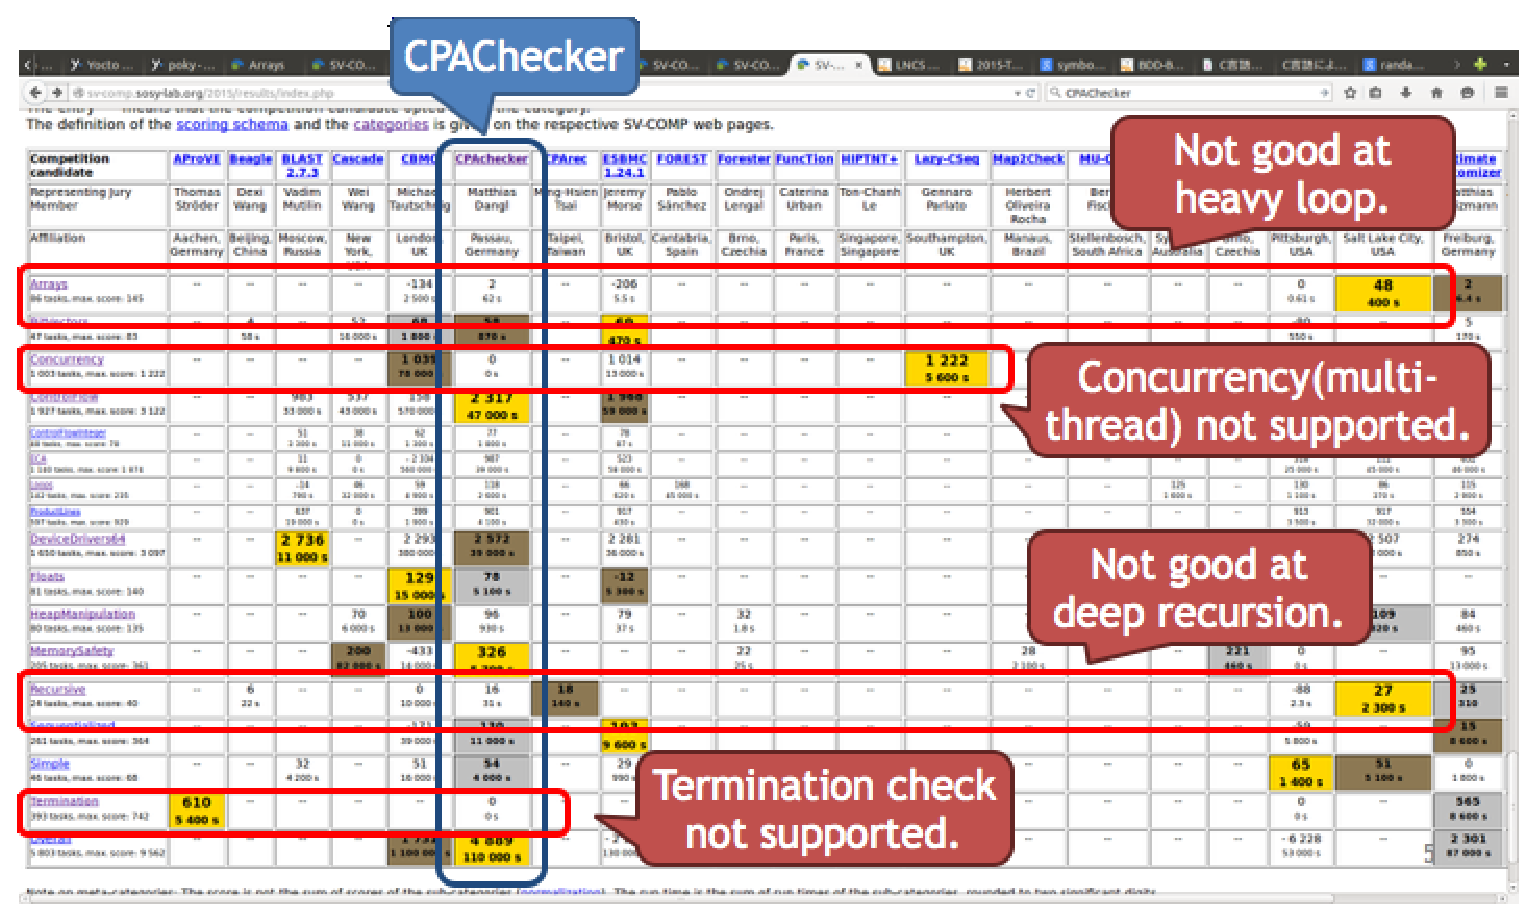
\includegraphics[width=\textwidth]{pic/svcomp.eps}
  \caption{\gls{sv}2015 の総合結果}
  \label{svcomp}
\end{figure}
\par
\acrshort{cpa}は制御フローやメモリアクセスの安全性解析および\acrshort{linux}デバイスドライバの解析で圧倒的なパフォーマンスを示しており総合評価でもトップの成績を残している。
ただし、先述したように深いループ・再帰の解析は不得意で停止性検証および並列実行の解析は対応していないため、これらの検証課題に対しては他のツールが優位となっている。
例えばプログラムの停止性検証(termination check)では\href{http://aprove.informatik.rwth-aachen.de}{\gls{aprove}} \cite{aprove}という停止性検証に特化した強力なツールが存在し、実際のデバイスドライバの検証にも大きな貢献をしてきている。
停止性検証は古くから研究されている問題で、制御フローの解析問題とは独立にその分野自体に長い蓄積がある。
全ての問題に対応する万能なツールを追求することは本質的ではなく、あくまでも目的とする検証対象に合致したツール・手法を選択しそれらの制約をよく把握した上で適切なツール・手法を使用することが重要である。
\subsection{メトリクス測定}
\subsubsection{CodeViz}
\label{cv}
\href{http://www.csn.ul.ie/~mel/projects/codeviz/}{\acrshort{cv}} \cite{cv}はC/C++プログラムの関数呼び出し関係を視覚化する関数コールグラフ生成ツールである。
\acrshort{sil2linuxmp}では動的トレーシングツールの結果と組み合わせて呼び出し関係のカバレッジを測定する用途で使用することが検討されている(詳細は\ref{callgraph}項で記載)。
関数コールグラフ生成ツールは、ソースコードを静的に解析してグラフを得るものと、実際にプログラムを動かしたときの挙動から動的にグラフを得るものとに大別できる。
このうち\acrshort{cv}は静的に関数コールグラフを生成するツールである。
静的コールグラフ生成ツールとしては他に\acrshort{gnu}プロジェクトの\acrshort{cflow}がある。
\acrshort{cflow}と比較して、\acrshort{cv}は関数ポインタを介した関数呼び出し関係も出力に反映できるという利点がある。
図\ref{vfs}は、\acrshort{linux} Kernel 4.3.3ツリーの\verb|fs/read_write.c|に対して\verb|vfs_read()|関数から先のコールグラフを生成した例である。
\begin{figure}[ht]
  \centering
  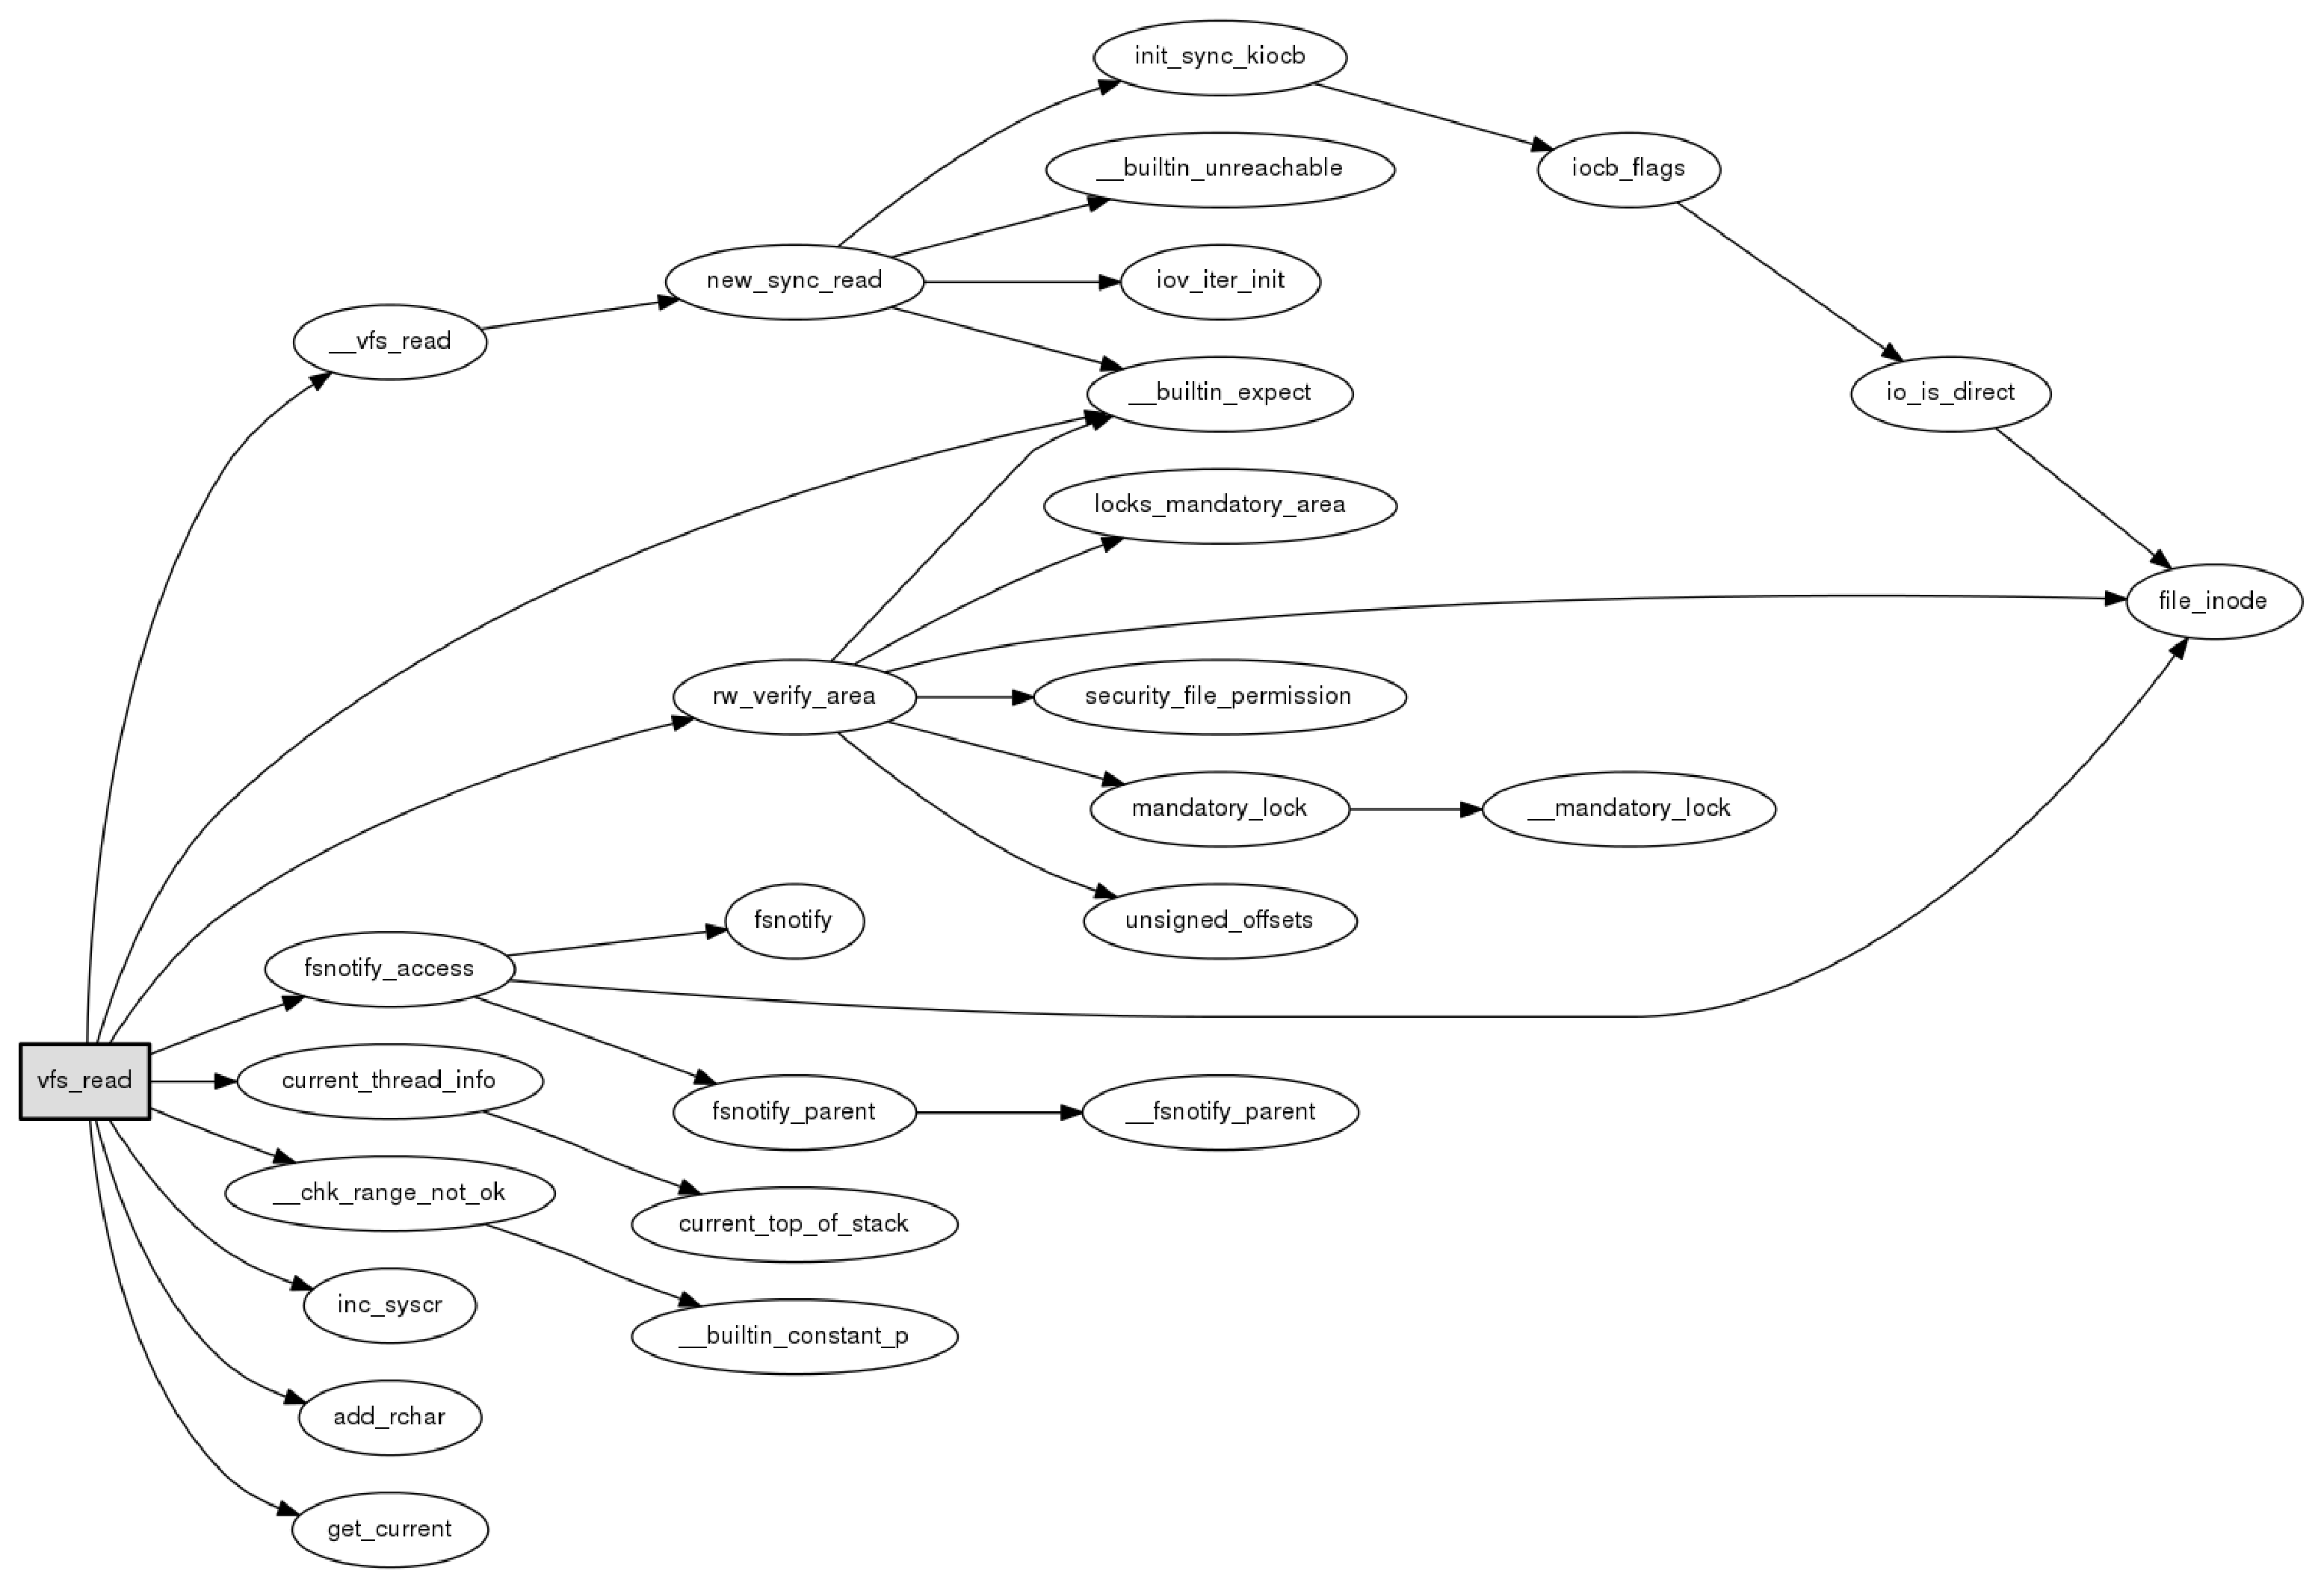
\includegraphics[width=0.8\textwidth]{pic/vfs_read.eps}
  \caption{\acrshort{linux} Kernel fs/read\_write.cのvfs\_read()関数コールグラフを\acrshort{cv}で生成した例}
  \label{vfs}
\end{figure}
\par
\acrshort{cflow}と比較して、\acrshort{cv}の出力は次の点でより洗練されたものとなっている。
\begin{itemize}
  \label{cv_vs_cflow}
  \item \verb|vfs_read()|と\verb|__vfs_read()|を区別する(\acrshort{cflow}は\verb|__|接頭辞が無視され両者が同一ノードになってしまう)。
  \item 意図しないマクロ\verb|likely()|や\verb|unlikely()|のコールグラフへの出現が抑制されている(\acrshort{cflow}では関数ノードとして出現してしまう)。
  \item \verb|loff_t|など独自定義の型名が正しく処理されている(\acrshort{cflow}では誤って\verb|loff_t|が関数ノードとして出現してしまう)。
\end{itemize}
\par
\acrshort{cv}は、コールグラフデータの生成手段としてdepnとnccという二つの方法を提供している。
depnは特定の\acrshort{gcc}のバージョン(3.4.6か4.6.2)に対して専用のパッチを当てたものを使用してコールグラフデータを生成するため手順がやや複雑である。
\href{http://students.ceid.upatras.gr/~sxanth/ncc/}{ncc} \cite{ncc}は特に\acrshort{gcc}に対するパッチは必要なく手順が簡単である上、関数ポインタを介した呼び出し関係も表現することができる利点がある。
\acrshort{sil2linuxmp}では、手順の簡易さと関数ポインタを扱えるという利点からnccを利用する検討が進んでいる。
nccはソースコードのブラウジング用途に開発されたコンパイラである。
なお、グラフデータの視覚化は\acrshort{cv}付属のツールを用いて画像を生成する方法と、nccパッケージに付属する\acrshort{gv}データ(.dot)変換ツールを用いる方法がある。
関数コールグラフを利用した呼び出し関係のカバレッジメトリクス測定として\acrshort{sil2linuxmp}で検討されている方法については\ref{callgraph}項で記載する。
%\subsubsection{ftrace}
\newpage
\subsubsection{syzkaller}
\href{https://github.com/google/syzkaller}{\acrshort{syzkaller}} \cite{syzkaller}は、\acrshort{linux} Kernelシステムコールに対する\acrshort{fuzzer}プログラムである。
Fuzzerとは、大量のランダムデータ・ランダムテストケースを生成・実行することで検査対象プログラムのミスや脆弱性を見つけるテストプログラムの総称を言う。
\ref{klee}項で触れた\acrshort{csmith}はコンパイラに対する\acrshort{fuzzer}である。
\acrshort{syzkaller}はシステムコールに対するカバレッジを指標にテストケースを自動生成・実行する。
これを利用すると、ターゲットシステムの\verb|debugfs|からシステムコールに対するテストカバレッジ情報を取得できたり、クラッシュ情報やテスト結果を取り出して開発ホスト側のwebインタフェースでサマリを表示したりということが可能になる(図\ref{syzkaller})。
\begin{figure}[ht]
  \centering
  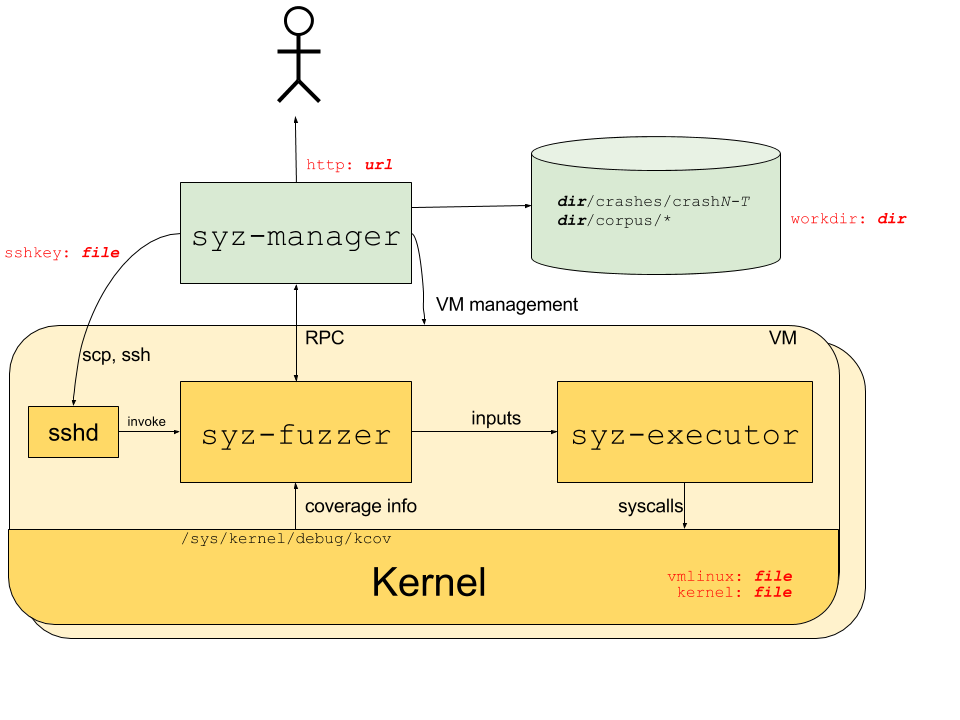
\includegraphics[width=0.8\textwidth]{pic/syzkaller.eps}
  \caption{\acrshort{syzkaller}システムの全体アーキテクチャ}
  \label{syzkaller}
\end{figure}
\par
\acrshort{syzkaller}は2015年10月に開発が始まった新しいプロジェクトであるため成熟度は十分でなく、現在サポートされるプラットフォームは\acrshort{qemu}のみで他の仮想マシンや物理ターゲットボードは未サポートである。
また現状は導入の前提条件として最新の\acrshort{gcc}を自前でビルドする必要があったり、\acrshort{linux} Kernelに特別にパッチを当てる必要があったりと手順に難がある。
\acrshort{sil2linuxmp}では\acrshort{linux} Kernelシステムコールのテストカバレッジ向上とメトリクス測定のために\acrshort{syzkaller}利用すること想定して調査が継続されている。
\subsection{バグ選別}
\ref{cocci}項で述べた通り、\acrshort{cocci}はそれ単独で用いると大量の\acrshort{fp}を生成してしまうため、真のバグをいかに選別するかが効率的なバグ検出にとって重要となる。
\subsubsection{Herodotos}
\href{http://coccinelle.lip6.fr/herodotos/docs/herodotos.html}{\acrshort{hero}} \cite{hero}は、\acrshort{cocci}の\acrshort{fp}を抑制する目的で\acrshort{cocci}と同じ\acrshort{inria}が開発しているツールで、特定のバグパターンの出現傾向を世代間にわたって解析することができる。
\acrshort{sm}で一般化したバグパターン各々についてバグのトレンドと残存期間などを視覚化することで、そのプロジェクトの開発プロセスの安定性や健全性を示す根拠の一つとして利用することが\acrshort{sil2linuxmp}では検討されている。
図\ref{herograph}は、"badzero"というバグパターンが\acrshort{linux}、Wine、VLC、OpenSSLの各プロジェクトについて世代ごとにどの程度残存していたかをグラフで示したものである。
\begin{figure}[ht]
  \centering
  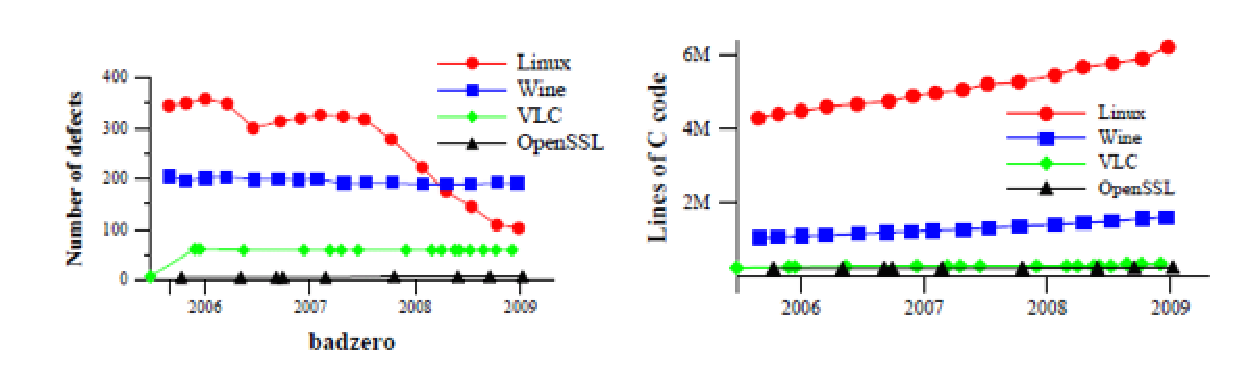
\includegraphics[width=\textwidth]{pic/herograph.eps}
  \caption{各プロジェクトの各世代に対する"badzero"バグの存在数(左図)と各プロジェクトの各世代でのコードサイズ(右図) https://hal.inria.fr/inria-00406306/PDF/RR-6984.pdfから引用}
  \label{herograph}
\end{figure}
\par
図\ref{herograph}から、\acrshort{linux} Kernelはその成長に伴ってbadzeroバグが積極的に改修されているのに対して、その他のプロジェクトでは同種のバグがほぼ放置されたままとなっていることが分かる。
\par
図\ref{heroview}に\acrshort{hero}ワークフローの概要を示す。
\acrshort{hero}は、解析対象となる特定パターンの出現場所が記録された\textcircled{\scriptsize 2}"pattern occurrance reports"と、解析対象となるソフトウェアバージョン間の差分情報\textcircled{\scriptsize 3}"code changes"を入力とする。
ここで、\textcircled{\scriptsize 2}"pattern occurrance reports"は\acrshort{cocci}の出力で、\textcircled{\scriptsize 3}"code changes"は\acrshort{gnu} diffの出力である。
図\ref{heroview}中の"code pattern"は\acrshort{sm}、"pattern matching tool"は\acrshort{cocci}、"diff tool"は\acrshort{gnu} diffを意味する。
"tracking environment"に相当する箇所は、解析対象となるバグパターンを記載した\acrshort{sm}と解析対象の各バージョンのソフトウェアを含めて自前で用意する必要がある。
\textcircled{\scriptsize 4}で\textcircled{\scriptsize 2}"pattern occurrance reports"と\textcircled{\scriptsize 3}"code changes"を受け取った\acrshort{hero}は、入力された特定パターンを入力されたバージョン間にまたがって自動で関係付ける。
ここで、入力されたパターンを\acrshort{hero}が自動的に関係付けられなかったコードについては人間が手動で"SAME"か"UNRELATED"かを判断してラベル付けを行う。
新たに入力されたパターンについては人間が手動で"BUG"か"\acrshort{fp}"かを判断してラベル付けを行う。
つまり最初は全て人間が特定パターンが"BUG"か"\acrshort{fp}"かを\acrshort{hero}に教えるところからスタートする。
このプロセスを回すことによって、過去のバージョンで\acrshort{fp}とラベル付けされ、かつ新しいバージョンでも同じ箇所に同じパターンが残っていると判断されたものについては自動的に\acrshort{fp}のラベルが付与されることになる。
最終的に\acrshort{hero}は特定パターンの時間軸(バージョン毎)における統計情報とグラフを出力する。
\begin{figure}[ht]
  \centering
  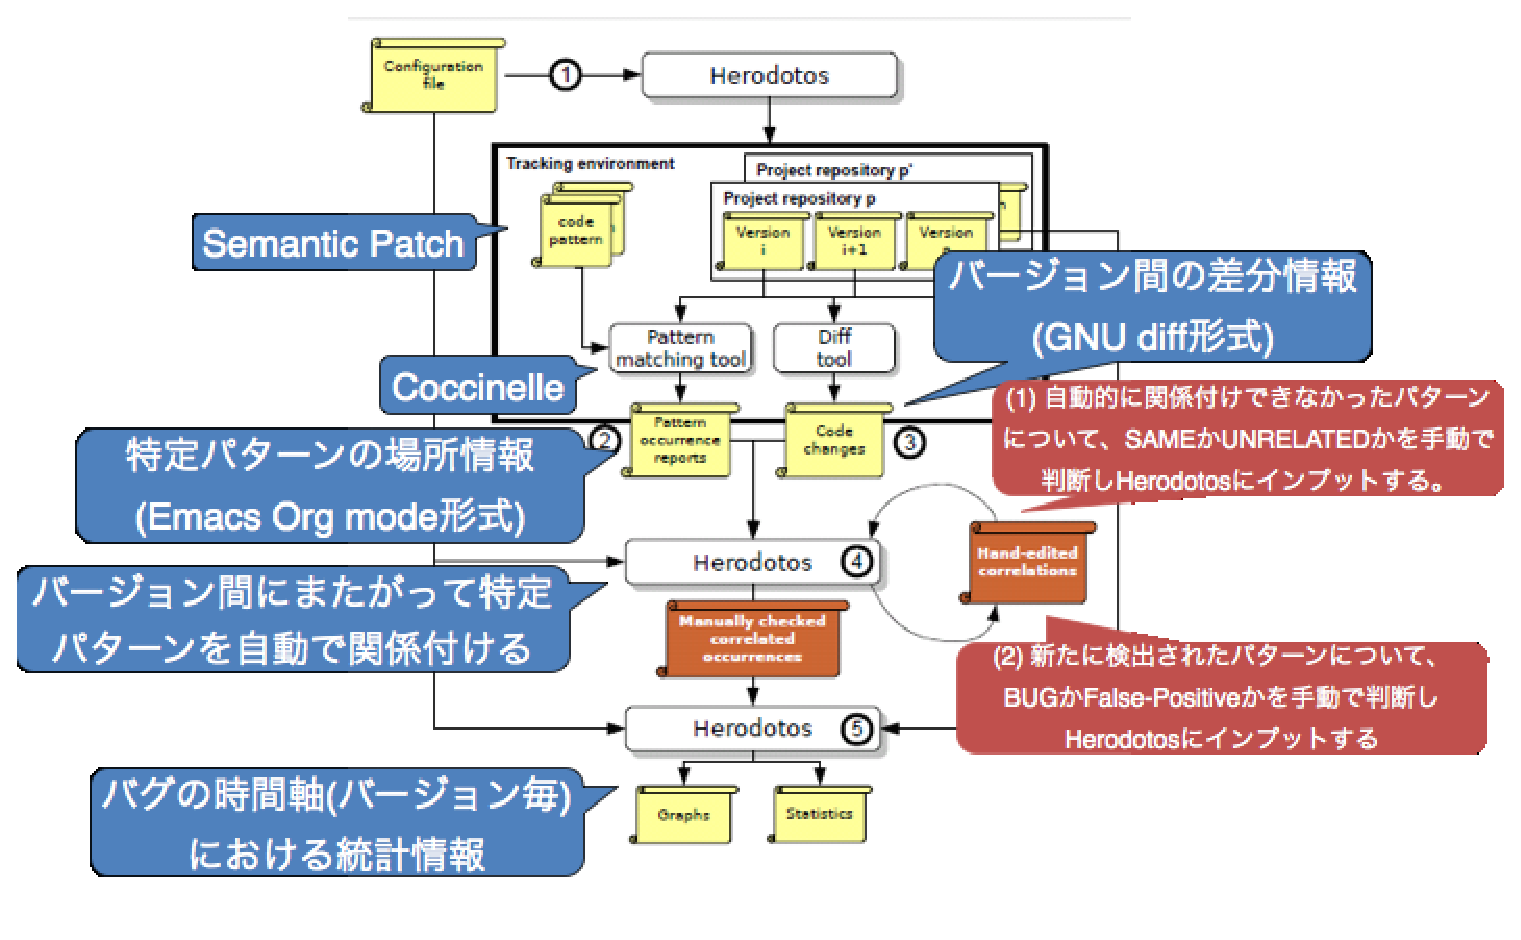
\includegraphics[width=\textwidth]{pic/heroview.eps}
  \caption{\acrshort{hero}のワークフロー}
  \label{heroview}
\end{figure}
\par
なお、\acrshort{cocci}に限らず一般に\acrshort{fp}を抑制する方法としては、使用するkernel configに基づいて無効な \verb|#ifdef| コードブロックを削除する前処理を行うことでビルド対象だけからなるソースコードを抽出し、検査対象となるソースコードそのものを絞るという方法も有りうる。この手法は\ref{mini}節で詳述する。
\subsubsection{Prequel}
\label{presec}
%\acrshort{pre}は\acrshort{cocci}と\acrshort{hero}と同じく\acrshort{inria}が開発中の、セマンティックパターンサーチをコミット履歴(パッチ)に対して行うツールである。
\acrshort{pre}はセマンティックパターンサーチをコミット履歴(パッチ)に対して行うツールで、\acrshort{cocci}と\acrshort{hero}と同じく\acrshort{inria}が開発している。
\acrshort{cocci}がソースコード空間に対してセマンティックパターンサーチを行うのに対して、\acrshort{pre}はサーチ対象を時間軸であるコミット履歴(パッチ)に拡張する。
\acrshort{pre}は開発中のためまだツールの実態は存在しないが、主に次の目的で利用されることが想定されている。
\begin{itemize}
  \item ある修正を行いたい場合に、過去に似たような修正が行われていないかを探すことでその適切な修正方法や副作用を調査する。
  \item 過去に行われた修正で現在のコードの別の箇所にも同じ修正を適用するべきパターンが残存していないかを探し、同じ問題が繰返し発生することを防止する。
  \item コミットログを解析し、各開発者に対するメトリクス(スキルレベルや危険なコードを書く可能性など)を測る。
\end{itemize}
\subsubsection{bugspots}
\acrshort{sil2linuxmp}で取り上げられた手法ではないが、\acrshort{pre}と関連してコミット履歴を元にバグ予測を行う手法に次のようなものが知られている。
\href{http://google-engtools.blogspot.sg/2011/12/bug-prediction-at-google.html}{Googleが2011年に公開したバグ予測アルゴリズム} \cite{google}によると、「バグ修正が最近頻繁にコミットされている箇所ほど残存バグがある可能性が高い」という経験則がある。
Googleでは毎日大量のコードコミットがあり人手によるレビューを全ての変更に対して十分に行うことは現実的に不可能であるため、バグがある可能性が高い"hot spot"に集中してレビューを行う必要がある。
そのようなhot spotを特定するために、trial \& errorの末に導かれた式が(\ref{google})である。
\begin{equation}
  Score = \sum_{i = 0}^{n} \frac{1}{1 + e^{-12t_{i} + 12}}
\label{google}
\end{equation}
\par
ここで、$n$はバグ修正に関連するコミットの数、$t_i$は$i$番目のバグ修正コミットのタイムスタンプでこの値は$0 \sim 1$で正規化されている。
$0$はソースコードベースで最初のコミットがあった時点を表し、$1$は現時点を表す。つまり式(\ref{google})を評価する時点によって$t_i$の値は変動する。
式(\ref{google})は新しいバグ修正ほど大きく重み付けされ、過去のバグ修正ほど小さく評価されるようスケーリングされている。
これをグラフに描くと図\ref{hotspot}のようになる。
\begin{figure}[ht]
  \centering
  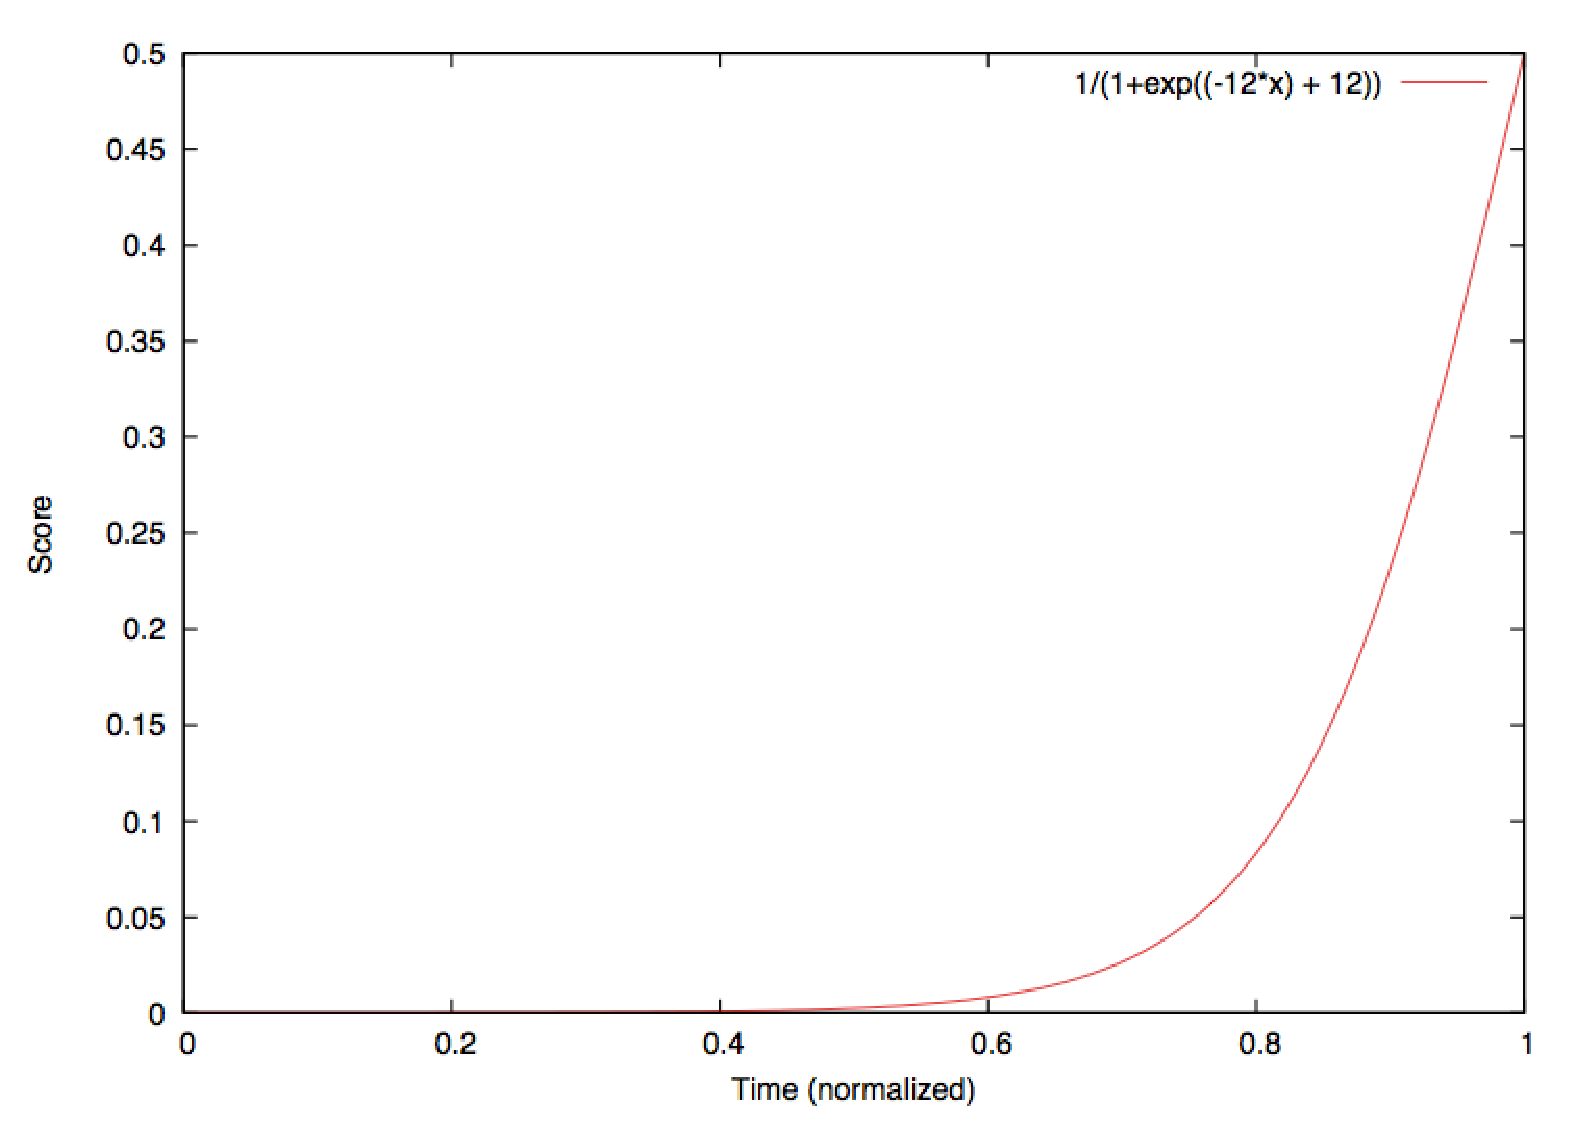
\includegraphics[width=0.8\textwidth]{pic/hotspot.eps}
  \caption{バグが残存する可能性が高いhot spotを評価する式(\ref{google})のグラフ}
  \label{hotspot}
\end{figure}
\par
式(\ref{google})の$Score$が一定の閾値を超える箇所に絞って集中的にコードレビューやコストのかかる検証を行うことで、ソフトウェアの品質を効率良く向上させることができる。
これはバグ修正のコミットタイミング情報のみを利用するごく単純な方法であるが、他のバグ予測アルゴリズムを抑えてバグの出現傾向を良く近似しているという。
\href{https://github.com/igrigorik/bugspots}{\acrshort{bugspot}} \cite{bugspot}はこのhot spot特定技法の\acrshort{rb}によるオープンソース実装である。
\newpage
\subsection{プロジェクト管理}
機能安全対応の開発においては開発対象のソフトウェアそのものに対する正当性検証に加えて、要求と設計のトレーサビリティなどマネジメント観点でのエビデンスを体系的に残し、開発プロセスが健全であることを認証機関に説明することも求められる。
次に\acrshort{sil2linuxmp}で採用が検討されているプロジェクト管理ツールを述べる。
\subsubsection{OGSN}
\label{ogsn}
\gls{gsn}は、達成すべき目的・性質・品質についてそのゴールを実現するための戦略・道筋・方法・思考を可視化するためのアシュアランスケース記法の一つである。
\acrshort{gsn}はEvidence Chainを記述するための国際的な標準表記法であり\acrshort{iso26262}で採用されている。
機能安全対応の際は特にSafety Case Conceptについて、思考の過程を共有し系統立てて議論を進め「なぜその方法で目的が達成できるのか」を認証機関に説明するために\acrshort{gsn}表記が用いられる。\\
 \href{http://blogs.itmedia.co.jp/hiranabe/2013/11/goal-structuring-network.html}{参考ブログエントリ:\acrshort{gsn}(Goal Structuring Notation)解説} \cite{gsne}
\par
\acrshort{gsn}表記は、長方形で示されたゴールが複数のサブゴールにブレークダウンされ、それらが最終的に円で示されたエビデンスまたはソリューションで支えられる構造を取る。
ゴール(長方形)とエビデンス(円)の間には戦略が平行四辺形で記述され、その戦略の根拠や仮定が楕円で、ゴールを目標として成立させている前提条件が角丸長方形で表現される(図\ref{gsn})。
\begin{figure}[ht]
  \centering
  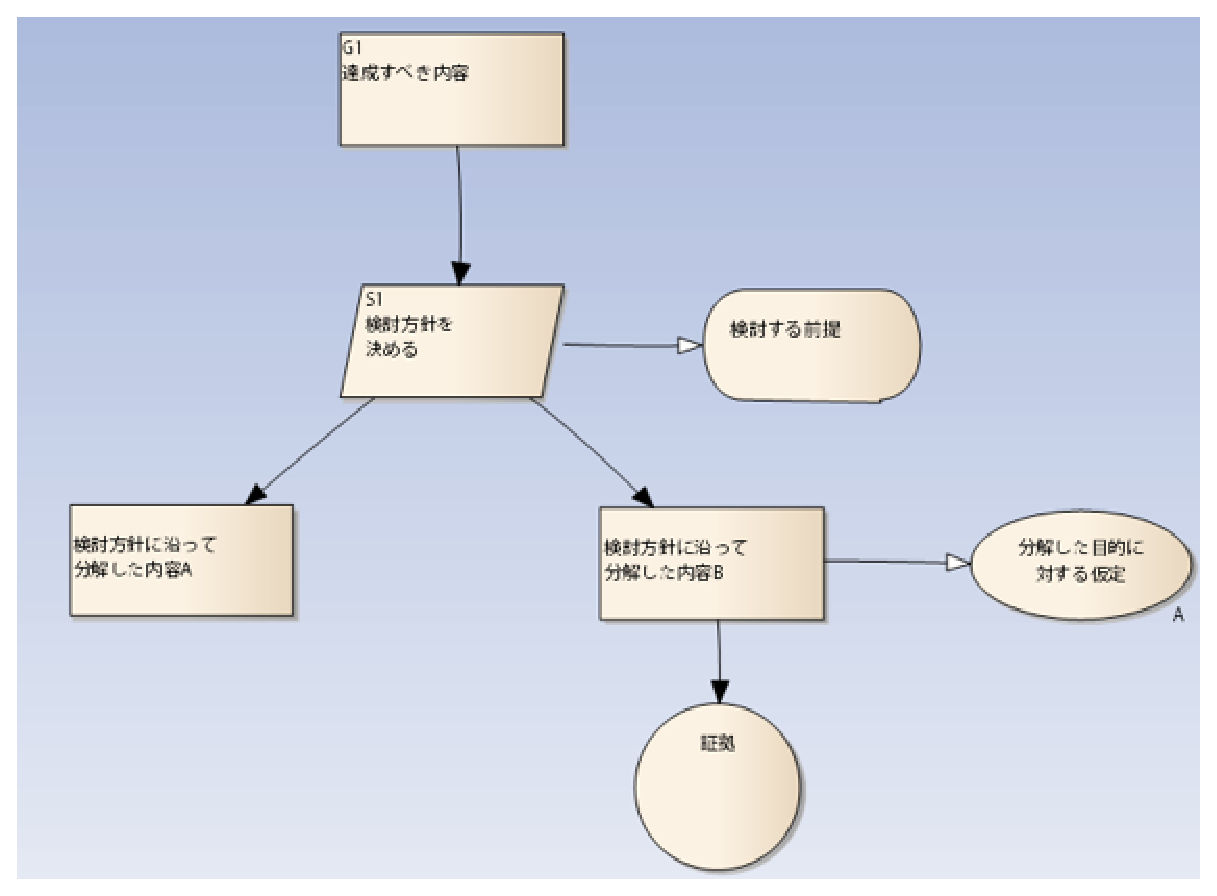
\includegraphics[width=0.9\textwidth]{pic/gsn.eps}
  \caption{\acrshort{gsn}表記の基本的な構造}
  \label{gsn}
\end{figure}
\par
\acrshort{sil2linuxmp}ではSafety Caseを\acrshort{gsn}表記で記述するためのエディタとして既存のツールが利用可能であるかが調査されたが、最終的に\acrshort{sil2linuxmp}プロジェクトで独自に\gls{ogsn}を開発することとなった。\acrshort{iec61508}-3 7.4.4.3 には、off-line 開発ツールの選定条件および選定根拠が明示されることとの記述がある。これに従い\acrshort{sil2linuxmp}では\acrshort{gsn}エディタに求めるマネジメント要件と機能要件として次の項目を挙げた。
\begin{itemize}
  \item マネジメント要件
  \begin{itemize}
    \item プロジェクトの初めから最後まで利用できることが保証されていること
    \item 様々な開発プラットフォーム上で利用可能であること
    \item 将来にわたっても利用できる実行できること
    \item オープンソースライセンスであること
  \end{itemize}
  \item 機能要件
  \begin{itemize}
    \item \acrshort{gsn}コミュニティが定める\href{http://www.goalstructuringnotation.info/documents/GSN\_Standard.pdf}{\acrshort{gsn}標準記法} \cite{gsn} Part1で定義された\acrshort{gsn}基本要素に対応していること
    \item \href{http://www.goalstructuringnotation.info/documents/GSN\_Standard.pdf}{\acrshort{gsn}標準記法} \cite{gsn} Annexes A1とB1の特に"Away Goal"表記に対応していること
  \end{itemize}
\end{itemize}
\par
上記で定めた要件をクライテリアとして、3つの\acrshort{gsn}エディタ\acrshort{dcase}、\acrshort{acedit}、\acrshort{advocate}が調査された。
\acrshort{gsn}エディタには商用で利用できるものが多数存在するが、それらはオープンソースライセンスでないため選定候補にはならない。
調査を行った既存の\acrshort{gsn}ツールと各々の特徴概要は次の通りであった。
\begin{itemize}
  \item \href{http://wiki.portal.chalmers.se/agda/pmwiki.php?n=D-Case-Agda.D-Case-Agda}{\acrshort{dcase}} \cite{dcase}
  \begin{itemize}
    \item \acrshort{eclipse}上で動く\acrshort{java}実装の拡張\acrshort{gsn}エディタ
    \item 厳密な\acrshort{gsn} standardに従っていない独自の表現がある
    \item 保守が止まっていて2010年の\acrshort{eclipse}でないと使えない
  \end{itemize}
  \item \href{https://code.google.com/p/acedit/}{\gls{acedit}} \cite{acedit}
  \begin{itemize}
    \item \acrshort{eclipse}上で動く\acrshort{java}実装の拡張\acrshort{gsn}エディタ
    \item \acrshort{dcase}よりも\acrshort{gsn}標準に従っている。
    \item \acrshort{eclipse}プラグインのインストールに難あり
  \end{itemize}
  \item \href{http://ti.arc.nasa.gov/m/profile/edenney/papers/sassur2012.pdf}{\acrshort{advocate}} \cite{advocate}
  \begin{itemize} 
    \item \acrshort{eclipse}上で動く\acrshort{java}実装の拡張\acrshort{gsn}エディタ
    \item グラフ要素の形が\acrshort{gsn}標準からかけ離れている
    \item \acrshort{eclipse}プラグインのインストールに難あり
    \item ホームページの最終更新が2011年
  \end{itemize}
\end{itemize}
\par
調査の結果、各ツールともメンテナンス状況が十分でないことと\acrshort{eclipse}に付随するバージョン・プラグイン依存関係が複雑であることから、\acrshort{sil2linuxmp}では既存ツールから適切なものを選定する方針を改め、独自にシンプルで必要最小限の\acrshort{gsn}エディタ\gls{ogsn}を開発することとなった。
\acrshort{ogsn}は120行程度の\acrshort{py}スクリプトであり、必要最小限の依存ライブラリ(ConfigParse, PyGraphviz)を持ち、\acrshort{gsn}グラフ表現では\acrshort{gv}を使用して自動的にノード・エッジを配置する仕組みとなっている。
\acrshort{ogsn}は\acrshort{sil2linuxmp}コアメンバーの\acrshort{ot}がプロトタイプを開発中で、今後は次の課題を中心に実装が進められる予定である。
\begin{itemize}
  \item \acrshort{gsn}標準記法の違反・例外チェック(ループ検出等)作りこみ
  \item \acrshort{gsn}標準で定められた記法の順次適用
  \item \acrshort{gsn}グラフ表示形式の洗練、Sub Treeの導入
  \item 複数分割ファイル入力のサポート
\end{itemize}
\subsubsection{rmToo}
\acrshort{sil2linuxmp}プロジェクトにおいて、開発履歴のトレーサビリティは\acrshort{git}で、目標(ゴール)からエビデンス・ソリューションへのトレーサビリティは\acrshort{ogsn}で確保されるが、これのみでは安全要求の開発履歴や要求間および要求と\acrshort{gsn}で表現した目標やソリューションとのトレーサビリティを取ることができない。
そこで\acrshort{sil2linuxmp}では\acrshort{gsn}エディタと同様にシンプルなオープンソースの要求管理ツールとして\href{http://rmtoo.florath.net}{\gls{rmtoo}} \cite{rmtoo}の使用が検討されている。
\par
\acrshort{rmtoo}は\acrshort{py}で実装されたシンプルなコマンドラインツールであり、Plain Textで書かれた要求事項からHTMLまたはPDF形式でのドキュメントや要求項目間の依存関係グラフを出力する。
\acrshort{rmtoo}には\acrshort{gui}や専用のエディタは付随しない。テキストベースの\acrshort{cui}ツールであるという特性は\LaTeX{}と親和性が高く、\acrshort{sil2linuxmp}の\gls{srs}文書は\LaTeX{}に\acrshort{ogsn}で描いた図と\acrshort{rmtoo}が併用されて要求間のトレーサビリティが考慮された構成となっている。
ツールの成熟度は高いが、\acrshort{rmtoo}がただ一人の開発者によって書かれていることと、\acrshort{gh}上の更新が2012年12月で止まっておりメンテナンス状況が不透明であることが懸念点として挙げられている。
\subsection{その他}
本節で詳しく述べることはしないものの、\acrshort{sil2linuxmp}で利用することが検討されているツール、または\acrshort{oss}・\acrshort{linux}開発において標準的に用いられているツールとして次のようなものがある。
\begin{description}
  \item[トレーシング・プロファイリング:]ftrace, kprobes, perf
  \item[カバレッジメトリクス測定:]gcov/lcov
  \item[ベンチマーキング:]lmbench, hackbench, crashme
\end{description}
\par
新たな開発ツールの採用を検討するときは、\ref{ogsn}項の\acrshort{gsn}エディタ選定で行ったようにツールに求める要件とクライテリアを定めて、各ツール候補についてアセスメントを行った上で適切なツールを選ぶ。
または要件を満たす既存ツールがなければ独自に新規開発を行う判断をする。
独自に新規開発を行う場合は、\acrshort{iec61508}が示す3通りの規格準拠方法(\pageref{3route}ページ)のうち$1_S$(初めから最後まで全て厳格に品質管理されたプロセスの下で開発・評価を行う)に従うことになる。
\newpage
\section{SIL2LinuxMPの戦略と規格準拠プロセスの理解}
\label{sil2process}
\ref{tool}節では、\acrshort{sil2linuxmp}プロジェクトでの利用が検討されているツール類のうち代表的なものを述べた。
本節では、機能安全対応開発においてツールセットを選択するための戦略と、既存ツールを組み合わせて新たなエビデンスを得る方法について\acrshort{sil2linuxmp}で検討されているアイディアを記載する。
\subsection{SIL2LinuxMPのツール選定戦略}
\label{toolselection}
\acrshort{sil2linuxmp}の開発基本方針はRoute \textbf{$3_S$}: assessment of non-compliant development(規格非適合の箇所に対して対策を行い適合と証明するに十分な根拠を与える)である。
このことは、従来の開発プロセスにおいて「設計・実装」に相当するフェーズが既存ソフトウェアの「選定」に置き換わるを意味している(図\ref{dlc})。
\begin{figure}[ht]
  \centering
  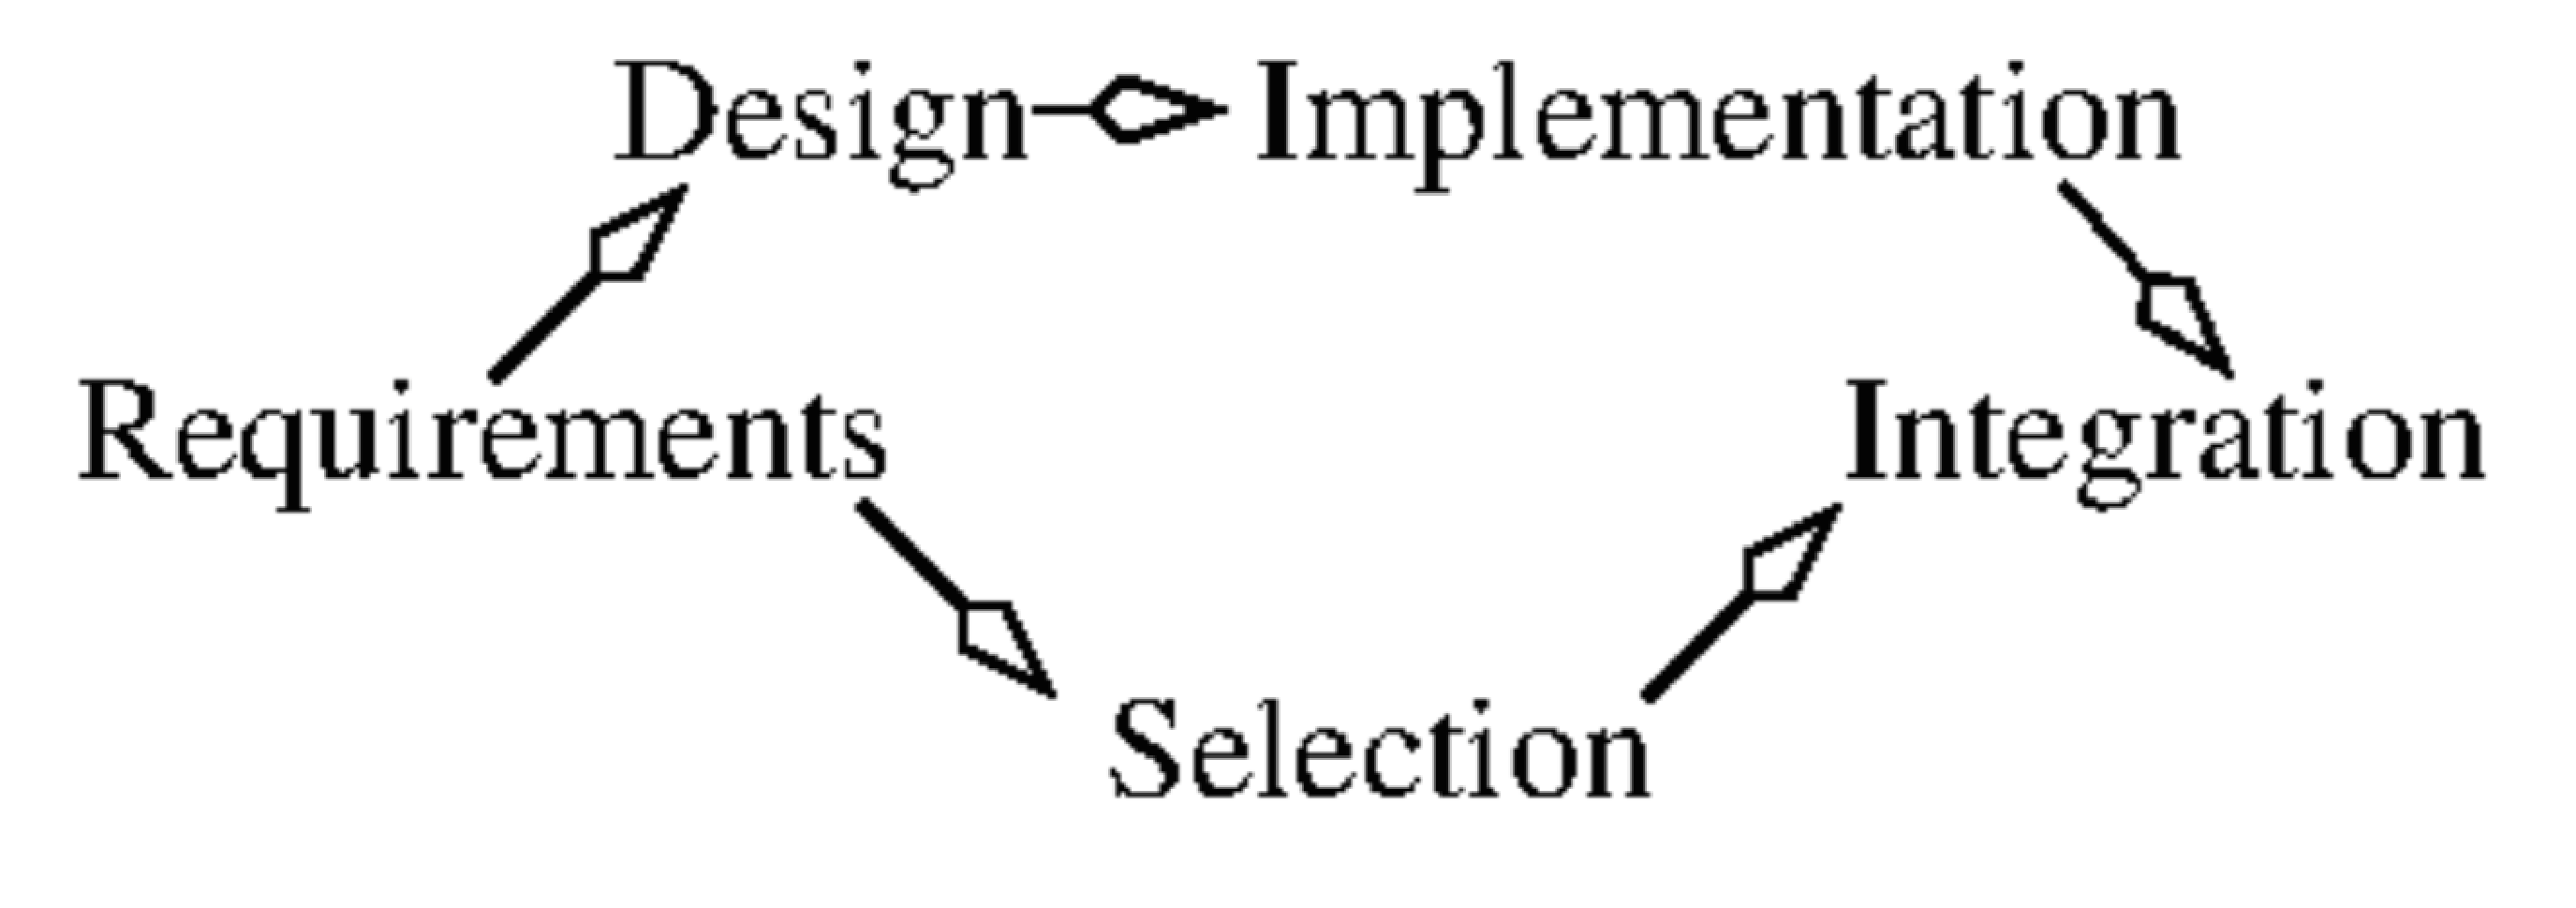
\includegraphics[width=0.7\textwidth]{pic/DLC.eps}
  \caption{既存ソフトウェアの選定プロセスが中心となる開発プロセスへの変化}
  \label{dlc}
\end{figure}
\par
選定フェーズの入り口ではソフトウェアに対する要求として選定クライテリアを定め、出口では定めたクライテリアに対する既存ソフトウェアのアセスメント結果を用意する。
既存ソフトウェアそれ自体が十分な品質・安全性を保証できない場合はそれを補うエビデンスを生成できる手段やツールを新たに導入する。
新たなツールの導入に関して特に考慮すべき事項は以下の通りである。
\begin{itemize}
  \item 非機能要件(実行環境・言語・依存ツール・使用方法)
  \item 機能要件(最低限備えるべき機能・あれば良い機能)
  \item カスタマイズの自由度
  \item コミュニティの成熟度と実績
\end{itemize}
\par
導入するツール自体についてもそれを採用する妥当性を認証機関に証明することが求められる。
ここでツール自体が多機能かつ大規模で複雑であったり、実行環境が特殊であったり、依存物が多かったりすると
精査しなければいけない対象と調査コストが現実的でない規模にまで膨らんでしまう。
そのため機能安全開発で使用するツールとしては、妥当性を証明できるほど十分に小さい構成と簡単な依存関係を持ち、かつ一般に広く認知されていて既に実績がある技術を使用したものが有利である。
\par
また新しいツール導入の際は、既に使用している開発ツールセットとの整合性もツール選定の基準となる。
同じ開発プラットフォーム上で動作するか、依存物の競合を起こさないか、バージョンの組み合わせは問題ないかなどを精査し、全体の開発ツールセットが「一貫した整合性を持つ必要最小限の構成」となるよう考慮する。
必要最小構成のツールセットを実現するためには、例えば使用しない機能を無効にすることでその部分の妥当性検証を省略する戦略が考えられる。
その場合は設定をオープンに操作できるカスタマイズ自由度があるツールほど有利である。
\subsubsection{スケールする検証フレームワークを実現するための戦略}
\label{scale}
\acrshort{sil2linuxmp}に特有の事情として、認証対象がオープンソースソフトウェアであるという点がある。
このことは、認証対象の妥当性を示すためのエビデンスを生成する検証ツールもオープンソースでなければならないことを意味する。
vendor lock-inを回避するため、かつ認証対象ソフトウェアのバージョンアップに追従するため、それらに対する検証は全てオープンな技術に基づいて開発者自身が実施できるものである必要がある。
このような要件に対応するためには何らかの検証自動化の工夫が不可欠である。
加えて、過去に実施したテストケースなどの資産を漸増的に繰返し再適用でき、さらにソースコードのアップデートに基づいて自動的にテストケースが追加生成されることで
その検証フレームワークを回せば回すほど自動的に品質を裏付けるエビデンスが蓄積されていくような仕組みを構築できれば、開発プロセスをスケールすることができる。
\ref{tool}節で述べたツールは各々、このような「スケールする検証フレームワーク」の一要素となる特性を持っている。
\acrshort{cocci}は過去に明らかになったバグを\acrshort{sm}で一般化・蓄積し回帰テストに用いることで同種のバグが新たに発生することを未然に防ぐことができる。
\acrshort{csmith}はランダムテストケースを生成し続けることでテスト母数を増やし品質の裏付けとなるエビデンスを蓄積することができ、
蓄積されたテストケースはソフトウェアのバージョンアップに対する回帰テストとして繰返し適用できる。
そして\acrshort{sil2linuxmp}では新たに\acrshort{fuzzer}の一種である\acrshort{syzkaller}の調査検討が進められているように、
「スケールする検証フレームワーク」を構築するためにはテストケースを自動生成できてそれを蓄積し回帰テストで繰返し適用できるような性質を持つ技術要素が特に有効であると考えられる。
\par
しかし図\ref{QA_Tasks}で述べた通り、品質管理ライフサイクルにおいてはテスト実行やテストケース生成にとどまらず、バグ抽出(\acrshort{fp}フィルタリング)、バグレポート生成、バグ管理、メトリクス測定・テストレポート生成など様々なタスクを実施する必要がある。
「スケールする検証フレームワーク」を構築するためには、これらのタスクを含めた品質保証エコシステム全体を自動化する工夫が必要となる。
特に問題となると考えられるのは「テストケース生成」と対になる「バグ抽出」の自動化である。
\acrshort{cocci}と\acrshort{csmith}の項目で述べた通り、これらは出力に大量の\acrshort{fp}が含まれるという共通の課題を持つ。
\acrshort{inria}が\acrshort{cocci}に対する\acrshort{fp}抑制策として\acrshort{hero}や\acrshort{pre}を提案しているが、これらはまだ人手の介入度合いが多く実績も少ない。
検証ツール全体を見渡しても、\acrshort{fuzzer}に代表されるテストケース生成自動化のためのツール・手法は豊富にあるものの、大量のテスト結果から真のバグをシステマティックに抽出する技法はほぼ存在しないように思われる。
テストケース生成を自動化した結果大量の\acrshort{fp}が出力され、その選別のために人手が必要である限り「スケールする検証フレームワーク」は実現できない。
テストケースを継続的に管理する仕組み構築に対して、テスト結果から真のバグを選別する何らかのバグトリアージの仕組みが不可欠である(図\ref{eco})。
\begin{figure}[ht]
  \centering
  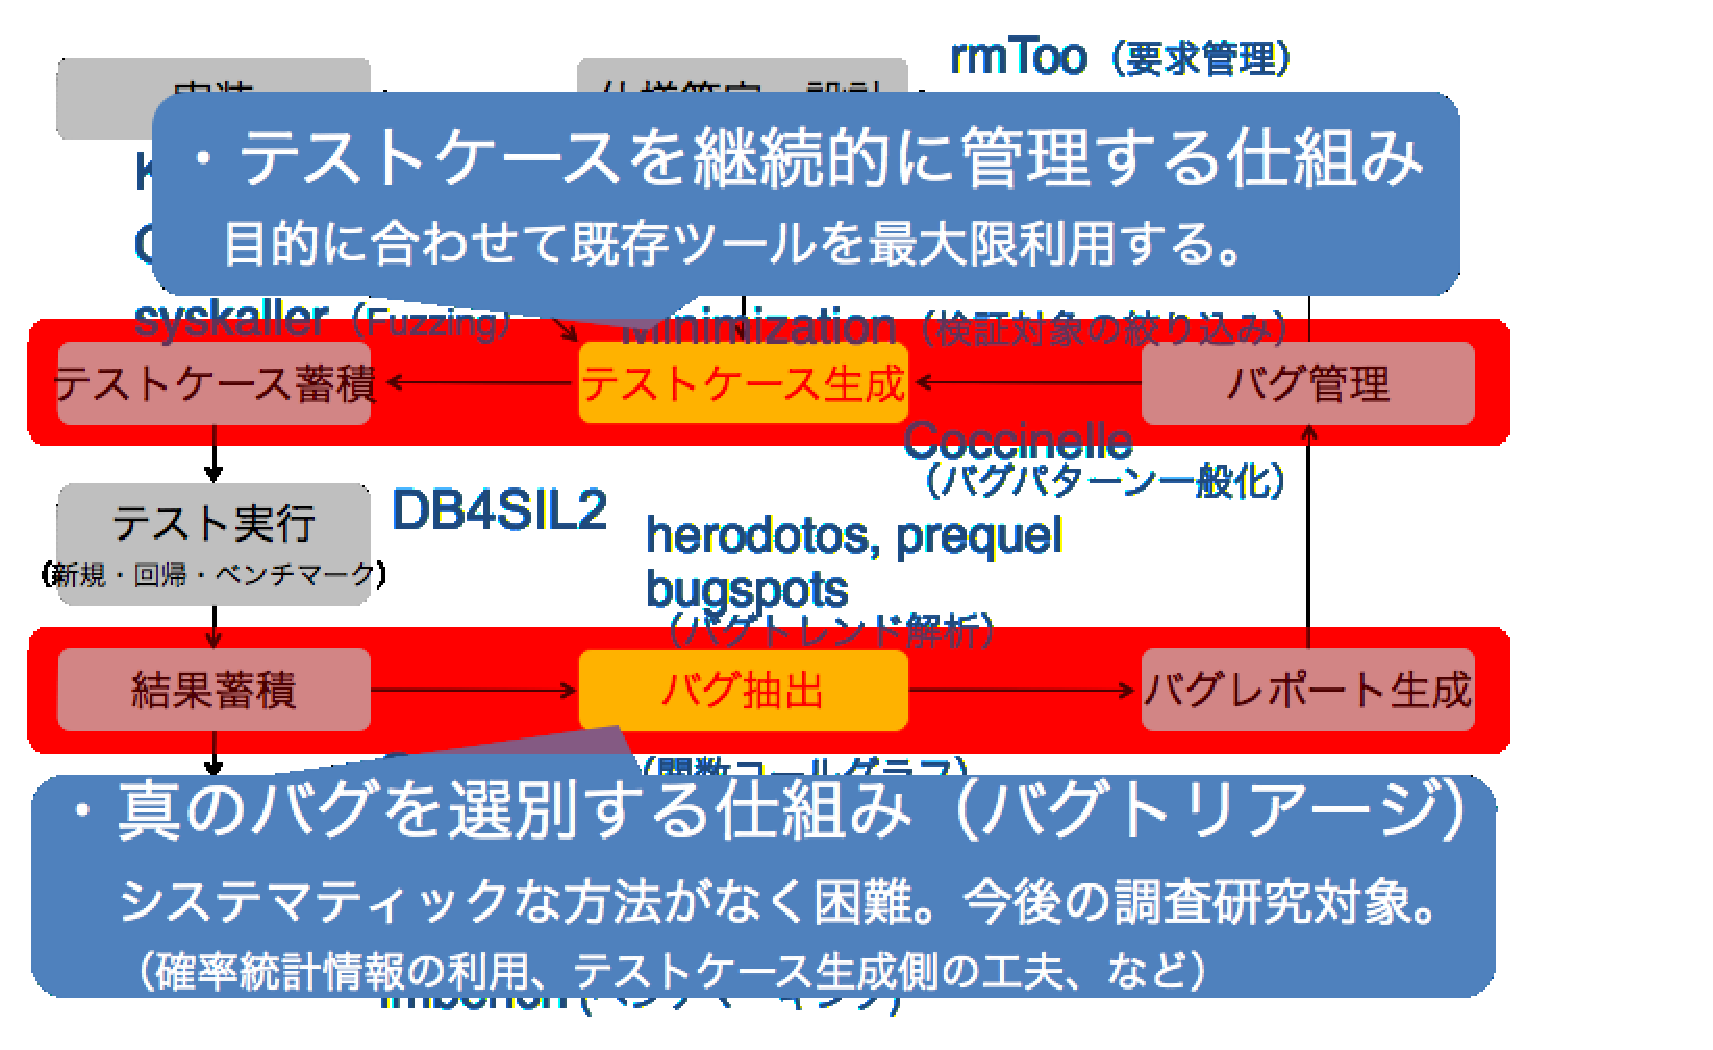
\includegraphics[width=0.95\textwidth]{pic/eco.eps}
  \caption{品質保証エコシステムにおいて対となるテストケース生成部分とバグ抽出部分}
  \label{eco}
\end{figure}
\par
バグトリアージという言葉は一般には「大量の不具合から優先して対処すべき案件を選別する」ことを意味するが、図\ref{eco}では「大量の\acrshort{fp}を含む不具合から真に不具合である案件を選別する」という拡張した意味で用いている。
テスト対象に応じて既存ツールから適切なテストケース生成ツールを選定するように、バグ抽出も対応の仕方はテスト結果の形式次第となる。
ただしここで場当たり的な\acrshort{fp}選別ではなく、\acrshort{bugspot}のように確率統計情報を用いて真のバグが残存する可能性が高い箇所を絞り込むことや、そもそも\acrshort{fp}を出力させない工夫をテストケース生成側で施すことなど、システマティックなバグトリアージ手法を確立する工夫が必要である。
具体的なバグトリアージ手法は今後の調査研究課題である。
\subsection{統合検証フレームワーク:DB4SIL2}
\label{db4sil2sec}
\acrshort{iec61508}-3 Table B.2 - Dynamic analysis and testing(図\ref{100})の7a$\sim$7dでは、各種カバレッジ$100\%$を達成することが\gls{sil2}で\gls{r}または\gls{hr}とされている。
ここで、カバレッジ測定のための技法は対象となるソフトウェアの特性に従って適切に選択されなければならない。
Table B.2の通り$100\%$カバレッジが達成できない場合はカバーできない箇所に対する合理的な説明を与えるか、カバーできない部分を特定し何らかの代替手段で補うことが求められている。
\begin{figure}[ht]
  \centering
  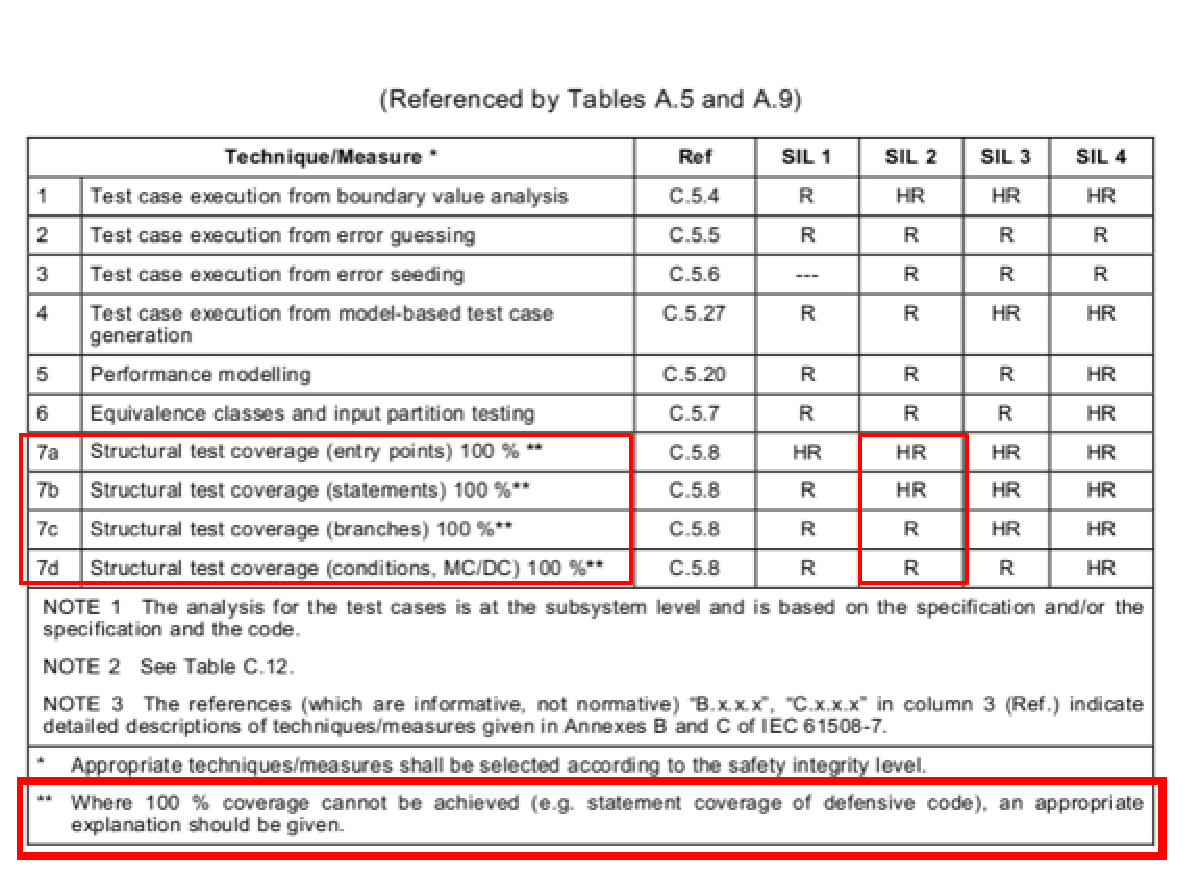
\includegraphics[width=\textwidth]{pic/100.eps}
  \caption{\acrshort{iec61508}-3 Table B.2 - Dynamic analysis and testing}
  \label{100}
\end{figure}
\par
一般にカバレッジを測定するテスト手法には、対象となる\acrshort{oss}ソフトウェアを開発するコミュニティで標準で使われている手法・ツールを用いる。
例えば\acrshort{linux} Kernelであれば\acrshort{ltp}や\acrshort{posix}を利用することをまず検討する。
その上で、既存の手法・ツールではカバーできない領域を特定し、そのようなコード領域へ何らかの対策を行う。
カバーされないコード領域への対策としては例えば次の\ref{enum:prove}, \ref{enum:makeup}ような戦略が考えられる。
\begin{enumerate}
  \item 該当コードが実行され得ないことを示してテスト不要であることを証明する \label{enum:prove}
  \item 該当コードをテストするテストケースを何らかの手段で生成する \label{enum:makeup}
\end{enumerate}
\par
戦略\ref{enum:prove}(テスト不要箇所の特定)の具体例としては、コンパイル対象とならないデッドコードを特定してそもそも検証対象から外す方法があり得る。
このデッドコードを除外する手法については\ref{mini}節で詳述する。
または、\acrshort{cpa}による形式検証手法により到達し得ないコードを特定して検証対象から外す根拠とすることも考えられる。
戦略\ref{enum:makeup}(テストケースの補完)については、例えば\acrshort{klee}による\acrshort{se}ツールで必要なカバレッジを達成するテストケースを(半)自動生成することが考えられる。
このように、コード内部構造の理解に基づいて\acrshort{black}テストのパフォーマンスを向上させる戦略は\textbf{\acrshort{gb}テスト}と呼ばれることがある。
\acrshort{sil2linuxmp}プロジェクトでは、\acrshort{gb}テストをはじめ\acrshort{oss}・\acrshort{linux}の機能安全対応に必要な検証技法を実装するための統合検証フレームワークとして\gls{db4sil2}を開発している。
\acrshort{db4sil2}の開発では、予め定められたクライテリアによって選定された検証ツールセットが統合され、ツール同士が入出力データをやり取りし互いにエビデンスを補完しあう形で図\ref{eco}のような品質保証エコシステムを構築することを目指している。
\begin{figure}[ht]
  \centering
  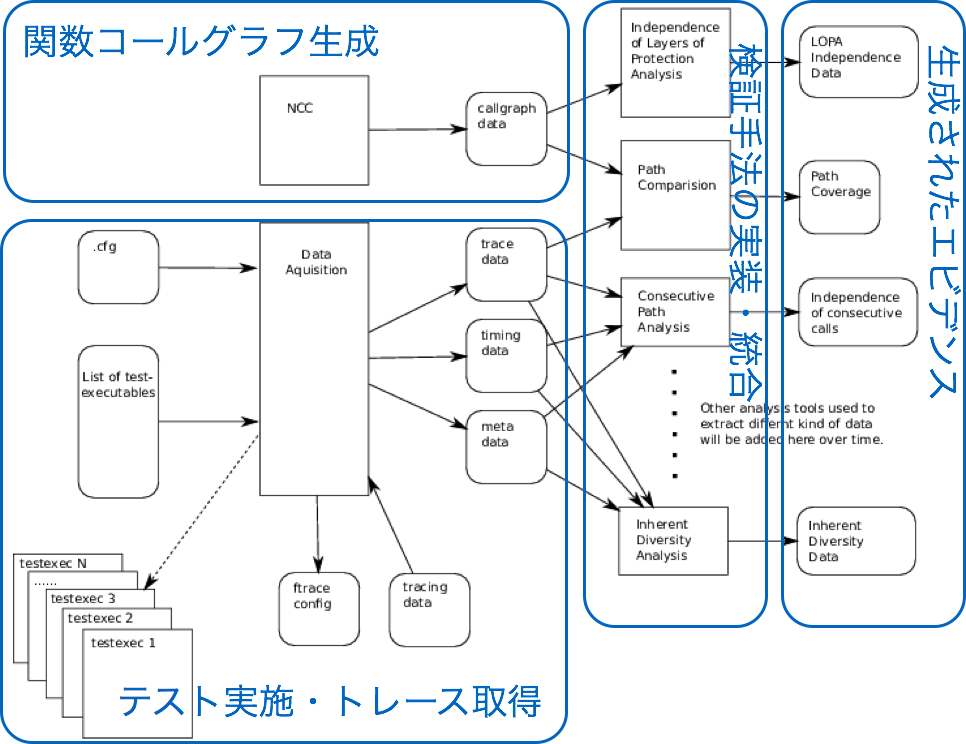
\includegraphics[width=\textwidth]{pic/db4sil2big.eps}
  \caption{\acrshort{db4sil2}の構想:機能安全認証に必要なエビデンスを生成する仕組みを実装・統合する}
  \label{db4sil2big}
\end{figure}
\par
図\ref{db4sil2big}は現時点での\acrshort{db4sil2}の構想である。\acrshort{db4sil2}は関数コールグラフやトレーサなど既存ツール
で得られるデータを入力とし、機能安全認証プロセスで求められる様々なエビデンスを生成する。以降で
は必要なエビデンスを得るために\acrshort{db4sil2}開発で具体的に検討されている検証手法を述べる。
\subsubsection{関数コールグラフとトレーサを用いたカバレッジ解析手法}
\label{callgraph}
\acrshort{gb}テストを行うためには、実施されたテストでカバーされていないコード領域を特定することが前提として必要である。
本章では、関数コールグラフとトレーサを用いてカバレッジ解析を行う手法として\acrshort{db4sil2}開発で検討されている戦略を述べる。
\begin{figure}[ht]
  \centering
  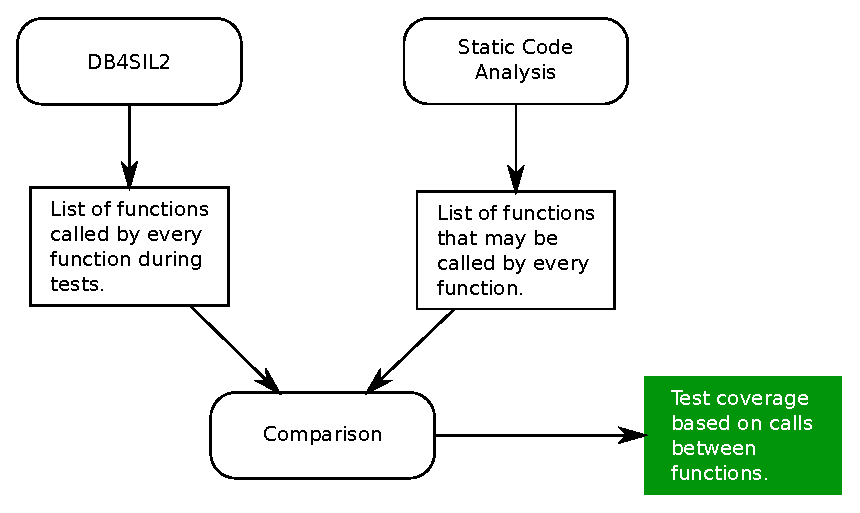
\includegraphics[width=0.85\textwidth]{pic/cov.eps}
  \caption{関数コールグラフとトレーサを用いたパスカバレッジ測定方法}
  \label{cov}
\end{figure}
\par
図\ref{cov}は、事前にソースコードの静的解析によって得られた関数コールグラフと、テストによって得られた動的トレース結果を付き合わせることでパスカバレッジに関するメトリクス解析を行うワークフローである。
ここで、静的関数コールグラフを得るためには\ref{cv}項で記載した\acrshort{cv}を使用する。
\acrshort{cv}のnccを使い関数ポインタを介した呼び出し関係までを静的に解析することで、対象とするソースコードにおいて実行される可能性のある関数呼び出しパスを全てリストすることができる。
動的トレースの取得には\gls{ftrace}を用いる。\acrshort{ftrace}は、kernel空間の動的挙動に対するデバッグや障害・性能解析ツールとして広く使われている\acrshort{linux} Kernelの機能であり、
予め埋め込まれたトレースポイントを契機として関数呼び出し履歴と各々の関数の実行時間を低負荷で記録することができる。
ここで、実行され得る関数呼び出し関係を\acrshort{cv}を使いソースコードを基に全て洗い出した上で、そのソースコードでビルドしたソフトウェアで任意の動的テストを行ったときの関数呼び出し履歴を\acrshort{ftrace}で取得することを考える。
これによって得られた静的関数コールグラフと動的関数コールグラフを比較した結果、静的グラフに存在するが動的グラフには出現しない関数呼び出しパスが特定されれば、そのパスが実施されたテストでカバーされていない部分であると言うことができる。
また、その比較解析結果から関数呼び出しパスについてのカバレッジメトリクスを測定することができる。
\par
例えば、システムコール\verb|SyS_sched_getscheduler()|を契機に呼ばれる可能性のある関数は\acrshort{cv}の関数コールグラフ導出により明らかになる(図\ref{getscheduler})。
ここで、あるテストを行った結果\acrshort{ftrace}によるトレースが図\ref{getscheduler}中のTrace1, Trace2のように得られたとする。
Trace1, Trace2中で現れた関数呼び出しパスをコールグラフ中で探すと、コールグラフで\checkmark{}を付けたエッジが見つかる。
\checkmark{}を付与していないエッジがカバーされていない関数呼び出しパスに相当する。
\begin{figure}[ht]
  \centering
  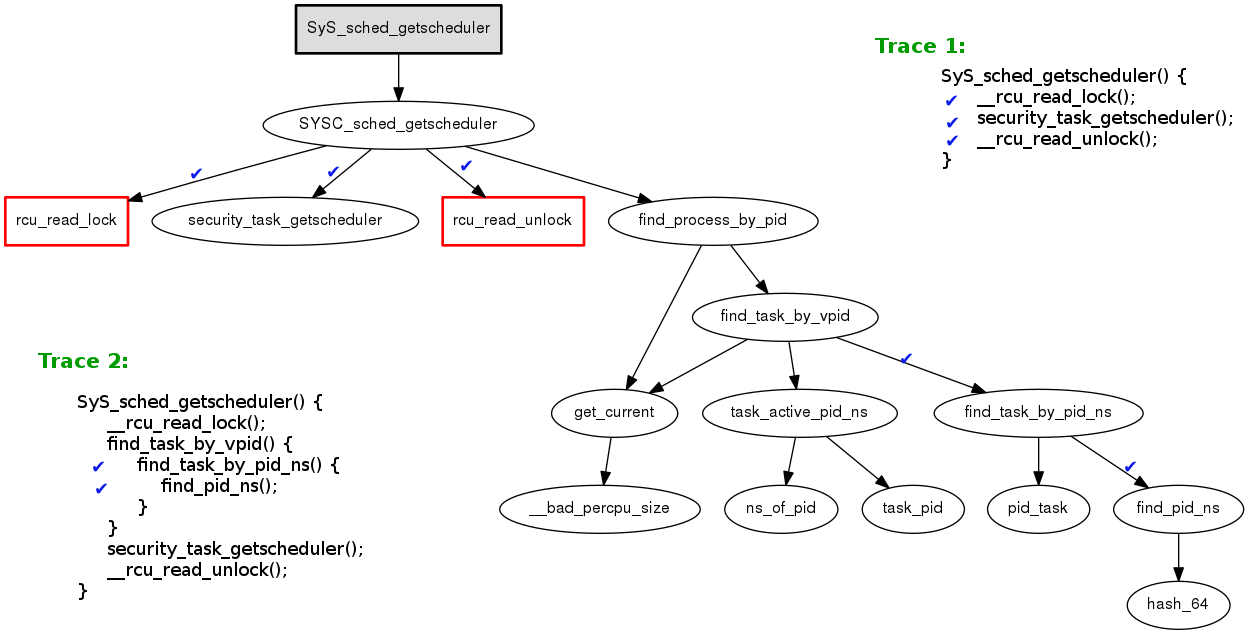
\includegraphics[width=\textwidth]{pic/getscheduler.eps}
  \caption{関数コールグラフとトレーサを用いたパスカバレッジ測定例}
  \label{getscheduler}
\end{figure}
\par
本項で述べた解析手法によって得られ得た静的・動的関数コールグラフは、ソースコードに変更が入った際にその全体への影響を調べるインパクトアナリシスにとっても有用なデータとなる。
変更が加えられた関数を直接・間接的に呼んでいる関数、または変更箇所から呼ばれている関数が既に明らかであれば、変更の全体への影響を調べるためには関数コールグラフ上変更箇所と関係を持つコード領域のみに注目してレビューや回帰テストを実施すればよい。
データを介したやり取りや、イベント・割り込みが関わる直接的な関数呼び出しでない非同期挙動の分析はこの限りではないが、インパクトアナリシスの範囲を考えるための一つの指標として用いることができる。
\par
以上のような関数コールグラフとトレーサを用いたカバレッジ測定手法およびインパクト解析手法は、\acrshort{ftrace}の性質上適用できる範囲がカーネル空間のみに制約される。
しかし\acrshort{sil2linuxmp}プラットフォームとして\acrshort{sil2}対応の目標となっている領域には\acrshort{linux} Kernelに加えて\acrshort{bb}と\acrshort{glibc}からなる最小構成のユーザ空間も含まれる。
そのため、同様の手法をユーザ空間でも適用するべきであると\acrshort{sil2linuxmp}コミュニティでは認識されており、
ユーザ空間における具体的ツールと実現手段は今後の調査検討課題となっている。
\subsubsection{関数コールグラフのLOPAへの応用}
\label{sil0}
機能安全対応のシステム開発では、必ずしも常にシステム全体に同一の安全水準が求められるわけではない。
システム要求や開発リソース・コストなどのマネジメント戦略次第で、特定の部分のみ\acrshort{sil2}水準の安全性を確保しその他の部分は\acrshort{sil0}(\gls{qm}:安全性の要求なし)領域とするアーキテクチャ設計も可能である。
ただし、このように複数の安全水準を持つサブシステムを混在させる場合は各領域の影響が互いに干渉することのないように対策を施さなければならない。
特に\acrshort{sil0}(\acrshort{qm})非安全領域で欠陥や障害があった場合にその影響が\acrshort{sil2}安全領域に伝搬することは許容されない。
\acrshort{sil2}安全領域と\acrshort{sil0}(\acrshort{qm})非安全領域との隔離を実現する手段のひとつとして、\acrshort{sil2linuxmp}では図\ref{isol}のように\acrshort{linux}コンテナ技術を利用した構成が検討されている。
\begin{figure}[ht]
  \centering
  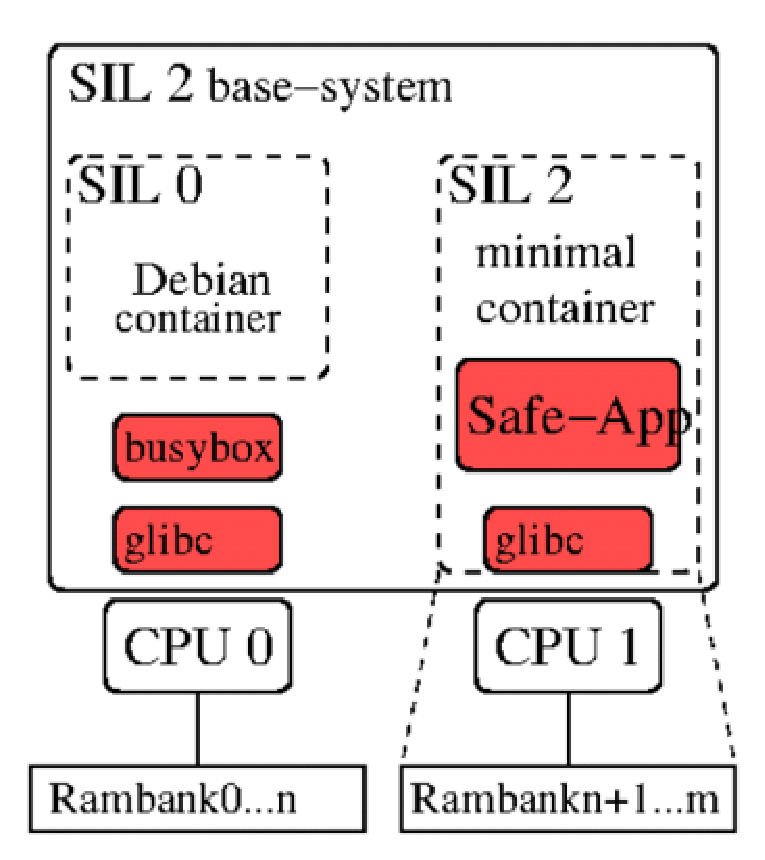
\includegraphics[width=0.45\textwidth]{pic/isol.eps}
  \caption{\acrshort{sil2}安全領域と\acrshort{sil0}(\acrshort{qm})非安全領域をコンテナで隔離するシステム構成}
  \label{isol}
\end{figure}
\par
\acrshort{gnu}/\acrshort{linux}システムにおける一般的なコンテナ技術はユーザ空間から見たリソースを各々のコンテナ内で隔離するものであるが、厳密にkernel内部のリソースまで隔離して運用することはできない。
そのため、本来安全に隔離保護されているべき領域に対するリスク評価を行う\gls{lopa}の実施が求められる。
\acrshort{sil2linuxmp}では\acrshort{db4sil2}開発の一環として、関数コールグラフを利用した\acrshort{lopa}実施方法が次のように検討されている。
%\paragraph{ \acrshort{seccomp}と\acrshort{cgroups}のリソース独立性を解析する例}
%\par
\subsubsection{\acrshort{seccomp}と\acrshort{cgroups}のリソース独立性を解析する例}
\gls{cgroups}はプロセスのリソース(CPU、メモリ、ディスクI/O等)の利用を制限または隔離する\acrshort{linux} Kernelの仮想化機能である。
\gls{seccomp}はユーザ空間に対してシステムコールの利用を制限したサンドボックス環境を提供する\acrshort{linux} Kernelのセキュリティ機能である。
\acrshort{cgroups}と\acrshort{seccomp}はともに、ユーザ空間のアプリケーションを隔離することで他のアプリケーションやシステムにその挙動の影響を伝搬させないことを意図して使われることが一般的である。
互いにその挙動が独立であることが想定されているならば、各々の機能から使われる関数も呼び出し関係は分離されているはずであると予想される。
ここで、\acrshort{cgroups}と\acrshort{seccomp}の両方の機能を無効にしたときに使われるコード領域に含まれる関数の集合を$BASE$、
\acrshort{seccomp}だけを有効にしたときの領域に含まれる関数の集合を$SEC$、
\acrshort{cgroups}だけを有効にしたときの領域に含まれる関数の集合を$CGR$として各々の関係を考える(図\ref{bs})。
\begin{figure}[ht]
  \centering
  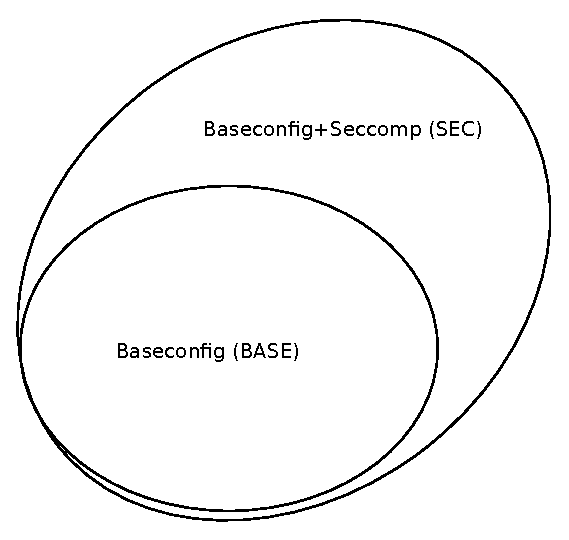
\includegraphics[width=0.6\textwidth]{pic/bs.eps}
%  \caption{\acrshort{seccomp}機能を有効にしたときのコード領域\verb|SEC|と\verb|SEC|に無関係なベース領域\verb|BASE|}
  \caption{\acrshort{seccomp}機能を有効にしたときに使われる関数の集合$SEC$と、無効にしたときの関数の集合$BASE$}
  \label{bs}
\end{figure}
\par
\acrshort{seccomp}機能と\acrshort{cgroups}機能が独立であるならば$SEC$と$CGR$の共通部分は$BASE$の部分集合であるはずであるが、$SEC$と$CGR$の共通部分に属しかつ$BASE$に属さない関数
%\newline
($ \in (SEC \cap CGR) \smallsetminus BASE$)が存在する(図\ref{intersec})。
このような共通部分に属する関数は、各々\acrshort{seccomp}機能と\acrshort{cgroups}機能に関する関数コールグラフを導出することで調べることが可能である。
\acrshort{seccomp}と\acrshort{cgroups}から共通して使われる関数が特定されれば、それらの共通関数に範囲を限定してレビューや検証のコストを集中させることで各々の機能の独立性を効率的に調査することができる。
つまり本項で述べた戦略は機能の挙動が完全に隔離されていることの証明を目指すのではなく、各々から共通して参照される範囲を特定した上で
その限定された部分が共通して参照されても問題ないことを示すかまたは必要に応じて何らかの対策を施すという、
\acrshort{iec61508}-3 7.4.2.12 Route $3_S$: assessment of non-compliant development の原則に基づくものである。
\begin{figure}[ht]
  \centering
  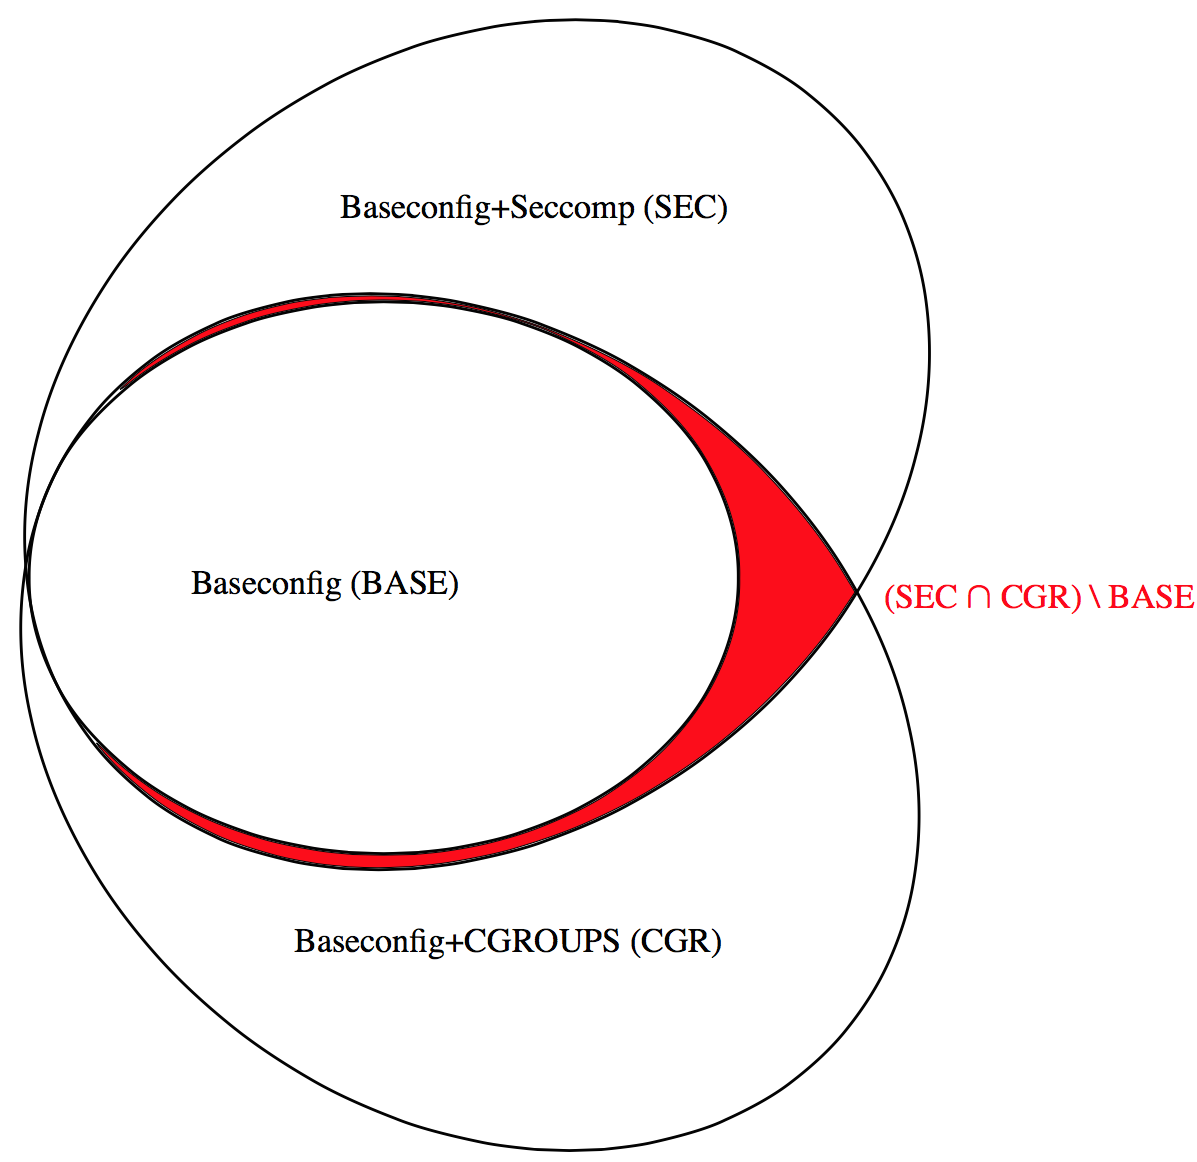
\includegraphics[width=0.8\textwidth]{pic/intersec.eps}\
  \caption{$(SEC \cap CGR) \smallsetminus BASE \neq \varnothing$}
  \label{intersec}
\end{figure}
\subsubsection{\acrshort{seccomp}と\acrshort{cgroups}の\gls{ccf}分析例}
ソフトウェアの開発履歴情報を共通原因故障(\gls{ccf})分析に応用することが\acrshort{sil2linuxmp}プロジェクトで検討されている。
ソースコードの記述スタイルは各プロジェクト毎に方針が存在し統一されていることが多いものの、コードには開発者毎に思考の癖や好みのパターンが表れる。
そのような開発者依存のコーディングパターンがあるロジック実装で使われたりある別のパターンと併用されたりした場合に
何らかの問題を引き起こす原因となることがあり得る。
オープンソースソフトウェアの開発には\acrshort{git}に代表されるバージョン管理システムが使われることが一般的であり、
そこにはソースコード変更の単位でその開発者名が記録されている。
ここで、例えば\acrshort{seccomp}プロジェクトの\acrshort{git}コミット履歴から\acrshort{seccomp}プロジェクトに参加している開発者を調べれば、
\acrshort{cgroups}プロジェクト側で発生したバグの原因となるコードを書いた開発者が\acrshort{seccomp}のコードにもコミットした履歴があるかどうかが分かる。
この情報を手掛かりにして、\acrshort{cgroups}プロジェクトのバグと同じ原因で発生する可能性のあるバグが\acrshort{seccomp}プロジェクトにも残存する可能性をさらに分析することができる。
\par
ちなみに\acrshort{seccomp}と\acrshort{cgroups}の両方のプロジェクトにコミット履歴を残している開発者と各コミット数は表\ref{deveopers}の通りである。
\begin{table}[hb]
  \caption{\acrshort{seccomp}と\acrshort{cgroups}に共通する開発者と各コミット数}
  \label{deveopers}
  \centering
  \begin{tabular}{ll|ll}
    \multicolumn{2}{c|}{\acrshort{seccomp}} & \multicolumn{2}{c}{\acrshort{cgroups}} \\
    \hline 
    54 & Linus Torvalds & 2 & Linus Torvalds \\
    52 & Daniel Borkmann & 203 & Daniel Borkmann \\
    48 & David Howells & 3 & David Howells \\
    2 & Fabian Frederick & 1 & Fabian Frederick
  \end{tabular}
\end{table}

\section{質疑や議論を通したSIL2LinuxMPコミュニティへのコントリビューション}
本節では、2015年4月からこれまで\acrshort{sil2linuxmp}活動を通してコミュニティへ働きかけた内容を記載する。
\acrshort{sil2linuxmp}プロジェクトにおける主なコミュニケーション手段はメーリングリストと\acrshort{git}である。
プロジェクトに対する活動は各参加者の主体性に任されている状況であり、全ての活動はメーリングリストおよび\acrshort{git}の履歴に残り
最終的に\acrshort{sil2linuxmp}の成果として参照される。
このようなオープンなプロジェクトでは、有益なコントリビューションを多く残している参加者ほどコミュニティに認知される。
\ref{contribution}節で述べたように、近年はオープンなコミュニティで認知されること自体が長期的に価値のある投資としての意味を持つ。
\acrshort{oss}に対する機能安全のノウハウを得るという目的と並んで、日立の\acrshort{sil2linuxmp}への貢献を示すため、
また筆者自身が\acrshort{oss}活動の進め方を理解するため、研修期間を通してメーリングリストと\acrshort{git}での活動を活発に行うことを意識した。
\subsection{メーリングリスト上での活動}
\label{mailinglist}
\href{http://lists.osadl.org/pipermail/sil2linuxmp/}{\acrshort{sil2linuxmp}メーリングリスト} \cite{mail}はコミュニティでの議論や何らかの告知が行われる公な場である。
日立からは、\gls{srs}などの\acrshort{sil2linuxmp}ドキュメントとコンプライアンスルートおよび各種検証手法の不明点の質問をするため、また日立が行った技術調査・検討内容の報告をするめにメーリングリストへの投稿を継続的に行った。
表\ref{mailindividual}は、メーリングリストへの投稿者別に2015年4月$\sim$ 2016年3月までの投稿数が多い順で投稿者メールアドレスをリストした結果である。
日立は4名から投稿があり、そのうち筆者(kotaro.hashimoto.jv@hitachi.com)は36投稿でプロジェクト全参加者中で2番目に投稿数が多かった。
1、3番目に投稿数が多いder.herr@hofr.at (Nicholas Mc Guire)とandreas.platschek@opentech.atは\acrshort{sil2linuxmp}プロジェクトの主催メンバである。
これまでこのメーリングリストでは、日立が発した質問に対してNicholasやAndreasが回答しそれに他の参加者が反応して議論が膨らんでいく、という形式で話が進むケースが多かった。
\begin{table}[H]
  \caption{個人別\acrshort{sil2linuxmp}メーリングリスト投稿数ランキング(2015年4月$\sim$ 2016年3月)}
  \label{mailindividual}
  \centering
  \begin{tabular}{l|l}
    \multicolumn{1}{c|}{投稿数} & \multicolumn{1}{c}{投稿者メールアドレス} \\
    \hline 
    40 & der.herr@hofr.at (Nicholas Mc Guire) \\
    \textbf{36} & \textbf{kotaro.hashimoto.jv@hitachi.com} \\
    16 & andreas.platschek@opentech.at (andi@opentech.at 含む) \\
    15 & Mandar.Pitale@bmw-carit.de \\
    13 & julia.lawall@lip6.fr \\
    \textbf{13} & \textbf{krishnaji@hitachi.co.in} \\
    12 & C.Emde@osadl.org \\
    8 & Lukas.Bulwahn@bmw-carit.de \\
    7 & georg.schiesser@opentech.at (george.schiesser@gmail.com 含む) \\
    6 & Bernhard.Noelte@tuev-sued.de \\
    3 & office@osadl.org \\
    2 & Georg.Waibel@sensor-technik.de \\
    2 & KaziKhaled.Al-Zahid@bmw-carit.de \\
    2 & Tilmann.Ochs@bmw.de \\
    1 & Ursula.Braun@osadl.org \\
    1 & Tilmann.Ochs@bmw-carit.de \\
    \textbf{1} & \textbf{masami.hiramatsu.pt@hitachi.com} \\
    1 & Quirin.Gylstorff@kuka.com \\
    1 & dvhart@linux.intel.com \\
    1 & khoroshilov@ispras.ru \\
    \textbf{1} & \textbf{pradyumna@hitachi.co.in} \\
    1 & Kai-Daniel.Niestroj@sensor-technik.de \\
    1 & Christian.Hartmann@kuka.com \\
    1 & jeremiah.foster@pelagicore.com \\
    1 & Mandar.Pitale@bmw.de
  \end{tabular}
\end{table}
\par
表\ref{mailcompany}は投稿者のメールアドレス情報を元に企業別で投稿数を集計した結果である。
日立は\acrshort{sil2linuxmp}プロジェクト主催元の\acrshort{ot}に続いて51投稿で、プロジェクト全参加企業中で2番目に投稿数が多かった。
\begin{table}[H]
  \caption{企業別\acrshort{sil2linuxmp}メーリングリスト投稿数ランキング(2015年4月$\sim$ 2016年3月)}
  \label{mailcompany}
  \centering
  \begin{tabular}{l|l}
    \multicolumn{1}{c|}{投稿数} & \multicolumn{1}{c}{投稿者メールアドレス} \\
    \hline 
    63 & opentech.at (hofr.at 含む) \\
    \textbf{51} & \textbf{hitachi.com} (hitachi.co.in 含む) \\
    29 & bmw.de (bmw-carit.de 含む) \\
    16 & osadl.org \\
    13 & lip6.fr (\acrshort{inria}) \\
    6 & tuev-sued.de \\
    3 & sensor-technik.de \\
    2 & kuka.com \\
    1 & pelagicore.com \\
    1 & linux.intel.com \\
    1 & ispras.ru
  \end{tabular}
\end{table}
\par
表\ref{thread}はメーリングリストでの話題(スレッド)別に各話題における投稿数を集計した結果である。
これらのうち、日立が初めに投稿した質問または提案で議論が始まったものは右端に\checkmark{}を付けている。
\begin{table}[H]
%  \footnotesize
  \small
  \caption{スレッド別\acrshort{sil2linuxmp}メーリングリスト投稿数ランキング(2015年4月$\sim$ 2016年3月)}
  \label{thread}
  \centering
  \begin{tabular}{l|l|l}
    \multicolumn{1}{c|}{投稿数} & \multicolumn{1}{c|}{スレッドタイトル名(の一部)} & \multicolumn{1}{c}{日立の投稿で議論が始まったもの} \\
    \hline 
    \textbf{19} & \textbf{Question about SRS and verification strategy} & \checkmark{} \\
    16 & Return Oriented Programming (ROP) & \\
    11 & Next SIL2LinuxMP meeting in September & \\
    \textbf{10} & \textbf{How could we qualify a toolchain (T3 off-line} & \checkmark{} \\
    \textbf{10} & \textbf{SRS question: How will COTS upgrade process be} & \checkmark{} \\
    \textbf{10} & \textbf{Pruning function call graph} & \checkmark{} \\
    \textbf{8} & \textbf{Gray box Analysis approach} & \checkmark{} \\
    8 & Preliminary safety concept available? & \\
    \textbf{8} & \textbf{Results of Static analysis on Minimized source code} & \checkmark{} \\
    7 & sil2linuxmp & \\
    7 & Scheduliing of Application & \\
    \textbf{7} & \textbf{SRS question: SIL0 isolation} & \checkmark{} \\
    \textbf{6} & \textbf{Scoping targets for Tracing and Coverage} & \checkmark{} \\
    \textbf{6} & \textbf{Live DVD build issue} & \checkmark{} \\
    5 & Addressing the differences between ISO 26262 and IEC &  \\
    5 & SIL2Linux Meeting in July 2015 (2015-07-22) at &  \\
    \textbf{5} & \textbf{Minimal kernel source code [SIL2LinuxMP scope]} & \checkmark{} \\
    \textbf{4} & \textbf{Minimal SIL2LinuxMP configuration} & \checkmark{} \\
    \textbf{4} & \textbf{Questions about Live-DVD and OGSN regarding} & \checkmark{} \\
    \textbf{4} & \textbf{Question about purpose of the Prequel} & \checkmark{} \\
    \textbf{4} & \textbf{Comparison between static call graph and dynamic} & \checkmark{} \\
    3 & Route 3s: Detailed Design, & \\
    \textbf{3} & \textbf{How OSS licenses should be handled with} & \checkmark{} \\
    \textbf{3} & \textbf{Is the "Device Tree" SIL2LinuxMP target component} & \checkmark{} \\
    2 & First CM Report 2015-05-20 & \\
    \textbf{2} & \textbf{SIL2LinuxMP tool needs for Graybox process} & \checkmark{} \\
    2 & Welcome Hitachi! (and pull request for d5bcaad0) & \\
    2 & Third CM Report 2015-08-15 & \\
    2 & 4th CM Report 2015-09-16 & \\
    2 & iso from Live DVD & \\
    2 & Target kernel version/configuration in SIL2LinuxMP & \\
    2 & Initial Test & \\
    2 & Second CM Report 2015-07-01 & \\
    2 & Pull request for branch lbulwahn (commit 5671424 & \\
    1 & SIL2 Project Plan V1.4 with final list of & \\
    1 & Welcome Hochschule Heilbronn! & \\
    1 & Reminder: SIL2LinuxMP Progress Meeting on September & \\
    1 & Network connectivity to the GIT repository & \\
    1 & SIL2Linux MP Milestone Meeting will take place on & \\
    1 & [GIT PULL] Please pull dvhart: doc make target & \\
    1 & SIL2LinuxMP Milestone Conference (Go/No-Go) on & \\
    1 & Agenda of the SIL2LinuxMP Milestone Conference & \\
    1 & SIL2LinuxMP Live DVD now live on the Internet & \\
    1 & SIL2LinuxMP Meetings Schedule & \\
    1 & Shadow monitoring at the OSADL QA Farm & \\
    1 & FOSDEM 2016 -- safety-critical talk in Brussels? & \\
    1 & Web-based command line access to the SIL2LinuxMP & \\
    1 & 5th CM Report 2016-03-01 & \\
    1 & Reminder: Review of current SIL2LinuxMP & \\
  \end{tabular}
\end{table}
\par
表\ref{thread}を見ると、実質半数以上の議論が日立からのメーリングリスト投稿を契機で行われていることが分かる。
日立の投稿により行われた議論は主に以下に示す話題に関するものであった。
%の\ref{enum:mailfirst}$\sim$\ref{enum:maillast}に示す話題に関するものであった。
\begin{itemize}
  \item コンパイラの検証手法(\ref{compveri}項で記載)\label{enum:mailfirst}
  \item \acrshort{db4sil2}の目的と\acrshort{gb}テストの定義・手法(\ref{db4sil2sec}節で記載)
  \item 関数コールグラフを導出するツール調査(\ref{cv}項で記載)
  \item 関数コールグラフを利用したカバレッジ測定手法(\ref{callgraph}項で記載)
  \item デッドコードを削除し検査対象を限定する\acrshort{codemini}技法(\ref{mini}節で記載)
  \item \acrshort{codemini}技法を応用し関数コールグラフを小さくする手法(\ref{minigraph}項で記載)
  \item \acrshort{sil2linuxmp}プラットフォームの検証で使われるツール選定(\ref{toolselection}項で記載)
  \item \acrshort{git}コミット履歴をソフトウェア品質測定に測定する手法(\ref{presec}項で記載)
  \item \acrshort{cocci}の機能安全プロセスにおける使用方法(\ref{cocci}項で記載)
  \item 安全領域と非安全領域の独立性分析方法(\ref{sil0}項で記載)
  \item \acrshort{sil2linuxmp}開発環境(\acrshort{dvd})のインストール不具合対策
  \item \acrshort{ogsn}不具合対策
  \item デバイスツリーの機能安全対策
  \item 機能安全認証プロセスと\acrshort{oss}ライセンスチェックの関係
  \item 機能安全対応開発におけるチーム構成と役割定義
  \item \acrshort{oss}コンポーネントのアップデートプロセス
  \item \acrshort{linux} Kernelの最小構成設定の作成方法 \label{enum:maillast}
\end{itemize}
\par
\acrshort{sil2linuxmp}メーリングリスト上の活動を通して、\ref{tool}節や\ref{sil2process}節で記載したような一連のノウハウを得ることができたほか、
\acrshort{sil2linuxmp}コミュニティを巻き込んで議論を行うことができた。
特に\acrshort{sil2linuxmp}プロジェクトの参加企業が20社以上ある中で、レビューパートナーである日立が率先して質疑応答や意見交換を行ってきたことは
\acrshort{sil2linuxmp}コミュニティに対する貢献として十分なアピール効果があったと考えている。
ただし表\ref{mailcompany}に示す通り、プロジェクト主催者である\acrshort{ot}と日立以外の参加企業の活動形跡がほとんど見えない状況であることが大きな懸念である。
プロジェクト2年目に入る2016年4月以降では、\acrshort{ot}と日立以外の参加企業も活発かつ自主的にプロジェクトに参加していくことができるような
何らかのマネジメント対策が早急に必要である。
%\newpage
\subsection{\acrshort{git}上での活動}
\acrshort{sil2linuxmp}プロジェクトはドキュメントやツールの開発トレーサビリティを確保するために\acrshort{git}を構成管理ツールとして使用している。
日立は、\acrshort{sil2linuxmp}プロジェクトで独自に開発されるツールのテストやデバッグに参加することを通して、
レビューパートナーとして有益なフードバックを行うことを目標とした。
また、各種検証ツールの調査結果の共有や日立が開発した\acrshort{codemini}ツール(\ref{mini}項で記載)の公開も\acrshort{git}上で行った。
\subsubsection{\acrshort{sil2linuxmp}が開発するツールへのフィードバック}
\acrshort{sil2linuxmp}プロジェクトが独自に開発をするツール類には以下のものがある。
\begin{description}
  \item [\acrshort{dvd}:]\acrshort{sil2linuxmp}活動を行うための統合開発環境。\acrshort{dl}で作成される。
  \item [\acrfull{ogsn}:]\ref{ogsn}項で記載。
  \item [\acrshort{db4sil2}:]\ref{db4sil2sec}項で記載。
\end{description}
\par
\acrshort{dvd}は、\acrshort{sil2linuxmp}で選定または開発されたツールセットが予めセットアップされた統一環境を提供することを目的に作成される。
\acrshort{sil2linuxmp}開発環境のベースとしては\acrshort{deb}がNicholasらによるアセスメントにより選定されている。
日立は\acrshort{dvd}のイメージビルドからシステム起動までをテストし、見つかった手順上の不備について各々対策方法を調査してビルドスクリプトおよび手順の修正をコミットした。
\acrshort{ogsn}についてもスクリプトと手順がまだ成熟しておらず、インストールが成功しない問題や例外処理が多数不足している等の課題があった。
\acrshort{ogsn}を初めて導入する開発者が手間取ることのないように、日立は手順およびスクリプトの整備を行った。
関連して、\acrshort{ogsn}と連携している\acrshort{srs}等のドキュメントにも\LaTeX{}コンパイル上の問題があったためドキュメントの生成スクリプトに対する修正を行った。
\subsubsection{検証ツール調査内容の共有}
\acrshort{sil2linuxmp}計画においてはじめの1年間は技術調査フェーズと位置づけられており、各種検証ツールの調査とそれらの機能安全対応開発での使用方法検討が重視されていた。
テストカバレッジ測定方法の検討(\ref{callgraph}項)において、当初NicholasとAndreasら(\acrshort{ot})は関数コールグラフ生成ツールとして\acrshort{cflow}を試用していた。
しかし\acrshort{cflow}には関数ポインタを介した呼び出し関係を表現できないという欠点や、関数名や変数名の扱いに関して\pageref{cv_vs_cflow}ページで述べたような不備があった。
そこで日立は独自に調査を行い、\acrshort{cflow}の欠点を補いかつトレーサと併用してカバレッジ測定に用いるという目的に適切な関数コールグラフ生成ツールとして
\acrshort{cv}が利用できることを\acrshort{sil2linuxmp}メーリングリスト上で報告した。
またその調査実験結果の詳細報告を\acrshort{git}レポジトリにコミットした。
\subsubsection{日立が独自に開発した検証手法やツールの公開}
\acrshort{sil2linuxmp}活動の一環で日立が独自に開発した技法として、
ソースコード中でコンパイル対象とならない無効な \verb|#ifdef| コードブロックを削除することで
使用されるコードだけを抽出し検査対象となる範囲を限定する\acrshort{codemini}がある(\ref{mini}項で詳述)。
\acrshort{codemini}のソースコード、試用手順、応用例、技術検討内容の公開を\acrshort{sil2linuxmp}プロジェクトの\acrshort{git}レポジトリ上で行った。
\par
また\acrshort{sil2linuxmp}ドキュメント開発において、複数のドキュメントで共通して用いられる用語を一箇所のファイルでまとめて記載し
各々のドキュメントから参照する形で管理するための、大規模な\TeX{}ファイルの修正が行われたことがあった。
この作業を促進するため、各\TeX{}ファイル中でまだ用語が直接記載されている箇所を特定して要修正箇所としてハイライトするスクリプトを作成し\acrshort{sil2linuxmp} \acrshort{git}レポジトリ上で公開した。
\subsubsection{\acrshort{sil2linuxmp} \acrshort{git}レポジトリでの活動結果}
\acrshort{sil2linuxmp} \acrshort{git}レポジトリ上で日立が作成または編集したファイルとその内容は次の通りであった。
\begin{itemize}
  \small
  \item \verb|doc/investigation/Analysis_tools/callgraphs/CodeViz/CodeViz_investigation_note.txt| \\
        $\cdots$ 関数コールグラフ生成ツール\acrshort{cv}の調査
  \item \verb|doc/investigation/Analysis_tools/callgraphs/CodeViz/fix_callback_traversing.patch| \\
        $\cdots$ \acrshort{cv}付属のコールグラフデータ視覚化スクリプトの関数ポインタ周りの不具合修正
  \item \verb|doc/investigation/Analysis_tools/callgraphs/CodeViz/ncc_visualization.txt| \\
        $\cdots$ \acrshort{cv}のnccにより生成したコールグラフデータの表示方法に関する調査
  \item \verb|doc/investigation/Analysis_tools/callgraphs/CodeViz/vfs_read.png|
  \item \verb|doc/investigation/Analysis_tools/callgraphs/CodeViz/vfs_write.png| \\
        $\cdots$ \acrshort{cv}で生成した関数コールグラフの例
  \item \verb|src/tools/minimization/minimize.py| \\
        $\cdots$ 使用されないコードを削除して検証範囲を限定する\acrshort{codemini}技法の実装
  \item \verb|src/tools/minimization/README.md| \\
        $\cdots$ \verb|minimize.py|の説明書
  \item \verb|src/tools/minimization/EvaluationNote| \\
        $\cdots$ \acrshort{bb}に\verb|minimize.py|を適用したときのソースコード複雑度測定実験
  \item \verb|pm/weekreports/khashimoto/March_2016| \\
        $\cdots$ \acrshort{cv}で生成する関数コールグラフと、\acrshort{codemini}適用後に\acrshort{cflow}で生成したグラフのサイズ比較調査
  \item \verb|doc/investigation/Analysis_tools/callgraphs/PruningCallGraph.txt| \\
        $\cdots$ \acrshort{codemini}技法で関数コールグラフを枝刈りする応用例
  \item \verb|pm/weekreports/khashimoto/2015-12-16_LiveDVD_SetUp_Note| \\
        $\cdots$ \acrshort{dvd}ビルド手順の不具合修正調査
  \item \verb|src/tools/live-dvd/build.sh| \\
        $\cdots$ \acrshort{dvd}ビルド手順の不具合修正
  \item \verb|src/investigation/ogsn/ogsn3.py| \\
        $\cdots$ \acrshort{ogsn}の例外処理強化
  \item \verb|src/investigation/ogsn/README| \\
        $\cdots$ \acrshort{ogsn}のインストール・使用手順不備の修正
  \item \verb|pm/weekreports/khashimoto/2015-12-15_OGSN_rmToo_Installation_Note| \\
        $\cdots$ \acrshort{ogsn}および\acrshort{rmtoo}を併用して\acrshort{srs}ドキュメントを生成するための手順調査
  \item \verb|pm/pm_docs/SRS/Makefile| \\
        $\cdots$ \acrshort{srs}ドキュメントを生成するための\LaTeX{}、\acrshort{rmtoo}、\acrshort{ogsn}統合手順不具合修正
  \item \verb|share/SIL2Linux_Abbreviations.tex| \\
        $\cdots$ \acrshort{sil2linuxmp}用語集の表記誤り修正
  \item \verb|src/tools/acroscan/acroscan.py| \\
        $\cdots$ \TeX{}ファイル中にハードコーディングされている用語を検出して参照形式で書き換えるよう修正を促すツール
  \item \verb|src/tools/acroscan/README| \\
        $\cdots$ \verb|acroscan.py|の説明書
\end{itemize}
\par
上記の変更は全て\acrshort{sil2linuxmp} \acrshort{git}レポジトリの本線に取り込まれている。
ただし、\acrshort{sil2linuxmp}構成管理チームは各々のプロジェクト参加者のブランチの内容までレビューしているわけではなく、
コミットメッセージの形式的な確認のみを行ってマージを行っている状況である。
今後は\gls{ccb}が設置されて、変更内容をきちんとレビューした上でマージ判断を行うプロセスが導入される予定である。
\par
図\ref{gitstats}は、2015年4月から2016年3月までに行われた\acrshort{git}コミットについて寄与率(Commits(\%))が多い順で開発者をリストした結果である。
\acrshort{git}コミットの集計には\href{http://gitstats.sourceforge.net/}{\acrshort{gitstats}} \cite{gitstats}を用いた。
\begin{figure}[ht]
  \centering
  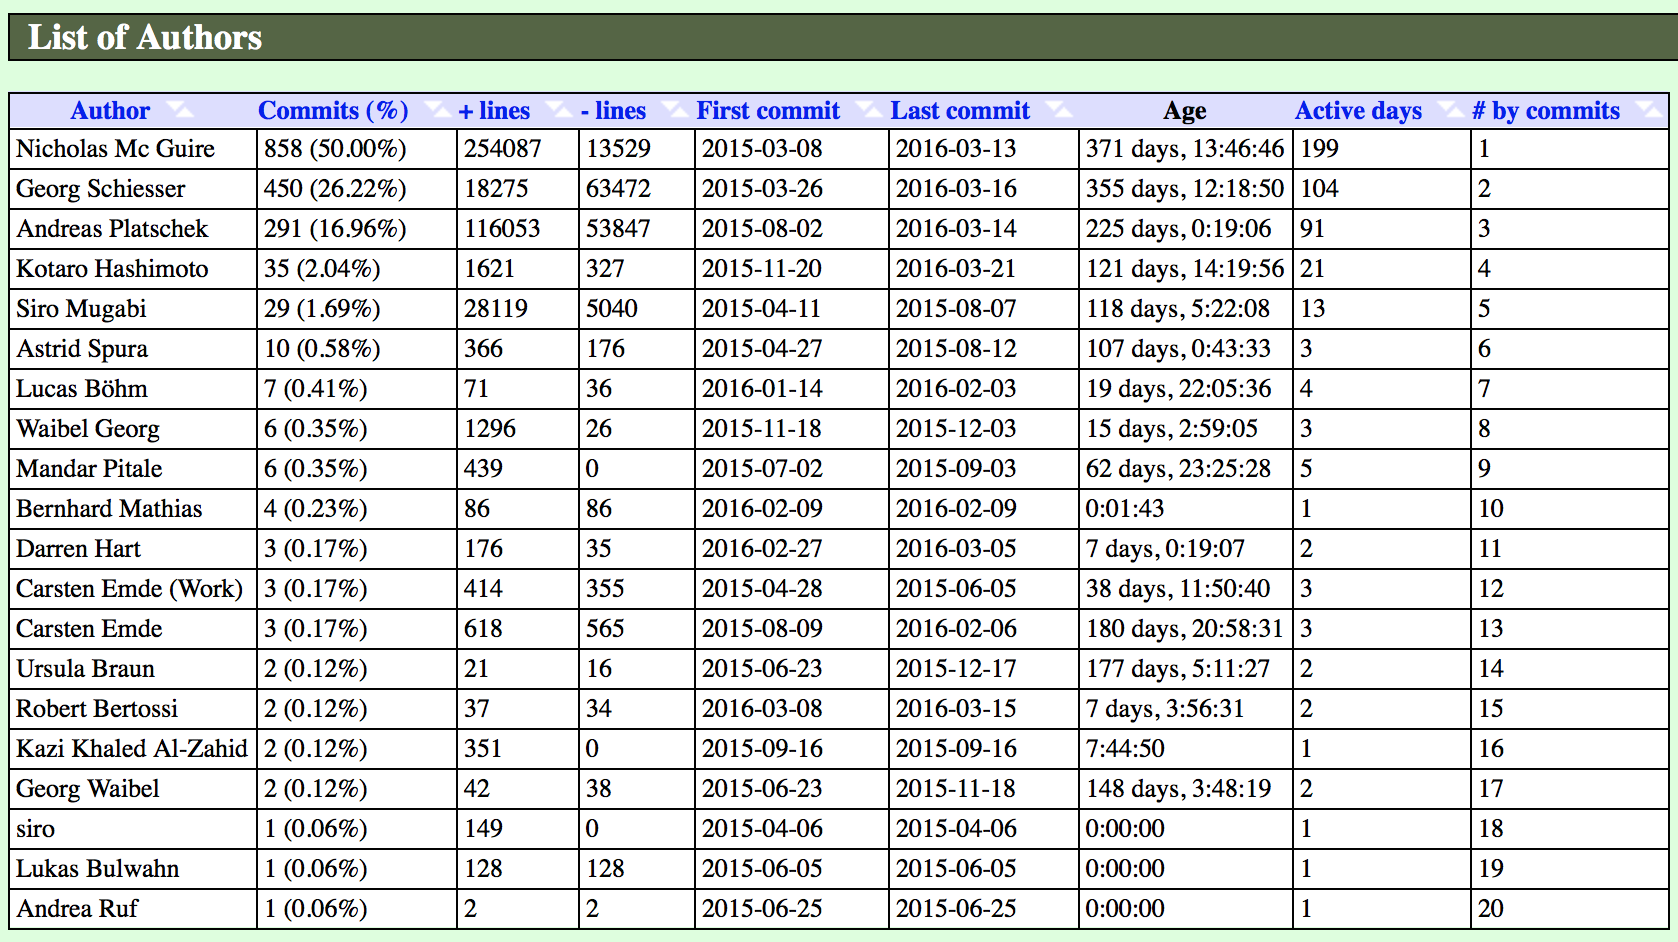
\includegraphics[width=\textwidth]{pic/gitstats.eps}
  \caption{開発者別\acrshort{sil2linuxmp} \acrshort{git}コミット寄与率集計結果}
  \label{gitstats}
\end{figure}
\par
コミット寄与率Top3のNicholas Mc Guire, Georg Schiesser, Andreas Platschekは\acrshort{sil2linuxmp}を主催する\acrshort{ot}のメンバーで、ドキュメント執筆、ツール調査・開発を主導している。
筆者(Kotaro Hashimoto)は35コミット(2.04\%)で、\acrshort{ot}メンバに続き4番目に寄与率が大きかった。
\ref{mailinglist}項でも述べたとおり、\acrshort{ot}と日立以外の参加企業からのコミットが非常に少ないことがプロジェクト上の懸念である。
今後\acrshort{sil2linuxmp}プロジェクトを盛り上げるために日立としてできる対策を考え、コミュニティが自発的に動き出すような仕掛けをしていくことがプロジェクト成功に不可欠である。
\subsection{Face to face meeting}
\acrshort{sil2linuxmp}プロジェクトは参加者間のコミュニケーションルートとしてメーリングリストと\acrshort{git}の他にface to face形式のミーティングやワークショップを重視している。
2016年3月第二週にはドイツ・ハイデルベルグでプロジェクト参加者全員を対象とするマイルストンミーティングが行われた。
ここでは\acrshort{sil2linuxmp}プロジェクトが始まってから約1年となるタイミングで、これまでの進捗と成果・残課題の共有および2年目の方針についての議論が行われた。
この場で日立からは\acrshort{codemini} Strategyと題した技術発表を行った。
\acrshort{codemini}技法は既存の様々なソフトウェア検証・解析手法のパフォーマンスを向上させる可能性を持ち、
機能安全認証プロセスにとっても非常に有効な戦略となり得る技術として\acrshort{sil2linuxmp}コミュニティから高い評価を受けた。
ミーティング終了後には\acrshort{ot}と日立とで別途会合を行い、より突っ込んだ質疑応答や意見交換を行った。
マイルストンミーティングでは、これまでメールと\acrshort{git}だけを介してコミュニケーションを取ってきた技術者と
直接顔を合わせて会話ができ、素朴な疑問や率直な意見をぶつけることでオンラインで行うよりも有意義な議論ができたと感じた。

\section{\acrshort{codemini}技法の開発と応用例提案}
\label{mini}
本章では日立が開発した\acrshort{codemini}技法を述べる。
\acrshort{codemini}は、ソースコード中で使用されないコード(無効な \verb|#ifdef| ブロック)を削除することで検証範囲を限定する技法である。
これにより次のような効果が得られる。
\begin{itemize}
  \item ソースコードの可読性向上により効率的なレビューができるようになる
  \item 検査対象が最小化されることによりソフトウェア検証に要するコスト(時間・空間計算量)を抑えることができる
  \item 無駄な検証が省略されることで検証結果の品質が向上する(\acrshort{fp}抑制、カバレッジ向上等)
\end{itemize}
\subsection{問題設定}
\acrshort{linux} Kernelや\acrshort{bb}のソースコードには、様々な環境で動作させるための数多くの設定項目が用意されている。
各設定項目に対応する機能はコンパイル時に有効・無効を切り替えるため \verb|#ifdef| や \verb|#if| で括られて実装されることが多い。
このようなコンパイルスイッチは適切に用いないと可読性が低下する原因となる。
場合によっては、コンパイルスイッチを乱用した結果コードが複雑になりすぎて深刻なソフトウェア品質の低下を招くこともあり得る。
図\ref{dmaengine}は、\acrshort{linux} Kernelのコードでコンパイルスイッチが複雑に絡み合っている例である(\verb|/drivers/dma/dmaengine.c|)。
\begin{figure}[ht]
  \centering
  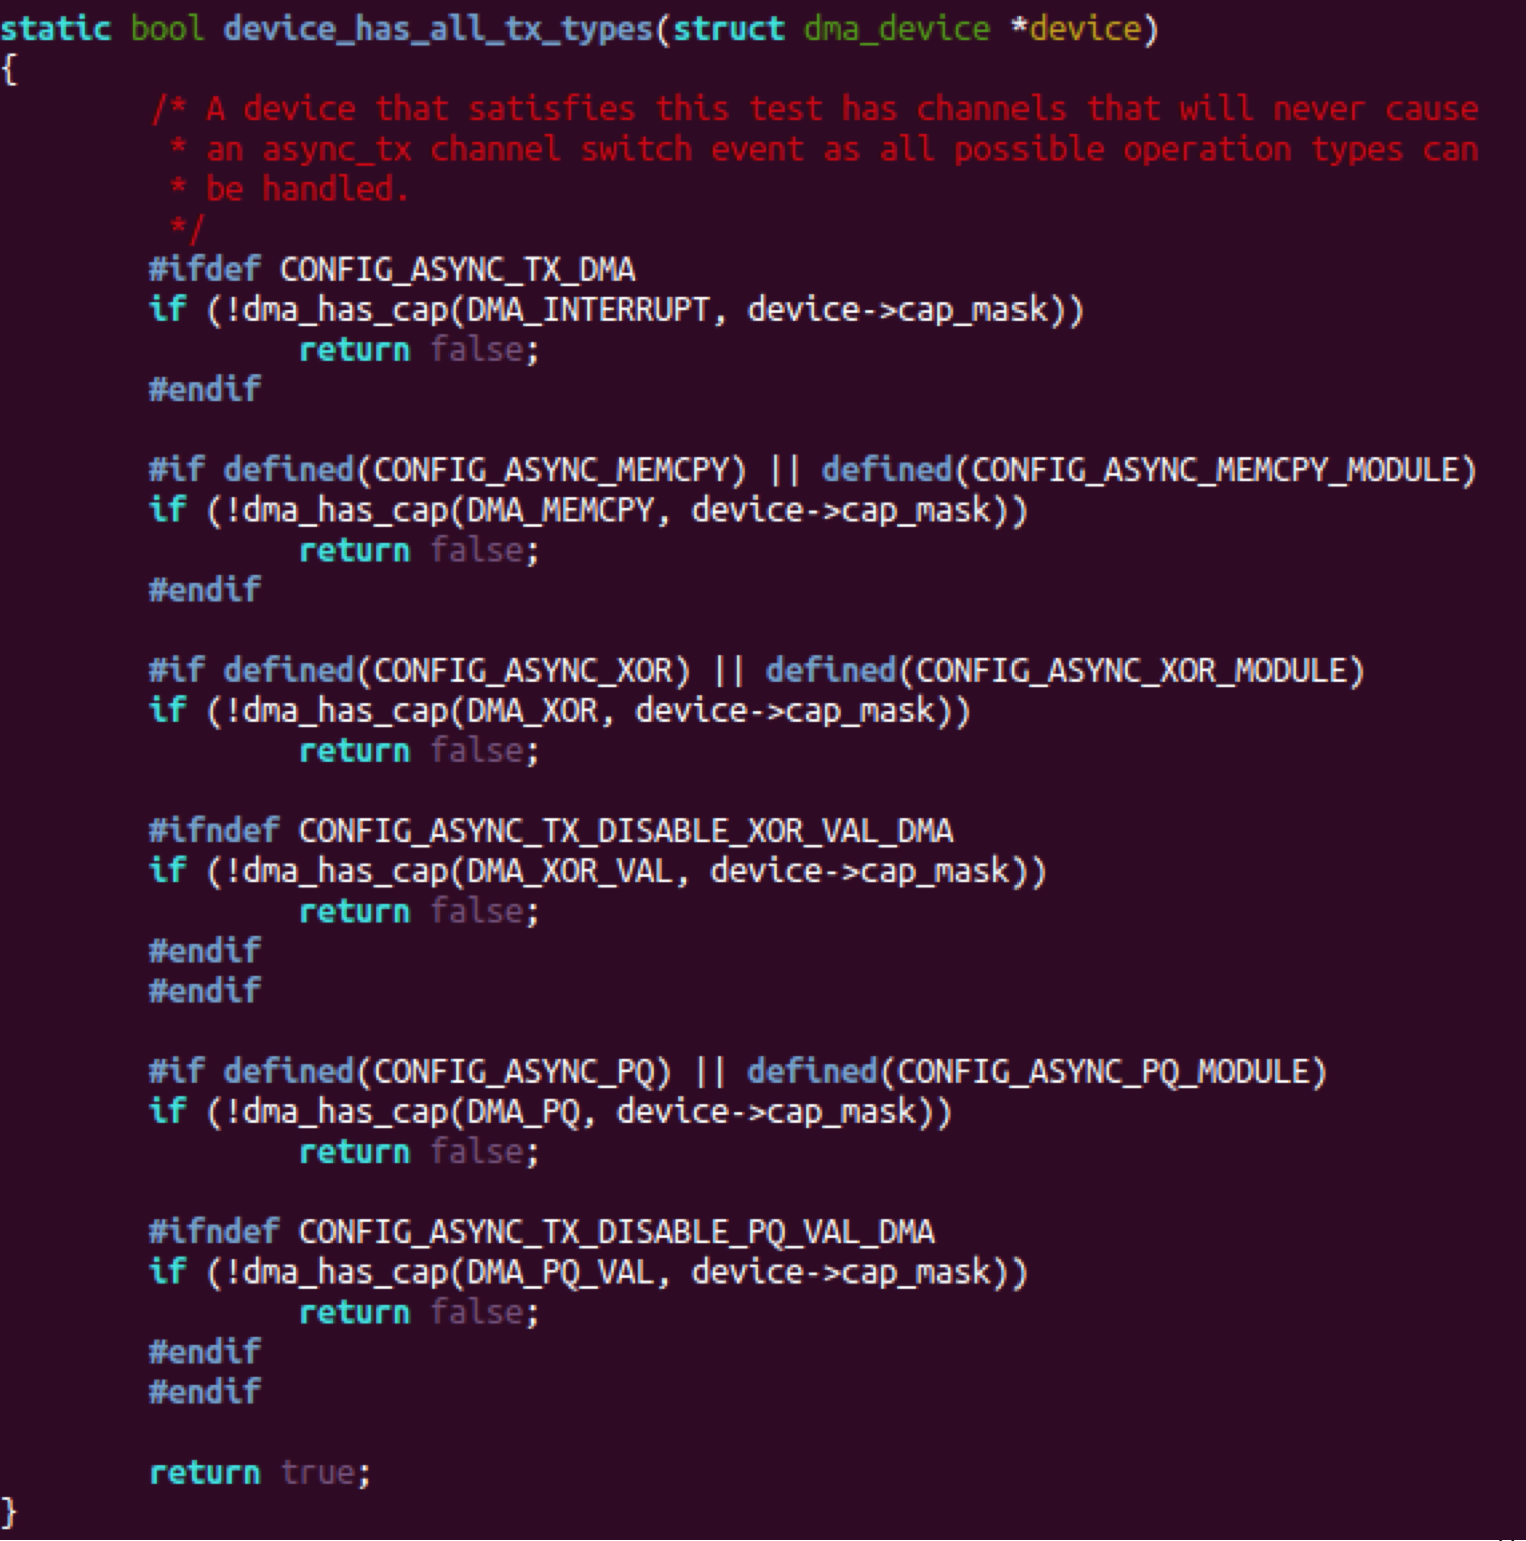
\includegraphics[width=\textwidth]{pic/dmaengine.eps}
  \caption{\acrshort{linux} Kernel /drivers/dma/dmaengine.c の一部}
  \label{dmaengine}
\end{figure}
\par
図\ref{dmaengine}の \verb|device_has_all_tx_types()| 関数では各設定値 \verb|CONFIG_***| に関する論理式が
複数の \verb|#if| または \verb|if| ブロックでネストされており、
全ての設定値を覚えていないとどこがコンパイル時に有効になるかを瞬時に把握することが困難である。
特に否定形の制御(\verb|#ifndef| や \verb|if(! ...)|)は人間にとって直感的に理解しづらい傾向があるため、
\verb|CONFIG_***_DISABLE_***| や \verb|#ifndef|、\verb|#if !definded|、\verb|if(! ...)|等が連結しているロジックは誤りの原因となることが多い。
このように、コンパイルスイッチは使い方によってはソフトウェアの挙動の理解を妨げ、デバッグやレビューの効率を低下させ、保守性を低下させ、結果として全体の品質低下を招く可能性がある。
例えばソフトウェアの挙動をコードと対応させて追いたい場合には、使われていない \verb|#ifdef| ブロックが一掃されたソースがあれば効率の良い解析が実施できると考えられる。
我々はこの問題に対して可読性の高いソースコードを得ることを目的に、有効な \verb|#ifdef| のみからなるソースコードを抽出する方法を調査した。
\acrshort{ot}のNicholas Mc Guireも同様な問題意識を持っており、2015年5月に
\href{https://gcc.gnu.org/ml/gcc-help/2015-05/msg00012.html}{\acrshort{gcc}コミュニティに対してコンパイラオプションに関する質問を行っている} \cite{fdirectives}。
\par
既存手法の調査を行った結果、
\href{http://stackoverflow.com/questions/7353640/strip-linux-kernel-sources-according-to-config}{\acrshort{overflow}上の記事「設定ファイルを元に\acrshort{linux} Kernel中の使われないコードを削除する方法」} \cite{overflow} で手掛かりを得た。
この記事で提案されている手順の概要は次のようなものであった。
\begin{enumerate}
  \item ビルドログを取得して全ての実行された \verb|gcc| コマンドを抽出する
  \item 各 \verb|gcc| コマンドからコンパイルオプション \verb|-c| 以降を消して \verb|-E -fdirectives-only| を加える \label{enum:stackstep2}
  \item 手順\ref{enum:stackstep2}で作成した \verb|gcc| コマンドを実行する
\end{enumerate}
\par
\verb|-E|は \verb|#include|、\verb|#define|、\verb|ifdef| 等に対するプリプロセスのみを行う \verb|gcc| オプションで、
\verb|-fdirectives-only|はプリプロセッサディレクティブへの処理のうちマクロの展開を抑制するオプションである。
\acrshort{overflow}の記事では上記ように \verb|gcc| オプションを駆使することで有効コードのみの抽出が可能であることが示されていたが、
この方法を\acrshort{linux} Kernelツリー全体に対して一括して適用する方法が未解決であった。
\par
我々はソースツリー全体でコンパイル対象のコードを抽出する方法を開発することを目標に、問題を次のように設定した。
\begin{itembox}[l]{\acrshort{codemini}の定義}
\acrshort{codemini}は以下の条件を満たすソースツリーを生成するソースコード変換処理とする。
\begin{itemize}
  \item コンパイル対象外の \verb|#ifdef| や \verb|#if| ブロックを含まない。
  \item \verb|#include| 行や \verb|#define| 行は元の形のまま保持される。
  \item ビルド対象のソースファイルのみを含む。
  \item 素のソースツリーでビルドした結果と同じバイナリを生成する。
\end{itemize}
\end{itembox}
\par
ここで"minimization"という言葉は"minimal configuration"とは異なる意味で用いている。
ソフトウェアに関して"minimization"と言う場合一般的には「最小構成の設定」を作ることを意味するが多いが、
ここでは上記の\acrshort{codemini}の定義に基づくソースコードの変換処理を意味するものとする。
\subsection{実現方針}
\acrshort{codemini}を実現するために、\acrshort{linux} Kernelを対象として以下の方針で実装の検討を行った。
\begin{enumerate}[label=(\roman*)]
  \item 既存 \verb|Makefile| の仕組み上で動作する構成とする \label{enum:makefile}
  \item プリプロセスコマンドを構築・実行する \label{enum:preprocess}
  \item 展開されたヘッダファイルの中身と余分な空白行を削除する \label{enum:postprocess}
\end{enumerate}
\subsubsection{\ref{enum:makefile} 既存Makefileの拡張}
\acrshort{linux} Kernelの \verb|Makefile| には、コンパイルと並行して何らかのソースコードチェックツールを実行するための
\verb|CHECK|変数が用意されている。
既定では\acrshort{sparse}が設定されており、これは \verb|make| コマンドで \verb|CHECK| 変数を上書きすることで
任意のチェックツールに置き換えることができる。
\verb|CHECK| 変数で指定されたチェックツールは \verb|make| コマンドで \verb|C| フラグを設定することにより実行される(図\ref{check})。
\begin{figure}[ht]
  \centering
  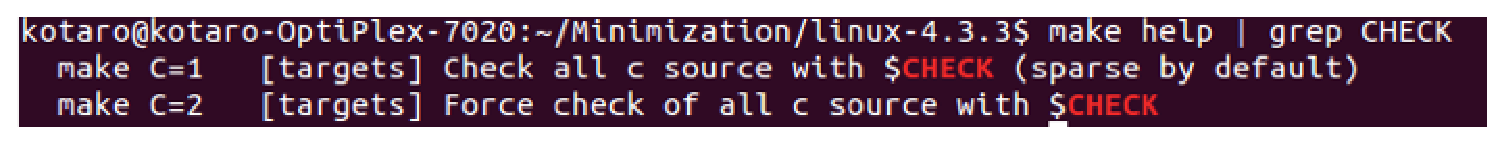
\includegraphics[width=\textwidth]{pic/check.eps}
  \caption{\acrshort{linux} KernelのMakefileで利用可能なソースコードチェック機能}
  \label{check}
\end{figure}
\par
\verb|CHECK| 変数で指定したチェックツールに対するオプションは、同じく \verb|make| コマンド中の \verb|CF| 変数で与えることができる(図\ref{cf})。
\begin{figure}[ht]
  \centering
  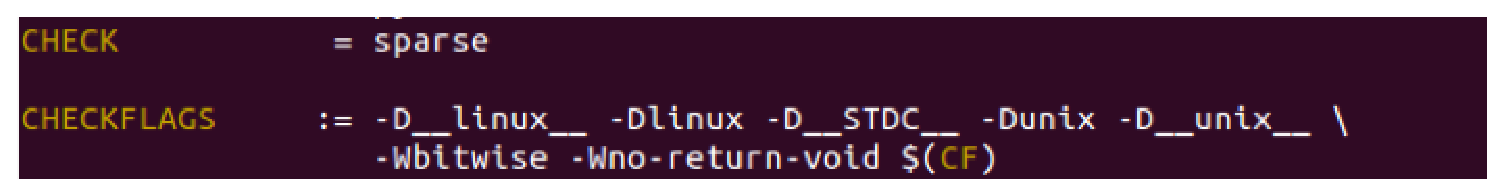
\includegraphics[width=\textwidth]{pic/cf.eps}
  \caption{\acrshort{linux} KernelのMakefile中で設定されているソースコードチェックツールとそのオプション}
  \label{cf}
\end{figure}
\par
\acrshort{codemini}の実装では、\acrshort{linux} Kernelの \verb|Makefile| に既に存在する図\ref{check}と図\ref{cf}の機能を利用して下記のようなコマンドで\acrshort{codemini}を実現する方針とした。
\begin{itembox}[l]{\acrshort{codemini}コマンド形式}
  \verb|make C=1 CHECK=minimize.py CF="-mindir ../minimized-tree"|
\end{itembox}
\par
\verb|minimize.py| は\acrshort{codemini}の\acrshort{py}スクリプトによる実装である。
\verb|CF| 変数で変換後のソースツリー生成場所を指定する。
これにより、通常のkernelビルドと同時に
各々のCソースファイルに対する\acrshort{codemini}が一括して実行される。
\verb|CHECK| 変数で指定したスクリプト \verb|minimize.py| には、各々のCソースファイルに対する \verb|gcc| コマンドと
同じオプション文字列が自動的に渡される。
そのため、\verb|CHECK| 変数を利用する方法は前述の\acrshort{overflow}の手順で必要だったビルドログの取得やgccコマンドの編集
といった中間処理が不要であり、全ての処理を1コマンドで完結できる利点がある。
\verb|minimize.py| スクリプト本体およびその詳しい使用手順は
\href{https://github.com/Hitachi-India-Pvt-Ltd-RD/minimization}{\acrshort{hub}のminimizationレポジトリで公開している} \cite{minimization}。
\subsubsection{\ref{enum:preprocess} プリプロセスコマンドの構築と実行}
以降は \verb|minimize.py| スクリプトの実装について処理の概要を記載する。
\par
\verb|minimize.py| は \verb|make| プロセスから呼ばれるとき、そのターゲットCファイルへの \verb|gcc| コマンドと同じオプション文字列を引数で受け取る。
\verb|minimize.py| は受け取ったオプション文字列の先頭に\verb|gcc -E -fdirectives-only | を追加した上で
その文字列をシステムコマンドとして実行する。
その結果、\verb|#ifdef| が消え、\verb|#include| が展開され、\verb|#define| がそのまま保存されたプリプロセス出力が得られる。
\subsubsection{\ref{enum:postprocess} 展開されたヘッダファイルの中身と余分な空白行の削除}
\verb|minimize.py| はプリプロセスの結果に対して \verb|#include| で展開されたヘッダファイルに該当する箇所を削除する。
\verb|gcc| のプリプロセス出力には以下のような形式で \verb|#include| の展開情報が残されており、これらは\textit{linemarkers}と呼ばれる。
プリプロセス出力からヘッダファイル展開箇所を特定するためには、\textit{linemarkers}を手掛かりとして用いる。
\begin{itemize}
  \item プリプロセス出力中の\textit{linemarkers}の例
  \begin{itemize}
    \item[] \verb|# 30 "/usr/include/sys/utsname.h" 2|
  \end{itemize}
\end{itemize}
\par
この\textit{linemarkers}の例は「この行以降のコードは \verb|/usr/include/sys/utsname.h| の30行目が展開されたもので、
かつ別の入れ子になった \verb|#include| の展開内容から返ってきた直後」であることを意味している。
\textit{linemarkers}の形式については以下のページが詳しい。 \\
 \href{https://gcc.gnu.org/onlinedocs/cpp/Preprocessor-Output.html}{Preprocessor Output - The C Preprocessor} \cite{linemarkers}
\par
\verb|minimize.py| は、\textit{linemarkers}を解析することで元のCファイルに存在しないヘッダファイルの展開内容を削除する。
その上で元のCファイルの内容と比較をして \verb|#include| 行の復元と、消えた \verb|#ifdef| ブロックに該当する空白行の削除を行う。
元のソースと最終的に得られるソースとの差分は無効な \verb|#ifdef| ブロックの削除のみであり、
\verb|#include| 行および \verb|#define| 行は元のまま保持される(図\ref{miniresult})。
\begin{figure}[ht]
  \centering
  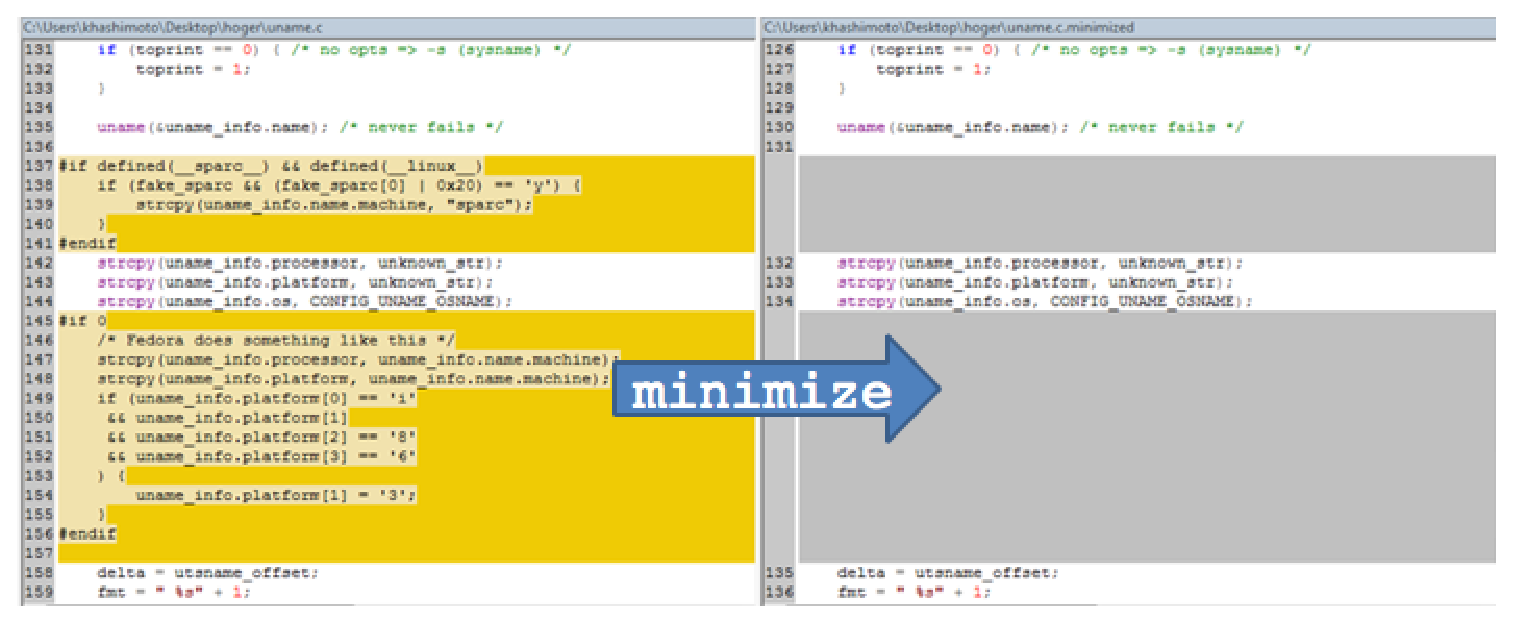
\includegraphics[width=\textwidth]{pic/miniresult.eps}
  \caption{\acrshort{codemini}の実行結果例}
  \label{miniresult}
\end{figure}
\par
\subsection{実行結果}
\verb|minimize.py| は当初\acrshort{linux} Kernelに対して適用することを想定して実装されたが、\verb|Makefile| 中の \verb|CHECK| 変数を利用する仕組みがそのまま
\acrshort{bb}にも適用できることが分かった。
\acrshort{linux} Kernelおよび\acrshort{bb}に対して \verb|minimize.py| を実行した結果削除されたソースコード量を表\ref{ministats}に示す。
ここでは実験対象として\acrshort{linux} Kernel 4.3.3と\acrshort{bb} 1.24.15を使用し、各々 \verb|allnoconfig| と \verb|defconfig| を適用したときの
\acrshort{codemini}結果を記載している。
実験はUbuntu 14.04 (x86\_64)で実施した。
\begin{table}[H]
  \caption{\acrshort{linux} Kernelと\acrshort{bb}への\acrshort{codemini}適用で削除されたコード量}
  \label{ministats}
  \centering
  \begin{tabular}{l|ll}
    設定 \textbackslash ターゲット & \acrshort{linux} Kernel 4.3.3 & \acrshort{bb} 1.24.15 \\
    \hline 
    \verb|defconfig| (x86) & 103144行(全体の5\%) & 20453行(全体の11\%)\\
    \verb|allnoconfig| & 64684行(全体の22\%) & 5945行(全体の34\%
%    \verb|defconfig| (x86) & \shortstack{103144行(全体の5\%) \\ $1804 / 2022$ファイルが処理対象} & \\
  \end{tabular}
\end{table}
\par
\acrshort{linux} Kernel、\acrshort{bb}ともに \verb|allnoconfig| 設定のときにコード削減割合が高い。
これは、無効化される機能が多くなるほど使用されない \verb|#ifdef| ブロックが増えることと対応している。
\par
\verb|minimize.py| 実行の結果生成されたソースツリーは素のソースツリーと同じ手順でビルドが可能であった。
ビルドの確認は、\acrshort{codemini}後のファイルとディレクトリをそのまま素のソースツリー上に上書きコピーして実施した。
これは\acrshort{codemini}生成物に \verb|Makefile| などのビルドに必要なスクリプト類が含まれないためである。
\par
\acrshort{codemini}は無効コードを削除するのみで、機能そのものには一切影響を与えてはいけない。
このことを確認するため、素のソースツリーのビルド生成物と\acrshort{codemini}で生成されたソースツリーのビルド生成物の比較を行うことを検討した。
各々ビルドの結果生成されたバイナリを \verb|objdump -d| コマンドで逆アセンブリしたところ、アセンブリコードの比較結果は表\ref{assemblycomp}のようになった。
\begin{table}[H]
  \caption{\acrshort{codemini}後のソースツリーによるビルド生成物と素のソースツリーによるビルド生成物とのアセンブリコード比較結果}
  \label{assemblycomp}
  \centering
  \begin{tabular}{l|ll}
    設定 \textbackslash ターゲットファイル & vmlinux.o & busybox(実行ファイル) \\
    \hline 
    \verb|defconfig| (x86) & 差分あり & 一致 \\
    \verb|allnoconfig| & 一致 & 一致
  \end{tabular}
\end{table}
\par
アセンブリコード( \verb|objdump -d| の出力)が一致するターゲットと設定の組み合わせに対してもバイナリファイルの直接比較結果は一致しない。
これはビルド生成物にビルドタイムスタンプ等の情報が埋め込まれていることが要因の一つである。
\verb|objdump -d| は実行ファイル中から実行部(executable section)のアセンブリコードを出力する。
表\ref{assemblycomp}において \verb|objdump -d| が一致することは、\verb|minimize.py| の処理内容が最終ビルド生成物の挙動に影響を与えないことを支持する。
しかし、\acrshort{linux} Kernelを\verb|defconfig| (x86)で\acrshort{codemini}適用した場合は、ビルド生成物のアセンブリコードと素のソースツリー由来のものとで差分があった。
この事象に対する調査、および \verb|minimize.py| がソフトウェアの機能そのものに一切影響を及ぼさないことの更なる検証方法検討は今後の課題である。
\par
\acrshort{linux} Kernelおよび\acrshort{bb}に対する\acrshort{codemini}実装は以下の\acrshort{hub}レポジトリで公開している(図\ref{minigithub})。\cite{minimization}
\begin{figure}[H]
%\begin{figure}[ht]
  \centering
  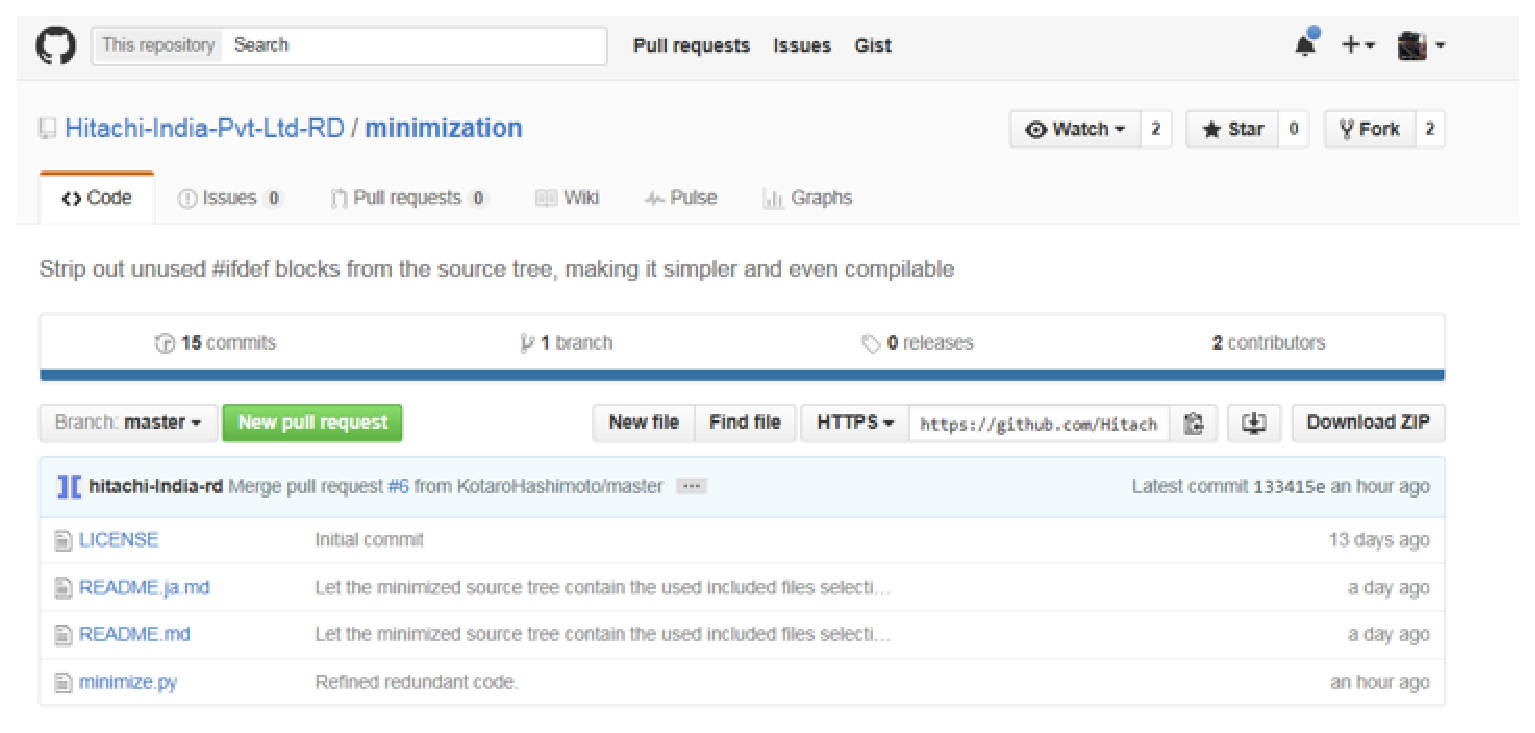
\includegraphics[width=\textwidth]{pic/minigithub.eps}
  \caption{\href{https://github.com/Hitachi-India-Pvt-Ltd-RD/minimization}{https://github.com/Hitachi-India-Pvt-Ltd-RD/minimization}}
  \label{minigithub}
\end{figure}
%\newline
\subsection{\acrshort{codemini}技法の利点と応用}
\acrshort{codemini}技法を適用することで、使用されないコードを削除することによるソースコードの可読性向上が期待される。
加えて、ソースコードのレビューや静的検証を行う際の検査対象範囲が限定される効果も考えられる。
本項では、可読性向上に関する評価と、検査対象範囲を限定することにより静的検証のパフォーマンスを向上させる応用例について記載する。
\subsubsection{変換後のソースコード複雑度評価}
\acrshort{codemini}適用によるソースコード可読性向上度合いを評価するため、ソースコードの複雑度を測定するツール
\href{https://www.gnu.org/software/complexity/manual/complexity.html}{\acrshort{comp}} \cite{comp}
を使用した。
\acrshort{comp}はCプログラムの複雑度を定量的に測定するために設計された\acrshort{gnu}ツールである。
コード複雑度の測定ツールとしては例えば\acrshort{mc}が知られている。
\acrshort{mc}は主に実行パス数に基づく情報からテストに必要な労力を数値化することを目的としているのに対して、
\acrshort{comp}はコードの長さや条件分岐の複雑さを評価することで、特に人間がコードを理解するための労力を数値化することを意図している。
\par
以下は、\acrshort{codemini}適用前の\acrshort{linux} Kernelソースツリー中のCソースファイルについて\acrshort{comp}で
複雑度を測定した結果である。
"Complexity Histogram"では、関数ごとに測定された複雑度スコアの分布($0 \sim 1999$)がコード行数の積算を度数として示されている。
複雑度スコアの平均値(Average line score)は23、中央値(50\%-ile score)は4、最大値(Highest score)は1846であった。
\begin{itembox}[l]{素の\acrshort{linux} Kernelソースツリーに対する\acrshort{comp}測定結果}
\small
\begin{verbatim}
$ find linux-4.4.1 -name "*.c" | xargs complexity -h
Complexity Histogram
Score-Range  Lin-Ct
    0-9      277794 ************************************************************
   10-19      49923 ***********
   20-29      17566 ****
   30-39       7189 **
   40-49       2148
   50-59       1961
   60-69        630
   70-79        563
   80-89        633
   90-99       1381

  100-199      5332 *
  200-299      2765 *
  300-399         0
  400-499         0
  500-599         0
  600-699         0
  700-799         0
  800-899         0
  900-999         0

 1000-1999     2345 *

Scored procedure ct:    18176
Non-comment line ct:   370230
Average line score:        23
25%-ile score:              2 (75% in higher score procs)
50%-ile score:              4 (half in higher score procs)
75%-ile score:              9 (25% in higher score procs)
Highest score:           1846 (setgamma() in linux-4.4.1/drivers/media/usb/gspca/topro.c)
\end{verbatim}
\end{itembox}
\par
次に、\verb|allnoconfig| 設定で\acrshort{codemini}適用した\acrshort{linux} Kernelソースツリーに対して複雑度を測定した結果を示す。
複雑度スコアの平均値(Average line score)は5、中央値(50\%-ile score)は2、最大値(Highest score)は158であった。
なお、\acrshort{codemini}適用前の測定結果で複雑度スコアが最大であった関数 \verb|setgamma() (linux-4.4.1/drivers/media/usb/gspca/topro.c)|
は\acrshort{codemini}適用後のソースツリーに含まれていなかった。
\begin{itembox}[l]{allnoconfig 設定の\acrshort{linux} Kernelソースツリーに対する\acrshort{comp}測定結果}
\small
\begin{verbatim}
$ find minimized-tree -name "*.c" | xargs complexity -h
Complexity Histogram
Score-Range  Lin-Ct
    0-9       85190 ************************************************************
   10-19       7640 *****
   20-29       1004 *
   30-39        944 *
   40-49        102
   50-59        109
   60-69         96
   70-79          0
   80-89          0
   90-99          0

  100-199       396

Scored procedure ct:     7870
Non-comment line ct:    95481
Average line score:         5
25%-ile score:              1 (75% in higher score procs)
50%-ile score:              2 (half in higher score procs)
75%-ile score:              5 (25% in higher score procs)
Highest score:            158 (zlib_inflate() in minikern/lib/zlib_inflate/inflate.c)
Unscored procedures:        4
\end{verbatim}
\end{itembox}
\par
続いて、\verb|defconfig| (x86)設定で\acrshort{codemini}適用した\acrshort{linux} Kernelソースツリーに対して複雑度を測定した結果を示す。
複雑度スコアの平均値(Average line score)は7、中央値(50\%-ile score)は3、最大値(Highest score)は194であった。
\begin{itembox}[l]{defconfig(x86)設定の\acrshort{linux} Kernelソースツリーに対する\acrshort{comp}測定結果}
\small
\begin{verbatim}
$ find minimized-tree -name "*.c" | xargs complexity -h
Complexity Histogram
Score-Range  Lin-Ct
    0-9      675258 ************************************************************
   10-19      86562 ********
   20-29      27818 **
   30-39      12037 *
   40-49       5734 *
   50-59       2583
   60-69       3124
   70-79       3047
   80-89        281
   90-99       1051

  100-199      2135

Scored procedure ct:    50155
Non-comment line ct:   819630
Average line score:         7
25%-ile score:              2 (75% in higher score procs)
50%-ile score:              3 (half in higher score procs)
75%-ile score:              7 (25% in higher score procs)
Highest score:            194 (inflate_fast() in minikern/lib/zlib_inflate/inffast.c)
Unscored procedures:        9
\end{verbatim}
\end{itembox}
\par
以上を総合すると、複雑度スコアの平均値、中央値、最大値はいずれも \verb|allnoconfig| $<$ \verb|defconfig| $<$ (\acrshort{codemini}非適用) の関係となり、
\acrshort{codemini}によって削除されたコード量の大小と対応する結果が得られた(表\ref{kcomp})。
\begin{table}[H]
  \caption{\acrshort{linux} Kernelソースツリーの\acrshort{codemini}適用前後に対する\acrshort{comp}スコア測定結果}
  \label{kcomp}
  \centering
  \begin{tabular}{l|lll}
    \normalsize{スコア種類 \textbackslash 設定条件} & \verb|allnoconfig| & \verb|defconfig| (x86) & \acrshort{codemini}非適用 \\
    \hline 
    平均値(Average line score) & 5 & 7 & 23 \\
       (25\%-ile score) & 1 & 2 & 2 \\
    中央値(50\%-ile score) & 2 & 3 & 4 \\
       (75\%-ile score) & 5 & 7 & 9 \\
    最大値(Highest score) & 158 & 194 & 1846
  \end{tabular}
\end{table}
\par
同様の複雑度測定評価を\acrshort{bb}に対して行った結果を表\ref{bcomp}に示す。
\acrshort{bb}での測定結果においても\acrshort{linux} Kernelと同様に概ね \verb|allnoconfig| $<$ \verb|defconfig| $<$ (\acrshort{codemini}非適用) の関係が得られた。
\begin{table}[H]
  \caption{\acrshort{bb}ソースツリーの\acrshort{codemini}適用前後に対する\acrshort{comp}スコア測定結果}
  \label{bcomp}
  \centering
  \begin{tabular}{l|lll}
    \normalsize{スコア種類 \textbackslash 設定条件} & \verb|allnoconfig| & \verb|defconfig| (x86) & \acrshort{codemini}非適用 \\
    \hline 
    平均値(Average line score) & 19 & 21 & 22 \\
       (25\%-ile score) & 2 & 3 & 3 \\
    中央値(50\%-ile score) & 5 & 9 & 9 \\
       (75\%-ile score) & 21 & 24 & 25 \\
    最大値(Highest score) & 283 & 283 & 283
  \end{tabular}
\end{table}
\par
以上から、\acrshort{codemini}で無効コードを削除した結果では
\acrshort{comp}ツールによる客観的な指標においてソースコードの可読性が向上することが示された。
\subsubsection{検査対象範囲の最小化}
\label{minigraph}
本項では、\acrshort{codemini}がソースコードの検査対象範囲を限定する効果に着目し、
その性質を応用することで静的検証におけるパフォーマンスを向上させることができる例を示す。
\par
テストカバレッジ測定の原理を考えたとき、一般にテストカバレッジは
テスト実施した行数($LOC_{exercised}$)の総コード行数($LOC_{total}$)に対する比で表される(式(\ref{usocov}))。
\begin{equation}
  TestCoverage = \frac{LOC_{exercised}}{LOC_{total}}
\label{usocov}
\end{equation}
\par
ここで、コンパイル対象とならない無効な \verb|#ifdef| コードブロックがソースコードに含まれる場合は
無効なコードブロック行数$LOC_{unused}$を$LOC_{total}$から引くことでより正確なカバレッジが測定できる(式(\ref{minicov}))。
\begin{equation}
  TestCoverage = \frac{LOC_{exercised}}{LOC_{total} - LOC_{unused}}
\label{minicov}
\end{equation}
\par
式(\ref{minicov})は、使用されないコードを多く特定するほど計算上テストカバレッジが向上する(より正確なカバレッジ評価となる)ことを意味する。
使用されないコードが特定されない限り、$LOC_{exercised}$を増やすためにどれだけテストに労力を費やしたとしても
達成できるカバレッジは100\%未満($1 - \frac{LOC_{unused}}{LOC_{total}}$)で制限される(図\ref{coveragesagi})。
ここで\acrshort{codemini}適用により$LOC_{unused}$を明らかにすることができれば、
達成し得るテストカバレッジをその分向上させることができる。
このように、\acrshort{codemini}は検査範囲を最小化する効果がある。
この技法を"minimization"と呼ぶことはこの意味での「最小化」の効果が得られることに由来する。
\begin{figure}[ht]
  \centering
  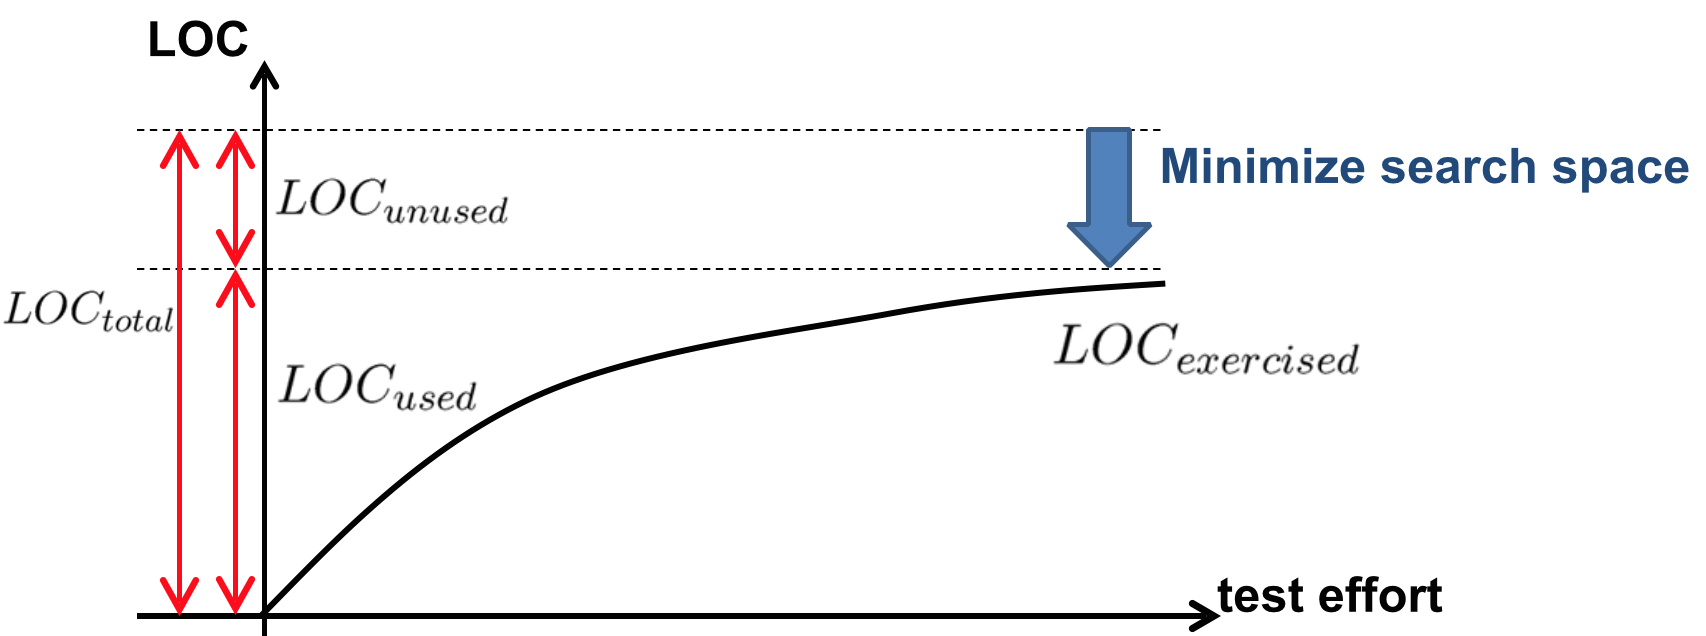
\includegraphics[width=\textwidth]{pic/coveragesagi.eps}
  \caption{\acrshort{codemini}適用により正確なテストカバレッジ測定が可能となる}
  \label{coveragesagi}
\end{figure}
%\paragraph{関数コールグラフを枝刈りする応用例}\mbox{}\\
\subsubsection{関数コールグラフを枝刈りする応用例}
\acrshort{codemini}で予めソースコードを最小化することで関数コールグラフの解析が簡単になる例を示す。
\ref{callgraph}項で述べたように、関数コールグラフはトレーサと組合わせてパスカバレッジを測定する目的で使用できる。
関数コールグラフ導出により実行され得る全関数呼び出しパスを特定することは、式(\ref{minicov})において分母($LOC_{total} - LOC_{unused}$)に相当にする箇所を測定することに対応する。
\par
ここでは\acrshort{cflow}を使用して\acrshort{bb}の \verb|init_main() (init/init.c)| に対する関数コールグラフを生成する。
グラフ画像生成は次のコマンドで実施した。
\begin{itemize}
  \item \acrshort{cflow}で\acrshort{bb}から \verb|init_main()| の関数コールグラフを生成する手順
  \begin{itemize}
    \item[] \verb!$ cd busybox-1.24.1!
    \item[] \verb!$ cflow -d 5 -b init/init.c | tree2dotx | dot -Tsvg -o init.svg!
  \end{itemize}
\end{itemize}
\par
\acrshort{codemini}適用前の関数コールグラフを図\ref{orggraph}に示す。
このグラフは \verb|#ifdef| ブロックで無効化される関数も含まれているため複雑で非常に見通しが悪い。
\acrshort{codemini}適用前グラフのノード数は94、エッジ数は140であった。
図\ref{minigraph}は\acrshort{codemini}適用後の関数コールグラフである。
こちらのグラフはコンパイル対象である関数のみが含まれるため複雑さが改善している。
\acrshort{codemini}適用後のグラフのノード数は85、エッジ数は123であった。
\begin{figure}[ht]
 \begin{minipage}{0.53\hsize}
  \begin{center}
   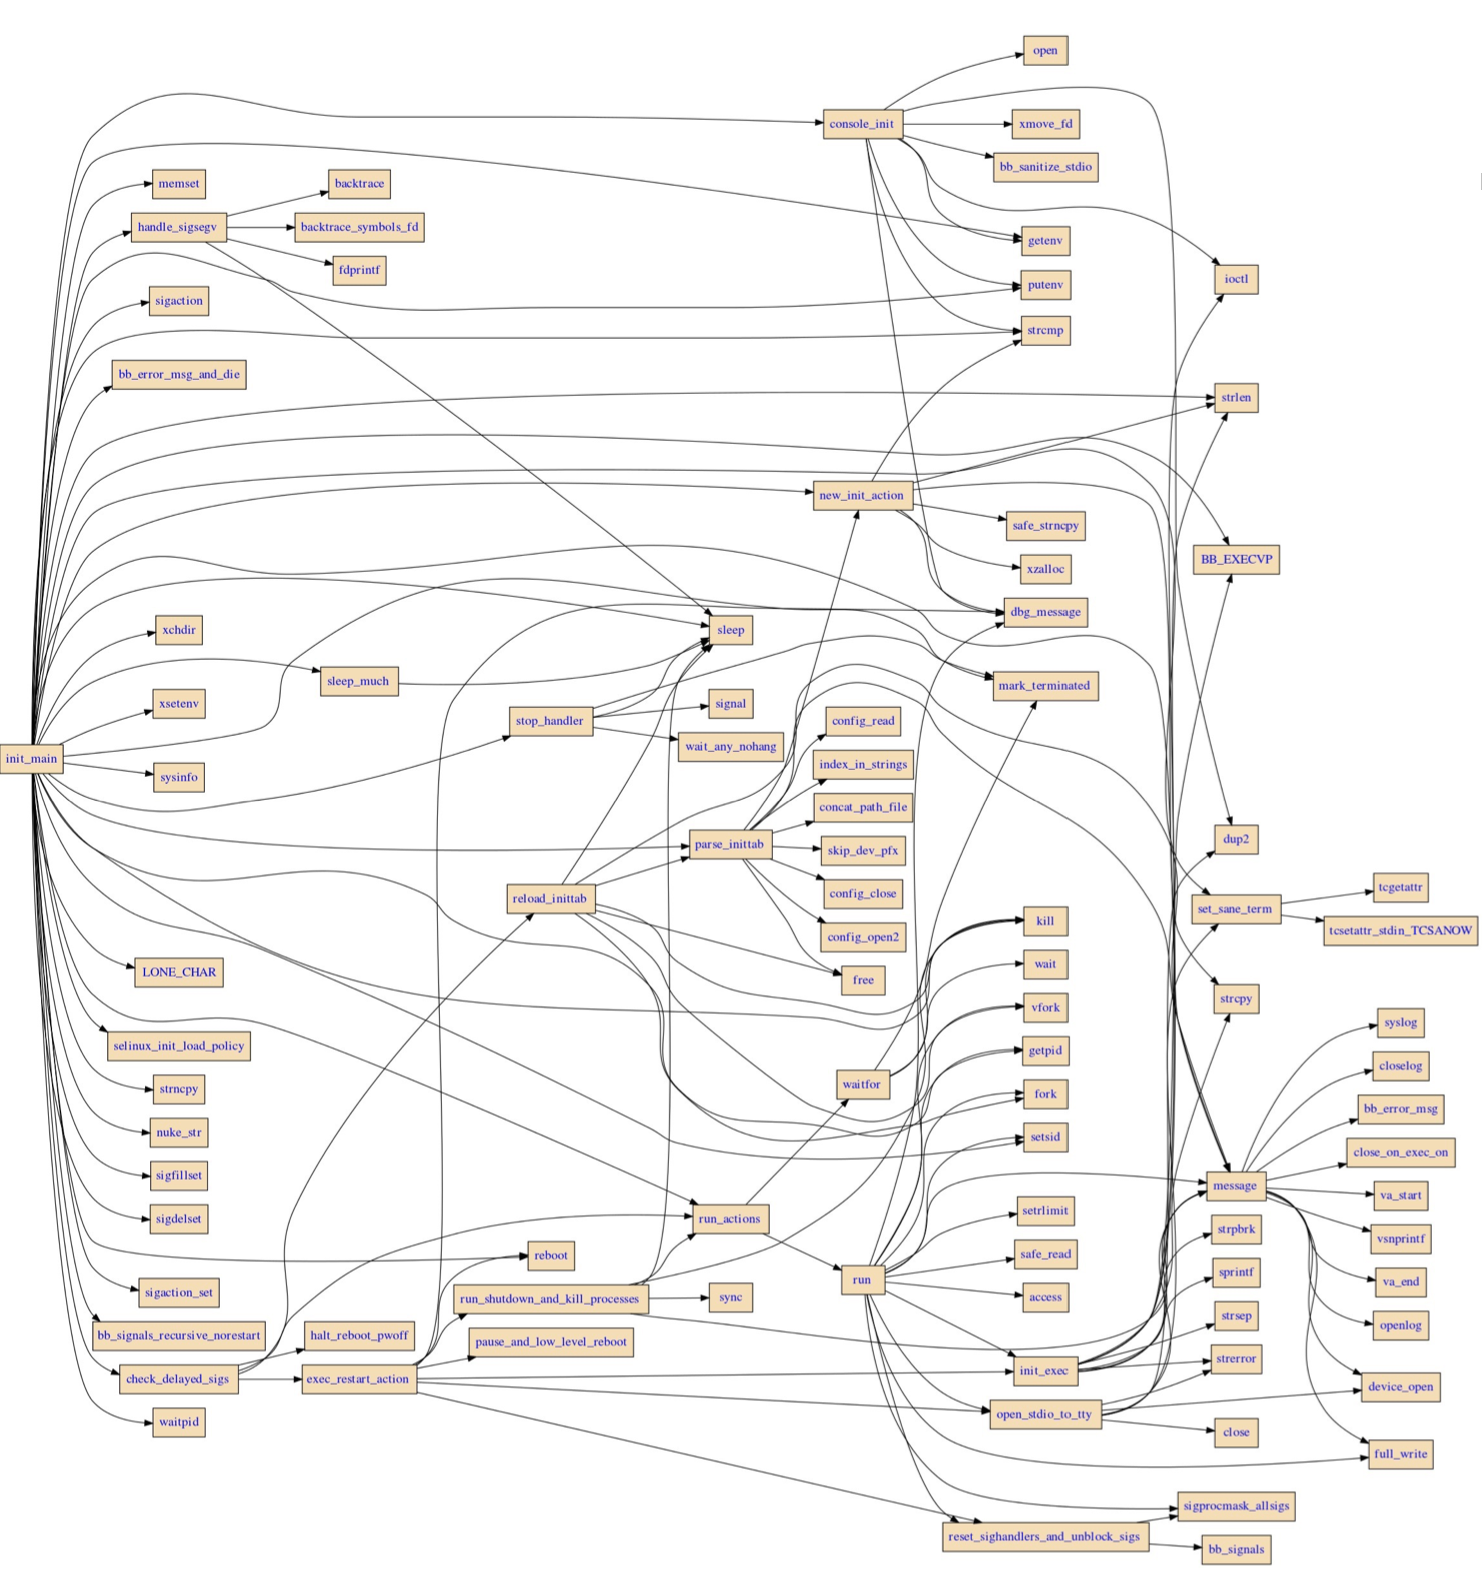
\includegraphics[width=\textwidth]{pic/orggraph.eps}
  \end{center}
  \caption{適用前(94ノード、140エッジ)}
  \label{orggraph}
 \end{minipage}
 \begin{minipage}{0.47\hsize}
  \begin{center}
   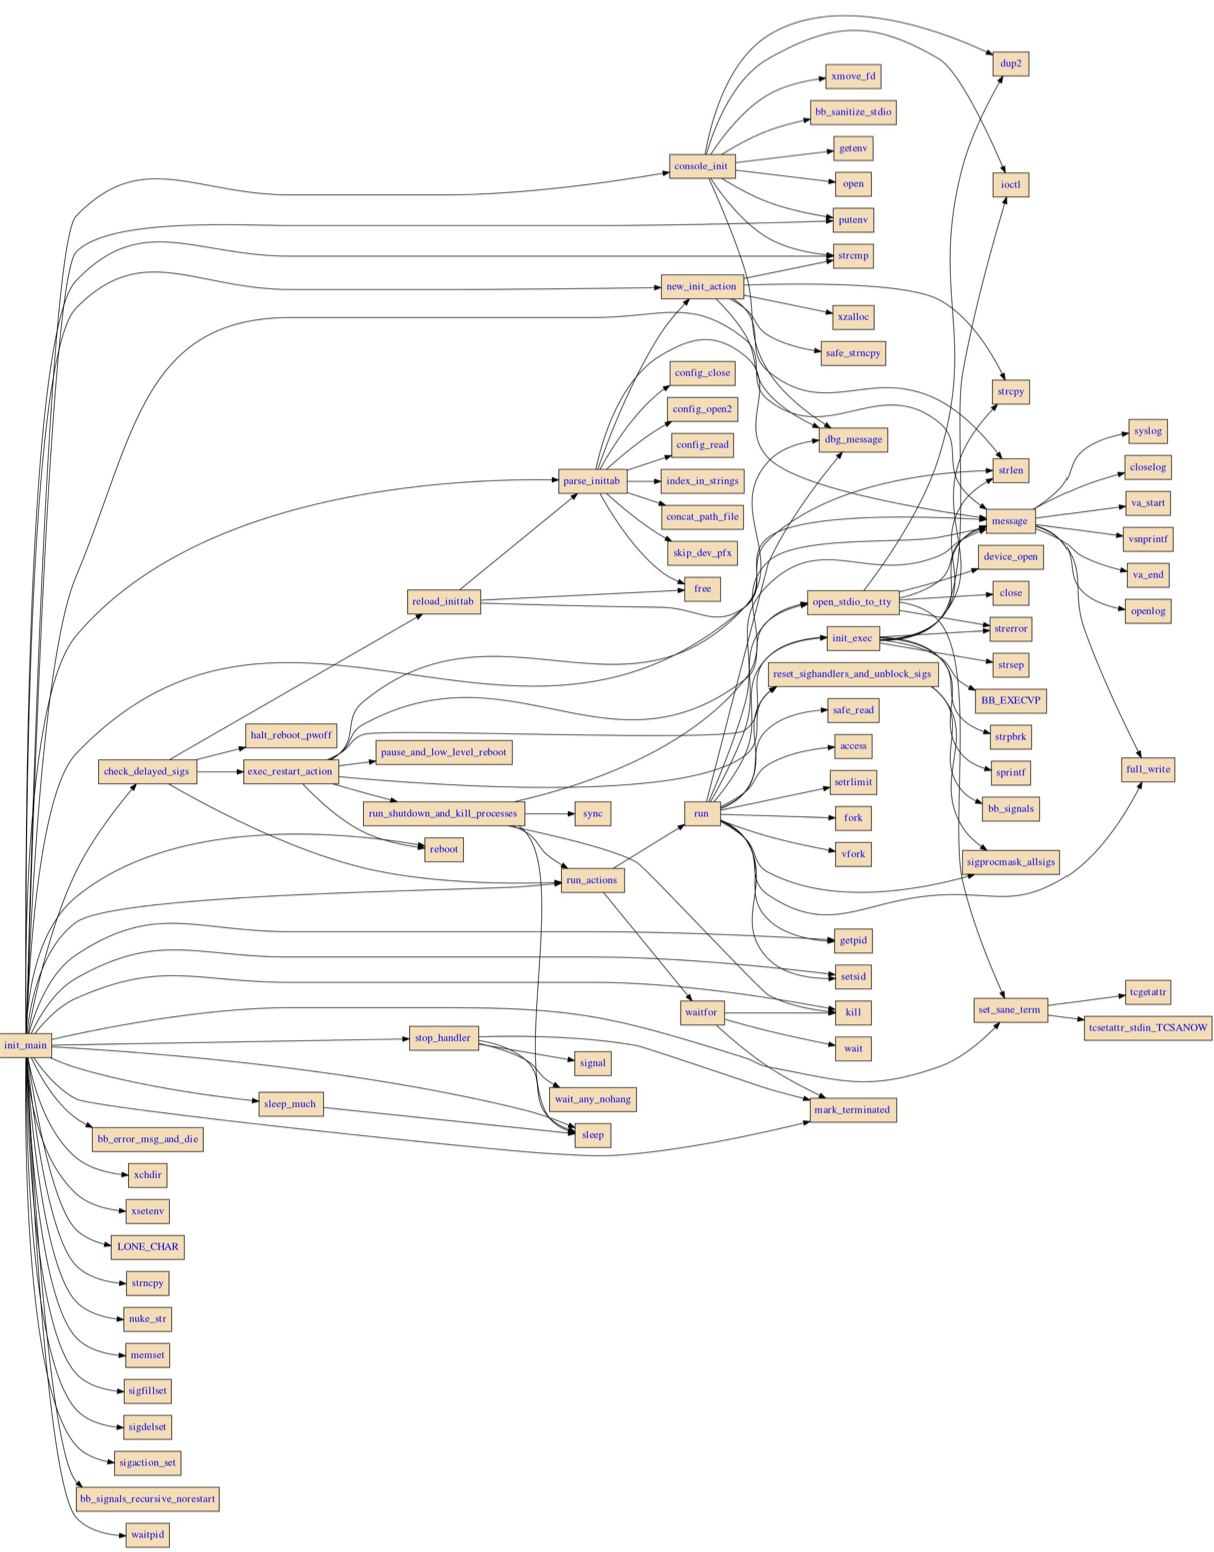
\includegraphics[width=\textwidth]{pic/minigraph.eps}
  \end{center}
  \caption{適用後(85ノード、123エッジ)}
  \label{minigraph}
 \end{minipage}
 \caption{\acrshort{codemini}適用前後の関数コールグラフサイズ比較}
\end{figure}
\par
以上の結果から、関数コールグラフ解析において事前に\acrshort{codemini}を実施することで
グラフのサイズを最小化することができ、解析の効率向上やカバレッジ向上等の効果を期待できることが分かる。
ちなみに \verb|cflow| コマンド自体にもプリプロセスオプションが備わっているため、\acrshort{codemini}を使用しなくとも
コンパイル対象外の関数をグラフに含めないことは可能である。
ただし、\verb|cflow| コマンドでプリプロセスを行う場合は \verb|gcc| コンパイルオプション文字列をビルドログから取得して
\verb|cflow| の \verb|--cpp| オプションで渡す作業を各Cファイルについて行わなければならず、手間がかかる上に誤りが発生しやすい。
それに対して \verb|minimize.py| は1コマンドで一括して全てのCファイルに対するプリプロセスを行うことができる利点がある。
\par
\acrshort{cflow}に限らず、\acrshort{cocci}や\acrshort{cpa}等の各種検証ツールもそれぞれプリプロセスオプションが備わっていることが多い。
ただし、各検証ツールはプリプロセス自体が主目的ではないためそれらのプリプロセス処理は \verb|gcc| のものと比べて完全でないことが多く、
中には独自のプリプロセス挙動を示すものもある。
\verb|minimize.py| は変換後のソースツリーも元と同じ手順でビルド可能であることを保証するものであり、
これは\acrshort{codemini}技法が特定の検証ツールに依存せず一般に様々な検証技法の前処理として応用できることを示唆する。
\subsubsection{部分ソースツリーの抽出}
\verb|minimize.py| は \verb|Makefile| がサポートするサブターゲットに対しても作用する。
\verb|minimize.py| を実行する \verb|make|コマンドでサブターゲットを指定した場合、
そのサブターゲットが依存するソースファイルのみを含む部分ツリーが抽出される。
抽出された部分ツリー中のCソースファイルは\acrshort{codemini}適用後の状態となる。
以下は、\acrshort{bb}の \verb|init| サブターゲットから依存されるソースファイルを、
コンパイル対象のコードブロックのみを含む形で部分的に抽出するコマンド例である。
\begin{itemize}
  \item \acrshort{bb}の \verb|init| サブターゲットで使われるソースファイルとコードのみを抽出するコマンド例
  \begin{itemize}
    \item[] \verb!$ cd busybox-1.24.1!
    \item[] \verb!$ make init C=2 CHECK=minimize.py CF="-mindir ../min-init"!
  \end{itemize}
\end{itemize}
\par
上記コマンドの実行結果抽出された部分ソースツリーは図\ref{subtarget}のようになる。
\begin{figure}[ht]
  \centering
  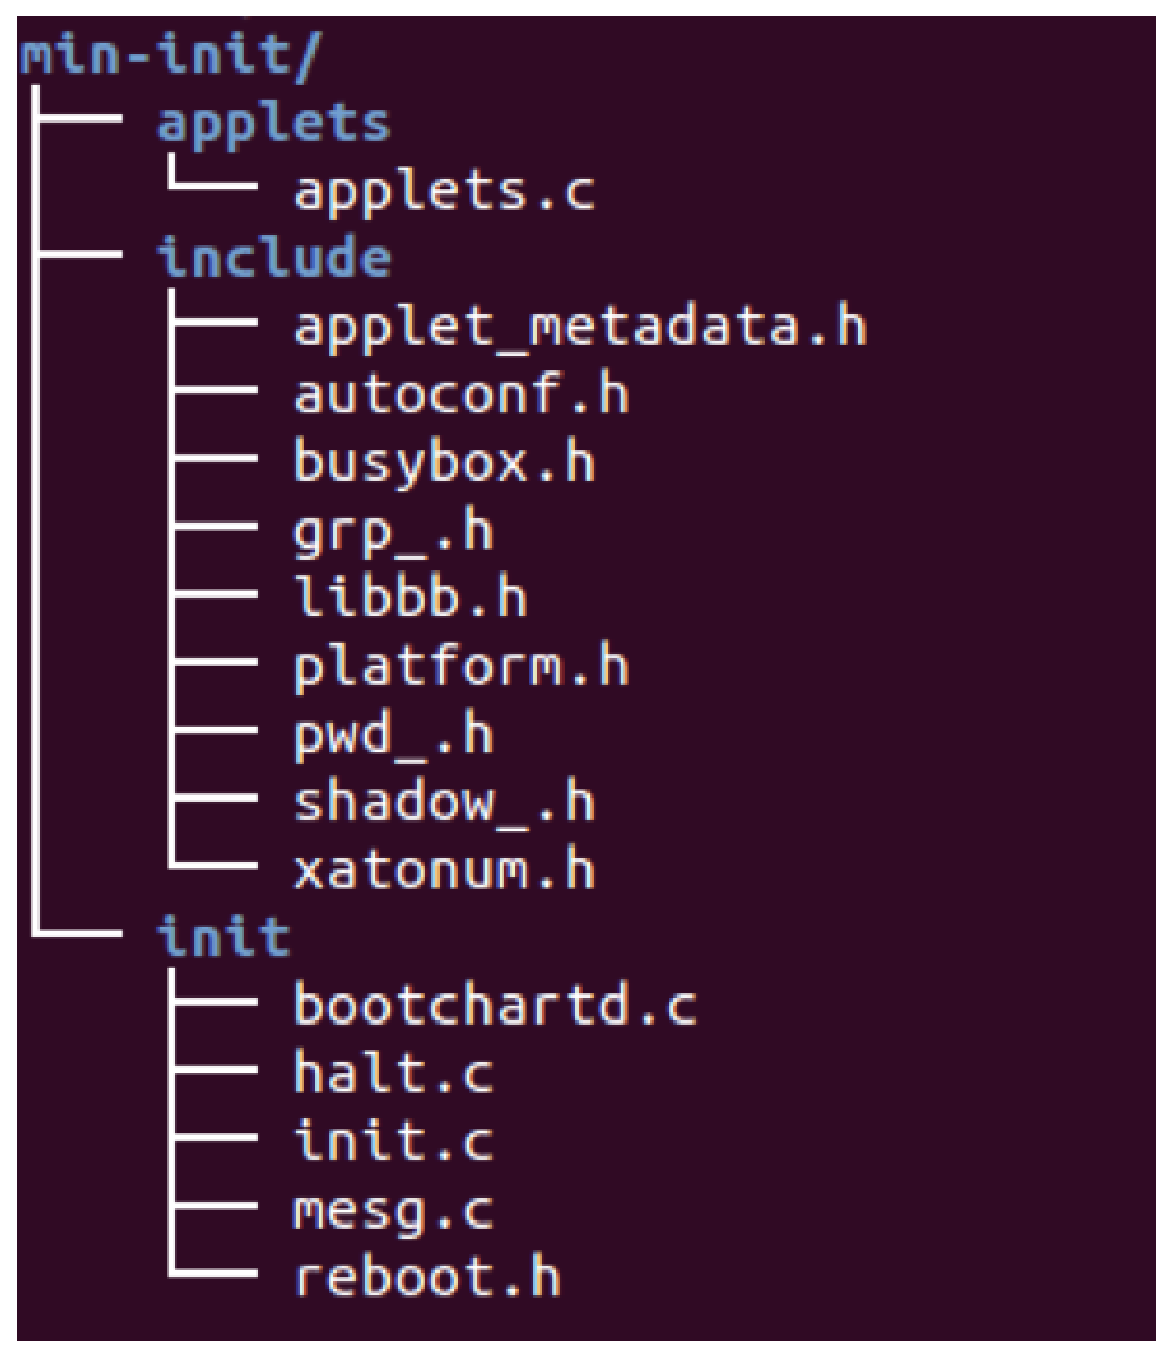
\includegraphics[width=0.4\textwidth]{pic/subtarget.eps}
  \caption{\acrshort{bb}のinitサブターゲット対象に\acrshort{codemini}適用して得られた部分ツリー}
  \label{subtarget}
\end{figure}
\par
指定したサブターゲットからどのファイルが実際にコンパイル対象として使われているかが明らかになることで、
例えばコードレビューの効率が向上する効果が期待される。
\subsection{まとめと今後の課題}
\acrshort{codemini}技法はソースコードの可読性を向上させる効果がある。
この性質はコードレビューやデバッグ効率向上のために利用できる。
また、\acrshort{codemini}技法は検査対象範囲を限定する効果がある。
これは図\ref{100} (\acrshort{iec61508}-3 Table B.2 - Dynamic analysis and testing)において
各種カバレッジ100\%を達成するために有力な手段となる。
または、テストを実施しない箇所がコンパイル対象外であることに示すエビデンスとして\acrshort{codemini}の結果を利用することも考えられる。
使用されないコードを特定し検査対象から除外することは、検証ツールが生成する\acrshort{fp}絶対量を抑制する結果にもつながる。
さらに、全体のコード量が削減されることで静的検証に要する時間と計算資源コストを節約できる。
Nicholas Mc Guire(\acrshort{ot})の実験によると、3時間要していた\acrshort{cocci}実行が\acrshort{codemini}適用後のソースツリーでは15分程度に短縮されたという。
\par
現状 \verb|minimize.py| がサポートするターゲットは\acrshort{linux} Kernelと\acrshort{bb}で、変換後ソースツリーのビルドを確認した設定は \verb|allnoconfig|、\verb|defconfig| (x86)、および \verb|omap2plus_defconfig|(ARMターゲットへのクロスビルド)である。
今後はさらに適用できるターゲットと設定を拡充していく予定である。
また\acrshort{codemini}適用後のソースツリーが素のソースツリーと機能的に等価であることの検証が未解決課題である。
\par
\acrshort{codemini}は一般に検証ツール・手法のパフォーマンスを増強させる技法であるため、組み合わせによって様々な使い方の可能性がある。
今後多数の\acrshort{codemini}技法の応用方法を考案し、\acrshort{sil2linuxmp}コミュニティに提案を行っていく方針である。

\chapter{今後の業務への貢献・活用}
\acrshort{sil2linuxmp}プロジェクトは2017年11月までに完結することが目標とされている。
プロジェクト2年目となる2016年度では、日立はこれまでと同様に\acrshort{sil2linuxmp}コミュニティへの働きかけを継続するとともに、
\acrshort{sil2linuxmp}プロジェクトで得た知見を社内の製品開発に還元していく活動を行う。
2016年度に実施すべき課題として以下の3つを設定する。
\begin{itemize}
  \item \acrshort{oss}・\acrshort{linux}システムの機能安全対応パイロット開発実施
  \item 機能安全対応\acrshort{linux}ディストリビューションの構築と提案
  \item \acrshort{sil2linuxmp}コミュニティへの継続的なコントリビューション
\end{itemize}
\section{\acrshort{oss}・\acrshort{linux}システムの機能安全対応パイロット開発実施}
\acrshort{sil2linuxmp}プロジェクトは特定のシステムに対して機能安全認証を与えることを目指すのではなく、
一般に\acrshort{oss}・\acrshort{linux}を使ったシステムで機能安全認証を達成するためのプロセスおよび方法論を確立することを意図している。
そのため、開発されたプロセスと方法論が現実の製品に即して適用できることの事例を残すことが、
将来\acrshort{sil2linuxmp}の成果によって\acrshort{oss}・\acrshort{linux}が\acrshort{sc}なシステムで使われるようになるために重要である。
特に、現在\acrshort{sil2linuxmp}で開発されている\acrshort{cr}
(\acrshort{iec61508}文書をRoute$3_S$: assessment of non-compliant developmentに基づいて
\acrshort{oss}・\acrshort{linux}システムに適用できるよう解釈し具体的な手段を対応させたもの)
の詳細や実現方法が不完全であると\acrshort{tuv}から指摘されている。
この問題の一因として、\acrshort{sil2linuxmp}プロジェクトにおいてターゲットとなるユースケースとシステム構成が定まっていないために、
具体的に何に対してどのようにプロセス・方法論を適用するのかがコミュニティ内で明確に共有されていないことが挙げられる。
\par
日立はグループ内で開発されている\acrshort{linux}ベースの\gls{adas}に機能安全認証を与えることを目標に
\acrshort{sil2linuxmp}で開発されたプロセスと方法論の適用を試みることで、
\acrshort{cr}の具体化と\acrshort{oss}・\acrshort{linux}の\acrshort{sil2}対応事例確立を目指す。
この活動はソースコード自体の開発よりも、開発プロセスのトレーサビリティと開発体制の健全性を確保すること、
および定められたプロセスが適切に実施されていることのエビデンスを体系的に蓄積することが中心となる。
特に、使用するソフトウェアの選定、アーキテクチャ設計、リスク分析など特定の個人の評価に依存しがちな
様々な判断事項について、その判断に至るまでの議論の経過と判断基準を全て記録することが必要となる。
これらの記録は第三者認証機関のレビューを受ける場において、自ら構築したシステムが正しく設計されていることを証明するための材料となる。
日立ではこのことを「基本と正道」と言う。
同様の概念が\href{http://www.slideshare.net/chika_nakazawa/ss-27726686}{サイボウズでは「公明正大」と言われている}。 \cite{cybozu}
\par
具体的には、\acrshort{sil2linuxmp}プロジェクトで定期的に行われている\gls{hazop}セッションを利用して日立\acrshort{adas}システムのハザード分析を行う。
\acrshort{hazop}はシステムの潜在危険因子を定量的かつ網羅的に抽出・評価するプロセスで、予め定められた役割と手法によるチームワークで進行する。
\acrshort{sil2linuxmp}コミュニティは\acrshort{irc}とwebベースのツールを活用して\acrshort{hazop}をオンラインで行う仕組みを構築しており、
これによって遠隔メンバの参加や議論内容の確実な保存と事後参照が可能となっている。
また\acrshort{db4sil2}(\ref{db4sil2sec}項)を利用して検証結果のエビデンスを保存することや、
ソフトウェア部品とツールの選定評価基準を定めた\acrshort{sil2linuxmp}ドキュメント\gls{atc}に基づいた評価、
および\acrshort{ogsn}を利用してその評価過程を可視化する活動を行う。
\section{機能安全対応\acrshort{linux}ディストリビューションの構築と提案}
\acrshort{sil2linuxmp}と関連して、日立製品の共通ソフトウェア基盤として使用されることを目的とした独自の\acrshort{linux}ディストリビューション開発が進行している。
これは特に\acrshort{sc}な産業・インフラ分野で10年単位の長期間にわたって稼動するシステムを意図したものであり、
将来的に\acrshort{sil2linuxmp}の成果を取り込むことで機能安全案件にも対応できるサービスを実現することが計画されている。
\par
\acrshort{linux}ディストリビューションが多くのユーザに使用してもらえるようになるためには、タイムリーなメンテナンスサポートを継続的に提供することが必須である。
一般的に使用されているディストリビューションは全てパッケージ管理システムを持っており、ユーザはこれによって必要なバグ修正やセキュリティ更新を簡単な手順で適用することができる。
このようなメンテナンスサポートがないと、ユーザが全ての\acrshort{oss}アップストリームを監視して適用すべき変更を自分自身で判断した上で適用評価まで行わなければならないことになり、
\acrshort{linux}システム上でのアプリケーション開発にとって非現実的な量の負担となる。
%\par
我々が手厚いメンテナンスサービスを利用できるのはディストリビュータに所属するその分野のエキスパートの貢献に負うところが大きく、それはある意味属人的なプロセスでもある。
\acrshort{iec61508}-3 7.8 Software modification の項目に「ソフトウェアの改変プロセスが適切に定義され透明性を持って運用されること」という旨の内容が語られている通り、
機能安全対応のディストリビューション開発においてはアップストリームの監視とバグ修正・セキュリティ更新の適用評価プロセスのトレーサビリティが確保されることが求められる。
独自に機能安全対応\acrshort{linux}ディストリビューションを構築するとなると、数ある\acrshort{oss}プロジェクトを属人的でないプロセスで監視するためには何らかの自動化対策が不可欠となる。
\par
\acrshort{sil2linuxmp}プロジェクトでは\pageref{scale}ページで述べたように検証プロセスを自動化するための様々なツール・技法が検討されている。
図\ref{QA_Tools}は品質管理ライフサイクルの各タスクで適用できる可能性のあるツール・技法の対応付けを示したものである。
これを機能安全対応ディストリビューションに拡張するためには、図\ref{QA_Tools}に加えて「アップストリームの監視と適用すべき変更の抽出」をシスティマティックに実施する仕組みの導入が必要となる(図\ref{safedist})。
\begin{figure}[ht]
  \centering
  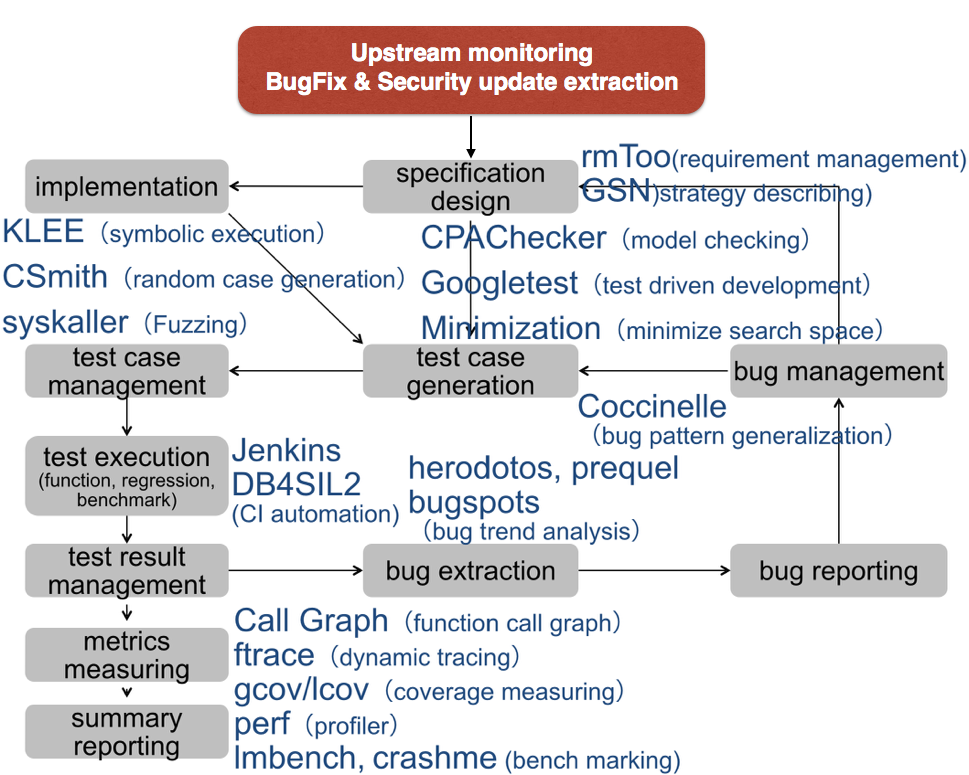
\includegraphics[width=\textwidth]{pic/safedist.eps}
  \caption{検証フレームワークの機能安全対応\acrshort{linux}ディストリビューションへの拡張}
  \label{safedist}
\end{figure}
\par
監視するべき\acrshort{oss}プロジェクトは多数存在するが、それらの開発基盤には事実上の世界標準であるバージョン管理システム\acrshort{git}が共通して使われている。
\acrshort{git}には全ての変更履歴がパッチとして記録されており、パッチにはそれぞれ変更の内容・意図・背景に関するコメントが付与されている。
アップストリームの監視と適用すべき変更の抽出を自動化するためには、\acrshort{git}パッチに含まれる情報を最大限利用する戦略が考えられる。
\pageref{presec}ページでは\acrshort{git}変更履歴に対してセマンティックパターンサーチを行うツール\acrshort{pre}を述べた。
\acrshort{pre}の戦略を拡張して、パッチコメントに対するセマンティックパターンサーチを行うことが出来れば
例えば特定のレベルのバグ修正やセキュリティ更新を効率よく抽出できる可能性がある。
その後の評価や適用判断は人の介在が必要であるものの、一連の活動の契機となるアップストリーム情報のインプットを自動化することで、
トレーサビリティの確保された属人的でないプロセス実現の足掛かりを得ることが期待される。
\par
その他、\acrshort{linux}システムのビルドフレームワークとして
\href{https://git.yoctoproject.org/cgit/cgit.cgi/}{\acrshort{yocto}} \cite{yocto}
が広く用いられている。
\acrshort{yocto}ビルドシステムは\acrshort{linux}ディストリビューションを構成する各\acrshort{oss}パッケージの
メタ情報(バージョン、適用パッチ、依存パッケージなど)から構成されており、
各々の\acrshort{oss}パッケージの更新状況は\acrshort{yocto}側のメタ情報にも随時活発に反映されている。
\acrshort{oss}アップストリーム情報をインプットする場所として、\acrshort{yocto}のような
\acrshort{oss}プロジェクト全体の情報が集まる場を上手に利用できれば、
重要なバグ修正やセキュリティ更新を迅速にキャッチしタイムリーに提供する体制を確立できると考えられる。
\par
本活動に対しては、機能安全対応の\acrshort{linux}ディストリビューションの構築と継続的メンテナンスサービス体制を確立することを目標に、
図\ref{safedist}に示したような「アップストリームの監視と適用すべき変更の抽出」をシスティマティックに実施する技法および方法論の調査と開発を行う。
\section{\acrshort{sil2linuxmp}コミュニティへの継続的なコントリビューション}
\pageref{contribution}ページで述べた目的の下、これまでと同様に以下の活動を今後も継続して行うことで機能安全に関するノウハウを蓄積し、
日立からの貢献を\acrshort{sil2linuxmp}コミュニティへアピールする。
\begin{enumerate}
  \item メーリングリスト上で質問や技術提案を行いコミュニティを巻き込んだ議論を行う。 \label{enum:ai1}
  \item ツール開発、実験・調査内容共有、ドキュメントレビューを\acrshort{git}上で行い貢献の記録を残す。 \label{enum:ai2}
  \item オンライン\acrshort{hazop}セッションへの参加または開催を行う。\label{enum:ai3}
\end{enumerate}
\ref{enum:ai2}.のツール開発、実験・調査内容共有は特に\acrshort{db4sil2}を対象とする。
現在\acrshort{db4sil2}はプロトタイプの段階であり技術調査・検討がさらに必要である。
特に、カバレッジ測定技法をユーザ空間にも拡張する具体的方法(\pageref{callgraph}ページ)、
コンパイラをT3ツールとして認証するために必要なエビデンスを得る方法論(\pageref{compveri}ページ)、
\acrshort{syzkaller}(\pageref{syzkaller}ページ)をはじめ\acrshort{fuzzer}として利用可能なツールの調査と\acrshort{db4sil2}への適用実験が今後の課題として挙げられる。
\par
また、\gls{agl}や\acrshort{genivi}などの団体が近年の機能安全対応の必要性から\acrshort{sil2linuxmp}プロジェクトの状況に関心を持っている。
今後は外部の\acrshort{oss}コミュニティに対して\acrshort{sil2linuxmp}の成果とノウハウを共有することが求められるため、
開発した検証技術と認証プロセスが現実のアプリケーションに即して適用できる形となることを確実にしていくことが必要である。

\chapter{現地の生活や文化の紹介}
本章ではインドでの生活や休日の旅行を通して思ったことを中心に記載する。
\section{平日の様子}
%\begin{wrapfigure}{r}{0.5\textwidth}
%\vspace*{-\intextsep}
%  \begin{center}
%    \includegraphics[width=0.5\textwidth]{pic/wtc.eps}
%    \caption{\acrshort{wtc}}
%    \label{wtc}
%  \end{center}
%\vspace*{-6\intextsep}
%\end{wrapfigure}
筆者が滞在したホテルは\acrshort{hil}オフィスが入居する\acrlong{wtc}から南に5km下った場所にあった。
\acrshort{wtc}とホテル間の移動にはホテル手配の車を利用した。
バスまたはメトロと徒歩で通勤することも可能であったが、\acrshort{hil}の方針で駐在員は研修員含めて仕事関係の移動は全て車を使うこととなっていた。
\acrshort{wtc}には\acrshort{ama}社のオフィスも入居しており、ホテルからの行き帰りの車で\acrshort{ama}社員と同乗することがよくあった。
話をすると、彼らは新しく\acrshort{ama}に採用されて一時的にホテルに滞在しているとのことである場合が多かった。
複数の\acrshort{ama}社員が同乗した場合は、おそらく機密事項に当たるであろうことを人のすぐ隣で大声で情報交換していた。
\par
出勤では当初ホテルを午前8時に出発していた。しかしある日突然\acrshort{wtc}へのメインロードが工事を開始したため通勤路を迂回しなければならなくなり、
ホテルを出る時間を早めなければならなくなった。
その工事は来る日も来る日も一切進んでいる気配がなく、遂に数ヶ月経って筆者が帰国する日になっても地面に大きな穴が空いたままであった。
\par
ホテルや\acrshort{wtc}、メトロの駅やショッピングモールの入り口では荷物検査と簡単なボディ検査が実施されている。
しかし職員の動きを見ている限りではそれはあくまでも形式上のもので、とても本当の危険物を発見できる体制には思えなかった。
建物内にはいたるところに警備員が配置されていた。
しかし一見過剰に思える人員配置や諸々の複雑な手続きも、それらの仕事によって雇用が確保されているので、無駄を省き全体の効率を図ろうとする力学がインド社会ではなかなか成立しないようである。
\par
\acrshort{hil}の終業時刻は午後5時であり、職場のほとんど全てのインド人が定時で帰宅していた。
筆者は日本にいた頃は慢性的に残業をしていたが、\acrshort{hil}は定時で帰るのが当たり前の環境であることと、ホテルの車に予め帰りの時間を指定していることで
筆者もほぼ定時で帰るようになった。
それに自然と仕事のリズムも合うようになり、定時でキリが良いように仕事が進むようになってそれで業務にも全く支障がなかった。
日本に帰っても無駄に残業せずに、基本的に定時で帰る前提で仕事を進めることを継続したい。
\begin{figure}[ht]
  \begin{minipage}{0.5\hsize}
  \begin{center}
    \includegraphics[width=\textwidth]{pic/wtc.eps}
  \end{center}
%   \caption{\acrshort{wtc}}
%   \label{orggraph}
  \end{minipage}
  \begin{minipage}{0.5\hsize}
  \begin{center}
    \includegraphics[width=\textwidth]{pic/cow.eps}
  \end{center}
%   \caption{適用後(85ノード、123エッジ)}
%   \label{minigraph}
  \end{minipage}
  \caption{\acrshort{wtc}とインドの道路。だいたい100m間隔で牛に遭遇する。}
  \label{wtc}
\end{figure}
%\begin{figure}[ht]
%  \centering
%  \includegraphics[width=0.7\textwidth]{pic/wtc.eps}
%  \caption{\acrlong{wtc}}
%  \label{wtc}
%\end{figure}
%\subsection{ホテル}
%\subsection{移動}
%\subsection{職場}
\section{週末の様子}
日本でやっていたテニスを継続したいと思いバンガロールで練習できる環境を探したところ、インド人ローカルのテニスクラブと日本人会のテニス部を見つけて毎週練習をしていた。
平日の移動手段が全て車であり日常生活で運動する機会がホテルのジム以外になかったため、週末のテニスは体力を維持するためにもとても助けになった。
ローカルのテニスクラブはコーチとの1対1レッスンで1時間Rs.600($\simeq$ \yen1000)と言われ、
インド人感覚からするとほぼぼったくり価格であったが、日本でスクールに通うよりはいくらか安いため
承知の上で月に一回くらい練習をさせてもらっていた。
コーチは毎週毎週「今週末は来るのか?」と電話をかけてくる非常に営業熱心な19歳の青年であった。
\par
日本人会テニス部では政府関係の人や企業の駐在員とその家族また学生までが一緒に練習していて、バンガロールに暮らしているたくさんの日本人と知り合うことができた。
活動場所はホテルから約4km離れた公園(Cubbon Park)内にある\acrshort{kslta}スタジアムであった。
ここではプロの試合も行われることがあり、2015年10月には\acrshort{kslta}で行われたATPチャレンジャーツアー男子ダブルスの決勝を観戦した。
練習日時は金曜日18:30-20:30と日曜日10:00-13:00であった。
夜に練習する場合は停電があると照明が復旧するまで15分ほど中断してしまうことや、コートが別の予定で突然使えなくなるなど、不便はあったものの
日本にいたときよりもはるかにたくさん練習を積むことができていろいろなショットが打てるようになった。
そのほかには平日の定時後にコンドミニアム敷地内にあるコートで練習することもあった。
\begin{figure}[ht]
  \begin{minipage}{0.5\hsize}
  \begin{center}
    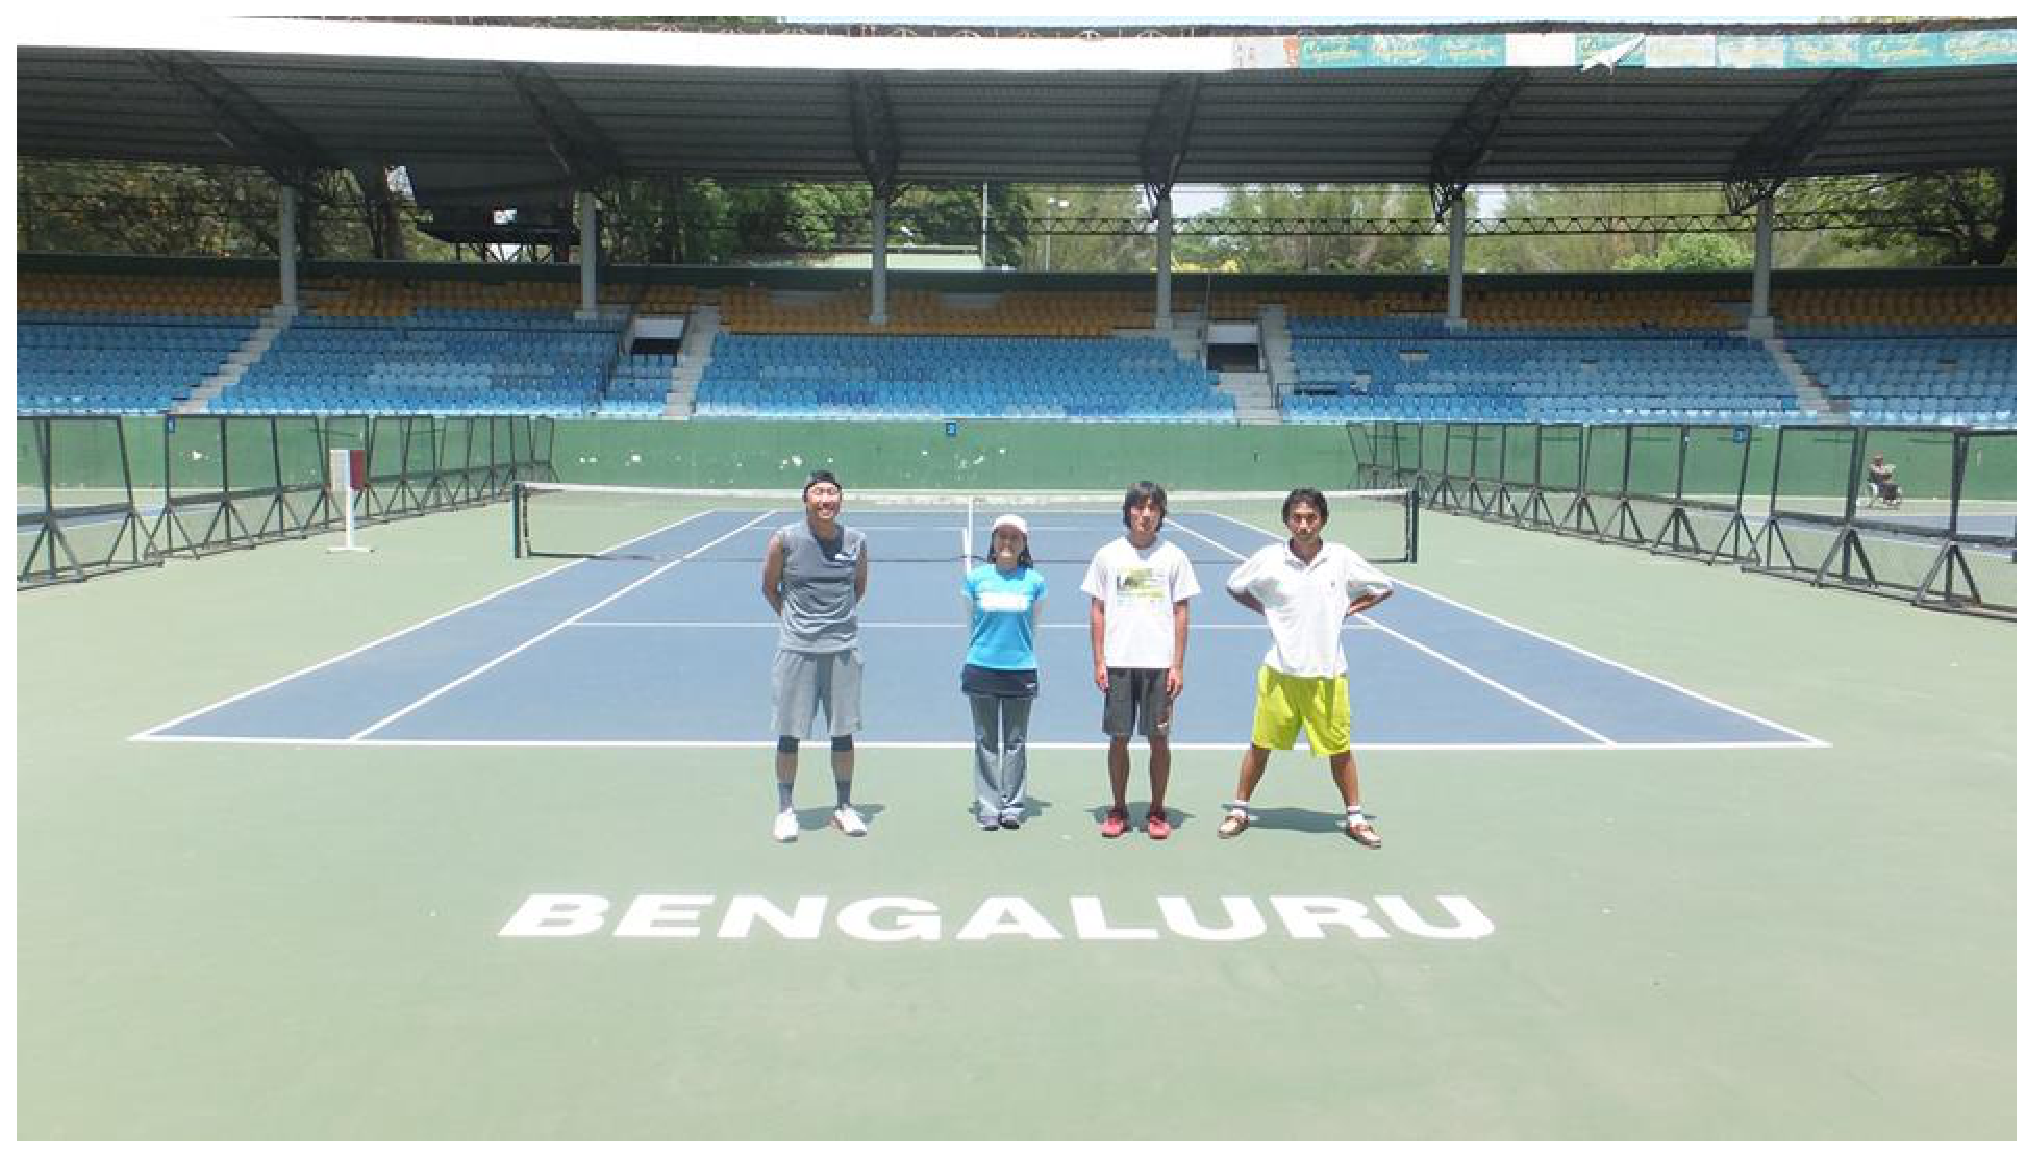
\includegraphics[width=\textwidth]{pic/kslta.eps}
  \end{center}
  \end{minipage}
  \begin{minipage}{0.5\hsize}
  \begin{center}
    \includegraphics[width=\textwidth]{pic/local.eps}
  \end{center}
  \end{minipage}
  \caption{\acrshort{kslta}スタジアムとインド人テニスクラブ。「今週は行けない」と言っても何度も電話してくる。}
  \label{wtc}
\end{figure}
\par
日曜日の夕方には\href{https://www.facebook.com/jinseidojo/timeline}{\acrlong{toast}} \cite{toast}に参加することがあった。
\acrshort{toastint} \cite{toastint}はパブリックスピーチや話し方の上達を目的とする国際的な団体で、バンガロールのコミュニティでは
日本語の勉強をしているインド人と英語の勉強をしている日本人が一緒に活動をしていた。
活動はバイリンガルで行われていて互いに言語の教え合いをすることもあった。
筆者は\acrshort{hil}の駐在員に紹介してもらって参加した。
即興で話題を振られて何かを話したり、即興で物語を作ったり、即興で他人のスピーチの論評したりと、とても頭を使う活動であった。
\begin{figure}[ht]
  \begin{minipage}{0.65\hsize}
  \begin{center}
    \includegraphics[width=\textwidth]{pic/toast1.eps}
  \end{center}
  \end{minipage}
  \begin{minipage}{0.35\hsize}
  \begin{center}
    \includegraphics[width=0.9\textwidth]{pic/toast2.eps}
  \end{center}
  \end{minipage}
  \caption{\acrshort{toast}バンガロールコミュニティ。筆者よりも日本語の語彙が豊富なインド人がいる。}
  \label{toast}
\end{figure}
\section{交通事情}
インドで暮らす上で、日本と全く異なるインドの交通事情に適応することは避けて通れない。
タクシーだけではなく様々な乗り物を使えるようになれば行動範囲と自由度がとても広がる。
本節では各交通手段別にそれぞれの特徴を述べる。
\subsection{バス}
筆者は休日に移動する際はほとんどバスを使用していた。
しかし筆者が聞いた限り、周りの日本人でバンガロールのバスに乗ったことのある人はいなかった。
それは、たくさんのバスが街中を走っている中で乗る場所や乗り方また行き先が分からないからである。
\acrshort{hil}のインド人に聞いてもバンガロールのバスは複雑でしかも不安定なので普通使わないと言っていた。
\par
バンガロールには100を超える数の路線バスが走っている。それぞれ、V-335EV, 258CC, KBS-3Eのような
数字とアルファベットの組み合わせが路線名としてバスの先頭に表示されている。
路線名の表示は手書きだったり、電光であっても消えていたり、現地語で書かれたりするため、まず路線名の視認が困難なことが多い。
路線名は走る地域や行き先によって似たような数字が割り当てられているようであるが、その規則性は全く不明である。
乗るべき路線名はGoogle Mapで行き先を調べることで分かるものの時間は全く当てにできない。
Google Mapでは通常複数の路線名が検索結果に出てくるので、それらを全てメモしておくとバスに乗れる確率が高まる。
なぜなら、Google Mapで示されたバス停に行っても狙った路線名のバスが一定時間内に来るとは限らないからである。
バス停といっても時刻表やバス停名などといった親切なものは一切なく、かろうじて屋根と椅子があることでバス停と分かるものとなっている。
目印が全くなく人が集まっているだけのバス停もある。
特に僻地のバス停ほどバスが来る頻度が低いため、乗ることのできる路線名をできる限り多く把握しておくことが必要となる。
筆者の場合はホテルから徒歩15分程度の場所にバンガロールシティ駅に隣接するバスターミナル(Kempegowda Bus Station)があったので、
バスの乗り降りはそのバスターミナルで行った。ここでは近辺の全ての路線が乗り入れるので、乗りたい路線にほぼ確実に一定時間内に乗ることができた。
\par
バスの料金は、乗ってからしばらくしてやってくる集金係に行き先を告げると金額を教えてくれるので手渡しで支払う。
親切な集金係だと伝えた場所に着くと知らせてくれる場合もあるが、基本的に自分で降りる場所を把握していなければならない。
気の利いた車内アナウンスなどはもちろんない。
料金は5km-15kmの道のりでだいたいRs.10-20($\simeq$ \yen15-30)と非常に安い。
ここでRs.50紙幣やRs.100紙幣を出すと受け取ってもらえないか非常に嫌がられるので、Rs.1やRs.10単位の細かい額を持っておかないと支払いに手間取ってしまう。
Rs.500紙幣やRs.1000紙幣などは言語道断である。どうしても集金係にお釣りがないときは、
「降りるときに何ルピー受け取る」というメモをその場で書いて渡してくれる。
もちろん申告しなかったり降りるときもお釣りがなかったりという場合はもらうことができない。
バスに限らず商店やモールでもみんなが細かいお金を欲しがるので、気をつけて小額紙幣や小銭を切らさないようにしていないとRs.500札やRs.1000札だけになってしまい
日常生活に支障をきたすことになる。
\par
バスには必ず運転手と集金係の必ず二人のスタッフがいる。
バスがどんなにぎゅうぎゅう詰めに混んでいても、集金係は新しく乗ってきた人を見失わずに人を押し退けバスの中を前に後ろに移動するのでとても大変である。
バスの中は前半分が女性で後半分が男性の空間という暗黙の了解があり、空いているからといって前に座ると注意される。
バスは走行中もドアが常に開きっぱなしで、ドアが壊れていることもよくある。バス車体の状態は整備という概念があるのか疑問に思うほどで、どのバスもひどい排気ガスを放出していた。
道路が平らでないことも相まって乗り心地は良いとは言えないが、タイミングよく乗ることができれば非常に安価で便利な移動手段である。
ただし道路が渋滞しているときは徒歩よりも遅い。
\begin{figure}[ht]
  \begin{minipage}{0.5\hsize}
  \begin{center}
    \includegraphics[width=\textwidth]{pic/busint.eps}
  \end{center}
  \end{minipage}
  \begin{minipage}{0.5\hsize}
  \begin{center}
    \includegraphics[width=\textwidth]{pic/kbs.eps}
  \end{center}
  \end{minipage}
  \caption{バンガロール市内の路線バス内とKempegowda Bus Station内の案内の一つ}
  \label{bus}
\end{figure}
\subsection{鉄道}
インドの鉄道には主に都市間や長距離を結ぶディーゼル機関車と、デリーなどの都市圏内で運行するメトロと言われる電車がある。
ここでは中長距離を結ぶ\acrlong{ir}について記載する。
筆者は週末や休日の旅行の際に\acrlong{ir}を利用した。インド滞在中に利用した区間は
Mumbai-Aurangabad間(約360km、8時間)、Bangalore-Mysore間(約140km、3時間)、Bangalore-Hospet間(約350km、8時間)
であった。
\acrlong{ir}を利用するためには座席の予約が必要であることになっている。
ただし後述するように事実上は予約せず運賃も払わずに乗車することは可能であるため、
無賃乗車で利用している客は一定数存在すると思われる。
筆者は\acrshort{maketrip}というインドの旅行手配サービス\cite{maketrip}を日本人会テニス部で教えてもらい、そこを介して\acrlong{ir}チケットの購入を行った。
駅の窓口で直接チケットを購入することもできるようであるが、\acrlong{ir}の座席予約システムが非常に複雑であることもあり
インド人と直接会話してチケットを確実に確保できる自信がなかったためweb上で予約を行った。
\par
\acrlong{ir}チケットを購入するためには、前提として\acrshort{wl}という\acrlong{ir}独自のシステムを理解する必要がある。
\acrlong{ir}にはこの複雑な\acrshort{wl}システムに起因する数々の独自のしきたりが存在しており、
特に旅行者が\acrlong{ir}を利用する際に混乱する要因となっている。
web上を検索するとこの\acrlong{ir}予約方法に関する\acrshort{wl}用語の質問や解説が山のように出てくるほか、
\href{http://trainstuff.in/}{\acrlong{ir}の利用方法ノウハウを第三者がまとめたサイト} \cite{trainstuff}
では\acrshort{wl}の仕組み解説のために特別にページを割いているほどである。
大前提として、\acrlong{ir}チケットは購入した時点で座席が確保されない。
座席数を超える予約が入っている場合であっても\acrlong{ir}予約システム上はチケットを購入できてしまうため、
それをもって実際に座席を確保できる条件を予め把握しておかないと、
予約が確定したと勘違いした結果当日になって列車に乗ることが出来ないということが起こり得る。
\par
用意された座席数が埋まっていない場合は座席の権利が確定したチケット(confirmed)を購入できるが、
既に埋まっている場合は\gls{rac}または\acrshort{wl}と呼ばれる区分のチケットを購入することになる。
\acrshort{rac}は「列車に乗車する権利があるが座席は保証しない」チケットである。
この場合は座席の権利を持った客が現れない場合そこに座るか、他の客の席を分けてもらうか、または立って乗車することになる。
confirmedチケットのキャンセルがあると随時先着順で\acrshort{rac}がconfirmedに繰り上がる。
confirmedと\acrshort{rac}で割当てられた分のチケットが売り切れると\acrshort{wl}チケットを購入することとなる。
\acrshort{wl}は座席の権利も乗車の権利もなにもなく、
confirmedチケットまたはRACチケットでキャンセルがあることを前提に権利が繰り上がることが期待できるのみである。
当日になっても\acrshort{wl}から繰り上がらなかった場合は料金が自動的に返金される。
\acrshort{rac}または\acrshort{wl}は購入する時点で何人たまっているのかが分かるようになっており、
購入した後もキャンセル状況によって自分がリストの何番目なのかの情報が\acrshort{maketrip}サイト上で随時更新されるため、
乗車・座席の権利が繰り上がる可能性をある程度予測することができる。
\acrshort{wl}チケットはさらに4種類ほどのタイプに区分されるがここではこれ以上の説明を省略する。
どの区分のチケットであっても期日前なら特にペナルティなくキャンセルが可能である。
ただし\acrshort{maketrip}や\acrlong{ir}のサイトは特に夜間不安定になる傾向があるため、
予約手続きが途中で失敗したりサイトが一時閉鎖していたりということに頻繁に遭遇する。
\acrshort{wl}の仕組みを理解し、かつ\acrshort{maketrip}上の手続きが成功して初めて何らかの乗車可能性が期待できるチケットを購入することができる。
\par
当日になってconfirmedチケットを手にしていた場合であっても座席の場所は
列車の発車時刻数時間前に用意されるChartを確認するまで把握することが出来ない。
Chartはその列車に乗車できる客の最終確定リストであって、乗車直前に\acrshort{maketrip}で確認するか、
駅の端末または張り出された紙で確認するか、各車両のドアに張り出された紙を確認する必要がある。
Chartには客の名前や性別年齢等の個人情報がプライバシー無関係に記載されている。
当日になってChartに自分の名前があることと座席番号が記載されていることを確認して初めて安心して列車に乗ることができる(図\ref{chart})。
\begin{figure}[ht]
  \centering
  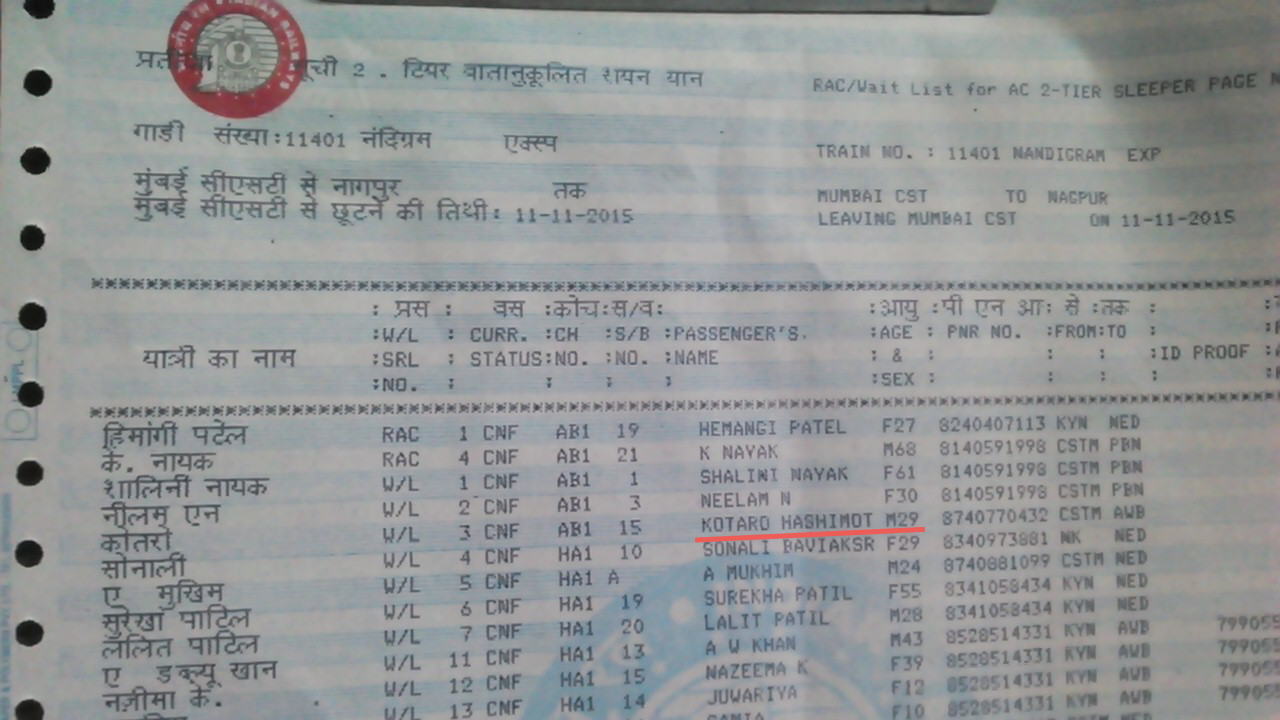
\includegraphics[width=\textwidth]{pic/chart.eps}
  \caption{列車の入り口に貼られているChartに自分の名前が確認できて安心しているところ}
  \label{chart}
\end{figure}
\par
このようなキャンセル待ち前提のシステムは旅行の計画を立てる上で大きな不安要素となるため、
筆者はconfirmedで取れるチケットを探して予約を行い、当日も無事にChartに名前を確認して座席を確保することができた。
しかし実際に乗車する現場では、特に下位クラスの車両では予約したはずの座席に既に人がいたり、網棚に人が登るほど乗車率が高かったり、特にチケットを確認されなかったりと、
複雑な予約システムに苦労して従う意味が本当にあったのか疑問である。
\begin{figure}[ht]
  \begin{minipage}{0.5\hsize}
  \begin{center}
    \includegraphics[width=\textwidth]{pic/train.eps}
  \end{center}
  \end{minipage}
  \begin{minipage}{0.5\hsize}
  \begin{center}
    \includegraphics[width=\textwidth]{pic/trainint.eps}
  \end{center}
  \end{minipage}
  \caption{Chartや予約システムなど関係なく大量に乗車するインド人}
  \label{railway}
\end{figure}
\par
ちなみにキャンセル前提でとりあえず予約するという文化は\acrshort{hil}内にも存在しており、\acrshort{hil}のミーティングルームの予約はほぼ全て常に誰かに押さえられていた。
実際は予約されたミーティングルームは使われていないことが多いため、予約システムの状況関係なく随時空いている部屋を探して利用することがほとんどであった。
\subsection{メトロ}
メトロは都市圏内で運行される電車である。
\acrlong{ir}の中長距離列車の場合では、だいたい常に30分くらい遅れて、走行中ドアが開きっぱなしで、停車の案内などが一切なく改札もない、
ということと比較するとメトロはきちんと管理されている。
利用する場合は、駅の窓口で行き先を告げてトークンと呼ばれる非接触ICタグを受け取る。料金はだいたい5kmでRs.15($\simeq$ \yen25)である。
プリペイドカードを持っていれば毎回窓口に行く必要がない。
メトロは分単位のスケジュールで運行されており本数も多く、インドでは時間が信頼できる唯一の交通手段である。日本の電車とほぼ相違ない。
\par
ただしバンガロールでは現在もメトロは建設中であって、部分的に完成している範囲しか運行していない。
数年単位の計画の遅れはインドでは特に気にしないようである。
全て完成するとバンガロール市内を中心に東西と南北に交差するようになり非常に便利になるが、筆者の滞在中は交差するところまではるかに届いていなかった。
メトロ一本で目的地に行けることはないため徒歩と組み合わせて利用していたが、朝夕の道路渋滞時にバスが当てにならないときなどは便利であった。
\begin{figure}[ht]
  \centering
  \includegraphics[width=0.7\textwidth]{pic/metro.eps}
  \caption{ショッピングモールが隣接するメトロ駅。ここから先の線路は工事中である。}
\end{figure}
\subsection{リキシャ}
リキシャはインド全国で見かける個人タクシー相当の三輪の乗り物で、「オート」や「トゥクトゥク」と言うこともある。
バンガロールでは四輪車のタクシーが走っていないため、現地の人も旅行者もリキシャを使う機会がとても多い。料金はだいたい路線バスの3-4倍程度である。
ただし、ドライバーによってはメーターを使わずに高い料金をふっかけてくることがある。
そういう場合は無理して交渉せずさっさと降りて別のリキシャに声をかければよい。
交渉を避けてスムーズにメーターを使ってもらうためには、現地の地理をよく知ってるフリをして目的地を口頭で伝えることが重要である。
ここで地図を出して行き先を伝えようとしてもリキシャのドライバーには地図が通用しない。
地図ではなく道路名や目印になる建物や場所を言うとスムーズである。
むしろ地図を出すと道や相場を知らない観光客と思われてカモにされる。
後々の面倒を避けようと乗るときに「ここまでいくらか」と聞くのも、メーターを知らない観光客と思われて自分からぼったくられに行くようなものなので、
メーターを使ってくれるように自然に振舞うことが重要である。
あっさりメーターを使ってくれない場合は遠慮せず降りて他のリキシャを探せばよい。
\begin{figure}[ht]
  \centering
  \includegraphics[width=0.7\textwidth]{pic/rikisya.eps}
  \caption{インド全国で気軽に乗れるリキシャ。上半分が黄色で下が緑か黒のデザイン。}
\end{figure}
\subsection{タクシー}
インドでは流しのタクシーが走っていない。
タクシーを使う場面はホテル手配の車で通勤するときと職場手配の車でどこかに出かける場合のみであった。
タクシーを使う場合はドライバーに時間と場所を毎回指定する必要がある。
職場から帰るときも\acrshort{wtc}に来て欲しい時間を毎回伝えていたが、時間通りに来てくれる確率は非常に低かった。
インドでは日本と異なり時間が正確に守られない事象に頻繁に遭遇する。一部のインド人はそもそも
人を待たせることを悪いと思っていないように見受けられるので、それでいちいち怒らずにうまくイナす心がけが重要である。
しかし、毎日事前に時間を伝えて来てもらうことと、伝えた時間に来ないことを考えると、
移動のためにそのような不確実で手続きが面倒なインフラに頼らざるを得ないことが非常に不自由に感じるようになった。
\subsection{徒歩}
以上の交通事情を総合すると、渋滞や時間・人の不確実さに依存しない移動手段として、徒歩が最も楽で確実で自由度が高いと思うようになった。
そのため、5km程度の移動では特にバスを調べずに歩くようになった。
再度インドに長期滞在することがあったらこんどは移動を自己完結できるように自転車を用意したい。
ただし自転車が盗まれないための何らかの対策は必要である。
また、バスやリキシャが出す排気ガス対策としてマスクも必須である。
インドでは自転車は貧困層の乗り物という意識があると聞いたことがあるが、
バンガロールでは自転車に乗る人はほとんど見かけなかった。
\par
バンガロールの道路は一日中常にクラクションの音であふれている。
\acrshort{hil}通勤時の車でのドライバーの動きを見ている限り、クラクションは危ないときに鳴らすのではなく
「通りますよ」の意味で自分の存在を知らせるために鳴らすらしい。
日本ではクラクションの意味が重いため鳴らすのに一定の心理的ハードルがあるが、
インドでは追い越しするときや細い道に入るときや人のそばを通るときなど非常に気軽にクラクションが鳴らされる。
大きなトラックの後ろにはわざわざ"Sound Horn"と書かれており、鳴らされる方もクラクションを期待しているようである。
おそらくインドの道を自転車で走るとなると追い越されるたびにクラクションを鳴らされてびっくりすることになるが、
それは別に危ないと怒られているわけではないので、クラクションをいちいち気にしない強いメンタルを身につける必要がある。
\section{旅行}
研修期間中は休日や週末を利用して南インド中心に旅行に出かけた。
年末年始はスリランカの街と遺跡を巡り、3月にはドイツに出張しハイデルベルグの街を観光した。
\begin{figure}[ht]
  \centering
  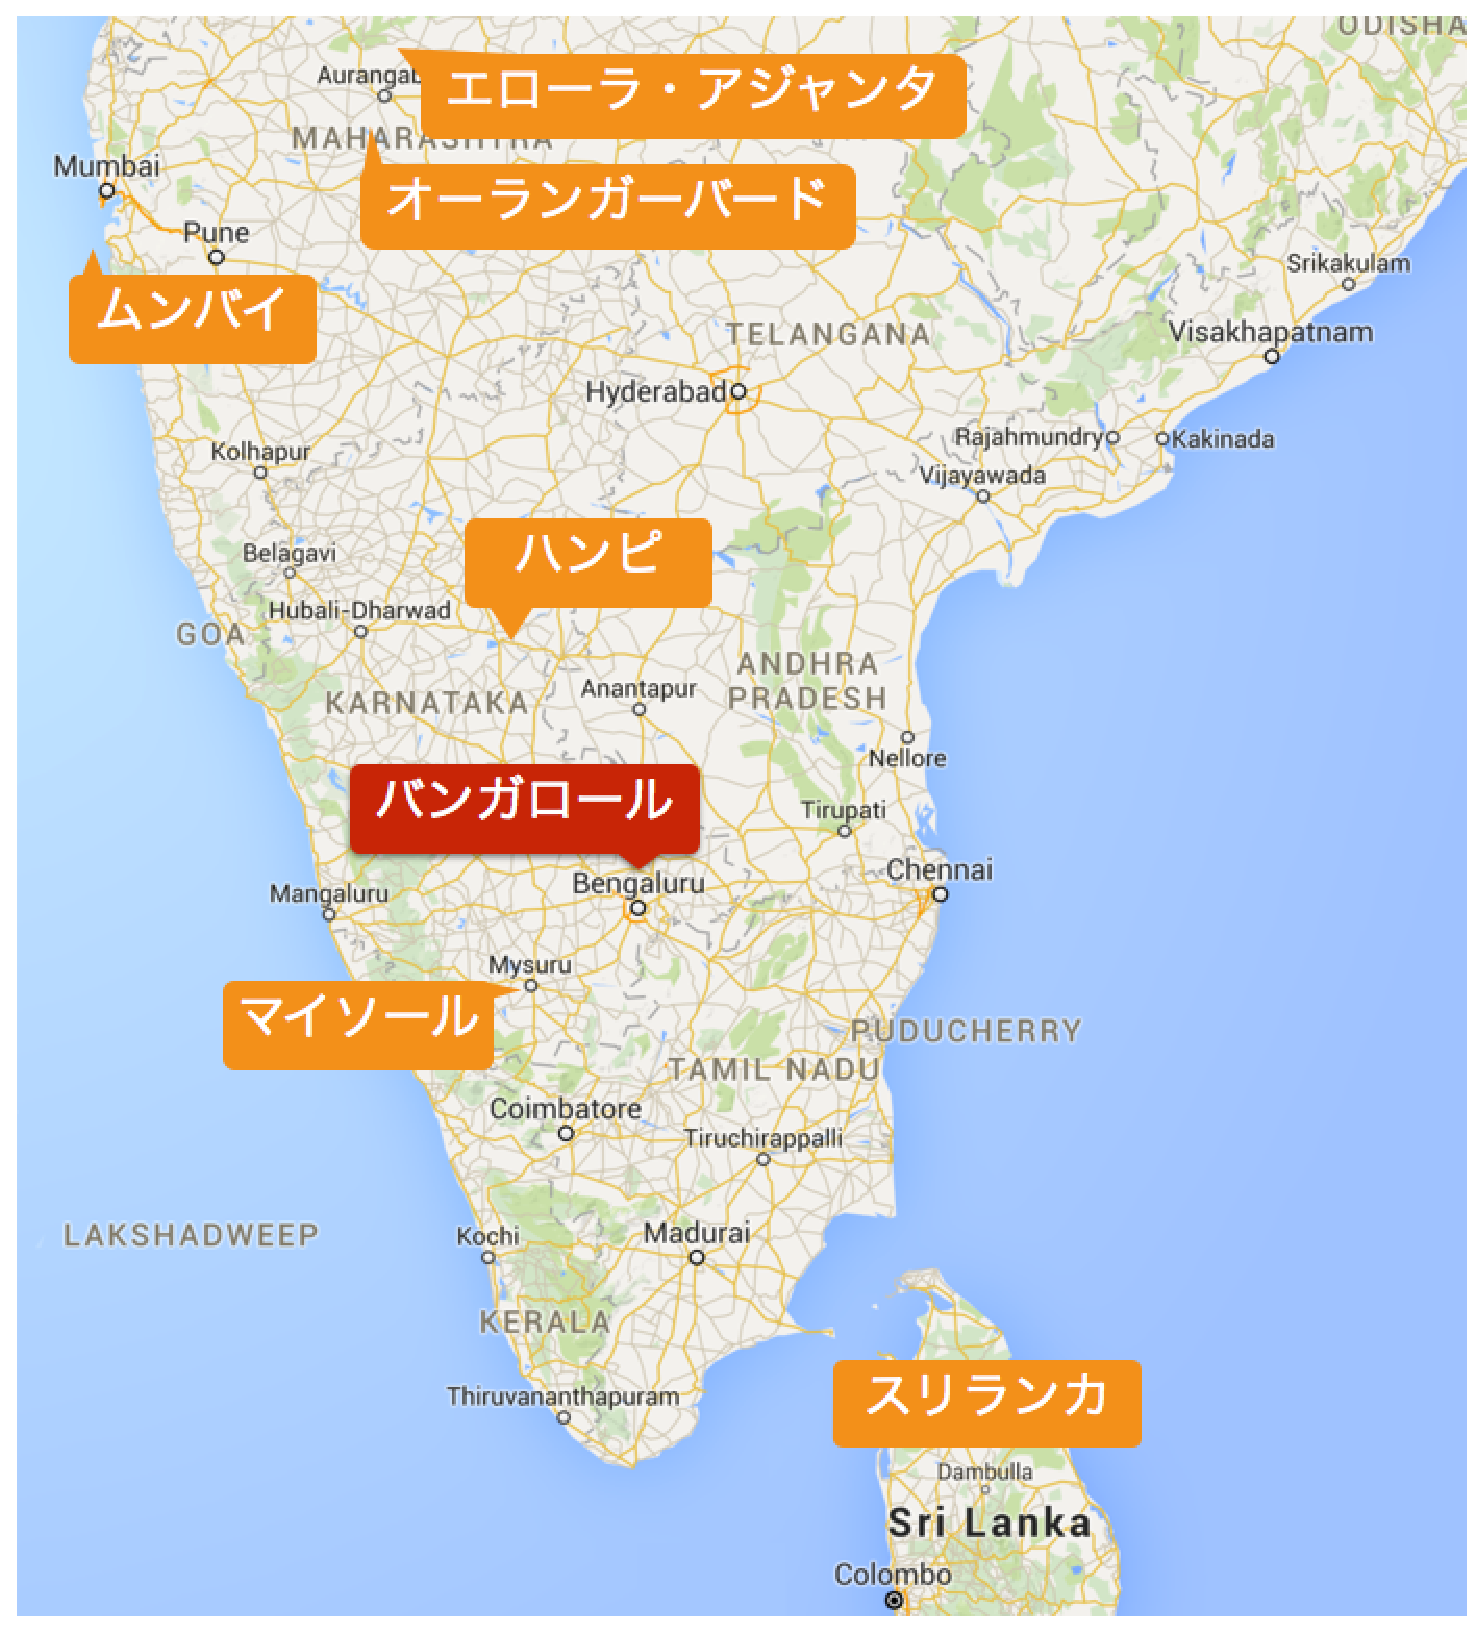
\includegraphics[width=0.9\textwidth]{pic/india.eps}
  \caption{研修期間中に訪れた南インド周辺の地域}
\end{figure}
\subsection{ムンバイ、オーランガーバード、エローラ・アジャンタ}
11月中頃にDiwaliというインドの祭典があり、それに伴い5日間の連休を取得して世界遺産に登録されているエローラ石窟群とアジャンター石窟群を訪れた。
バンガロールから飛行機でムンバイまで行き、ムンバイ市内をローカル鉄道で移動し、ムンバイからオーランガーバードまで7時間の長距離列車に乗り、
オーランガーバードからエローラとアジャンターまでは長距離バスを使った。
旅行の目的の半分以上が、インド国内の特に初めての鉄道での移動に挑戦することであった。
先述した通りインドの鉄道は乗り方が複雑なため、移動中に迷ったり乗り換えを間違えたりしても大丈夫なようにかなり余裕をもったスケジュールを組んだが、しかし実際は拍子抜けするくらい予定通りに移動ができてしまった。
ムンバイの空港から鉄道のターミナル駅に行く途中では乗り合わせた現地人が付き添って乗り換えの仕方まで教えてくれた。
特にそれでチップを求められるわけでもなかった。
オーランガーバードへ向かう長距離列車では互いに口の訊けない子連れの夫婦と相席になり、長距離バスでは高校生達と連絡先を交換し、
アジャンターで一泊したときはたまたま知り合った現地の人に家と街を案内してもらい、
そのほか行く先々でたくさんの現地の人との出会いがあってその度に何かと助けてもらった。
\begin{figure}[H]
  \begin{minipage}{0.5\hsize}
  \begin{center}
    \includegraphics[width=\textwidth]{pic/cst.eps}
  \end{center}
  \caption{ムンバイの世界遺産であり現役ターミナル駅のChhatrapati Shivaji Terminus}
  \end{minipage}
  \begin{minipage}{0.5\hsize}
  \begin{center}
    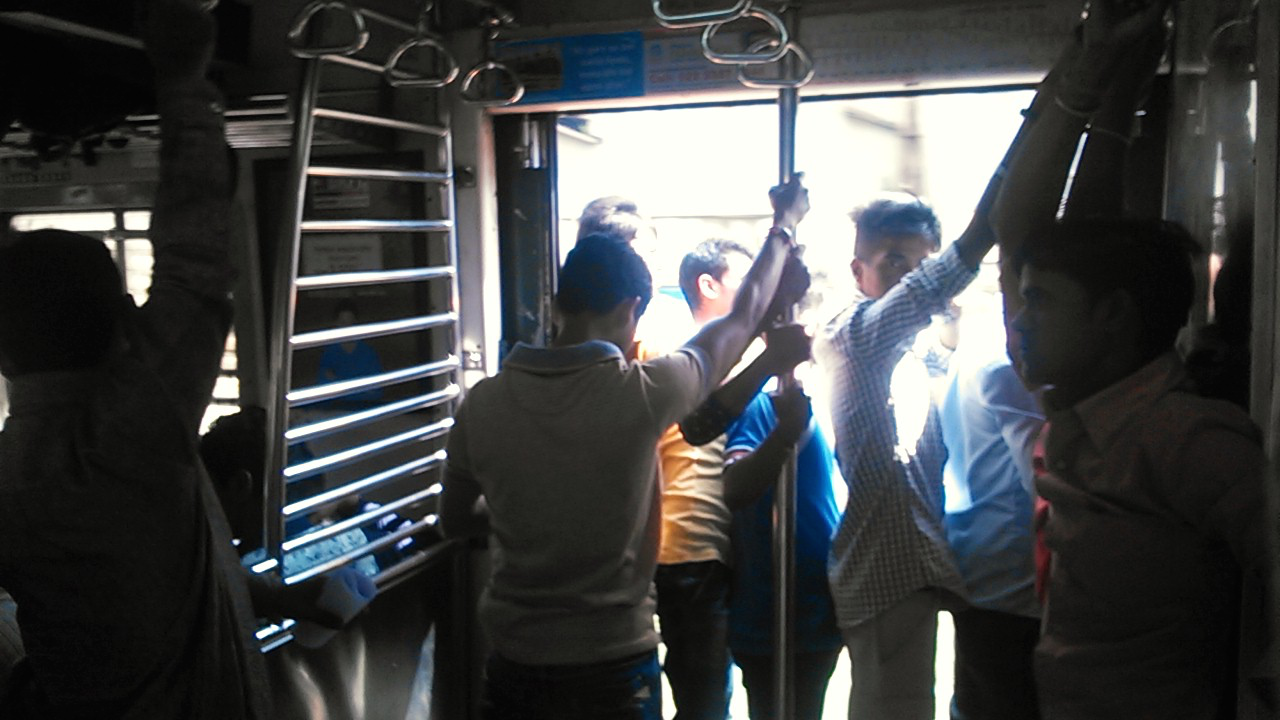
\includegraphics[width=\textwidth]{pic/mumbaitrain.eps}
  \end{center}
  \caption{ムンバイ市内の鉄道。走行中も開きっぱなしのドアから身を乗り出している人が多い。}
  \end{minipage}
\end{figure}
\begin{figure}[H]
  \begin{minipage}{0.5\hsize}
  \begin{center}
    \includegraphics[width=\textwidth]{pic/auranbus.eps}
  \end{center}
  \caption{オーランガーバードのバスターミナル。世界的な遺跡への拠点なのに英語の案内がない。}
  \end{minipage}
  \begin{minipage}{0.5\hsize}
  \begin{center}
    \includegraphics[width=\textwidth]{pic/uso.eps}
  \end{center}
  \caption{タージマハルによく似たBibi Ka Maqbara。行く先々で現地人に写真をせがまれる。}
  \end{minipage}
\end{figure}
\begin{figure}[H]
  \begin{minipage}{0.39\hsize}
  \begin{center}
    \includegraphics[width=\textwidth]{pic/diwalipic.eps}
  \end{center}
  \caption{Diwali期間中に民家の玄関口に描かれる装飾}
  \end{minipage}
  \begin{minipage}{0.39\hsize}
  \begin{center}
    \includegraphics[width=\textwidth]{pic/shonen.eps}
  \end{center}
  \caption{アジャンター石窟群に隣接する街Fardapurを案内してくれた青年}
  \end{minipage}
  \begin{minipage}{0.19\hsize}
  \begin{center}
    \includegraphics[width=\textwidth]{pic/furadapura.eps}
  \end{center}
  \caption{Fardapur青年の家と家族}
  \end{minipage}
\end{figure}
\begin{figure}[H]
  \begin{minipage}{0.5\hsize}
  \begin{center}
    \includegraphics[width=\textwidth]{pic/kago.eps}
  \end{center}
  \caption{アジャンター石窟群での「椅子」客待ち}
  \end{minipage}
  \begin{minipage}{0.5\hsize}
  \begin{center}
    \includegraphics[width=\textwidth]{pic/vendor.eps}
  \end{center}
  \caption{駅に止まるたびに売り子がやってくる}
  \end{minipage}
\end{figure}
\subsection{マイソール}
マイソールはかつてマイソール王国の首都として栄えた文化的歴史がある都市である。
バンガロールから日帰りで片道約3時間かけて鉄道で移動し、マイソール宮殿やマーケットを見て歩いた。
マーケットでは大量の生花、野菜、果物(ほとんどバナナ)、粉、布、香辛料、茶、葉っぱ、草、人の髪などが取引されており、
何のためにどうやって使うのかが分からないものが多かった。
\begin{figure}[H]
  \begin{minipage}{0.5\hsize}
  \begin{center}
    \includegraphics[width=\textwidth]{pic/market.eps}
  \end{center}
  \caption{マイソールのDevaraja Market}
  \end{minipage}
  \begin{minipage}{0.5\hsize}
  \begin{center}
    \includegraphics[width=\textwidth]{pic/kona.eps}
  \end{center}
  \caption{DiwaliやHoliの祭典で使われる粉}
  \end{minipage}
\end{figure}
\subsection{ハンピ}
ハンピはカルナータカ州北部にある都市遺跡である。
あまり観光地されておらず、中心部であってもごく小さなバザールや安宿街があるだけのとても静かな場所であった。
バンガロールからは約8時間の寝台列車でホスペットまで移動し、そこから約1時間のバスで行くことができる。
観光客にはインド人のほか欧米人が多かった。
訪れた時期が3月下旬でちょうどインドの祭典Holiの時期だったため、顔や体にカラフルな粉や液体をかけた(かけられた)人をたくさん見た。
バザールを歩いていて突然筆者のすぐ後ろで現地の子供に色水をかけられた観光客がいたが、筆者は防水対策をしていなかったためすぐに逃げた。
ハンピには広い範囲に遺跡が点在していて、地域全体に奇妙な形の岩が奇妙な構成で積み上げられている。
人工物なのか自然現象の結果なのか分からないものが多く、
いったい何がどうなればあのような岩の構成物ができるのか全く理解できなかった。
\begin{figure}[H]
  \begin{minipage}{0.5\hsize}
  \begin{center}
    \includegraphics[width=\textwidth]{pic/rock1.eps}
  \end{center}
  \caption{ハンピで唯一遺跡にならずに現役で活動し続ける寺院Virupaksha Temple}
  \end{minipage}
  \begin{minipage}{0.5\hsize}
  \begin{center}
    \includegraphics[width=\textwidth]{pic/hill.eps}
  \end{center}
  \caption{Matanga Hillからの風景。ここで昼寝した。}
  \end{minipage}
\end{figure}
\begin{figure}[H]
  \begin{minipage}{0.5\hsize}
  \begin{center}
    \includegraphics[width=\textwidth]{pic/hampipp.eps}
  \end{center}
  \caption{遺跡でピクニックをするインド人}
  \end{minipage}
  \begin{minipage}{0.5\hsize}
  \begin{center}
    \includegraphics[width=\textwidth]{pic/hampi.eps}
  \end{center}
  \caption{喜んで写真に応じてくれるが一回Rs.100}
  \end{minipage}
\end{figure}
\begin{figure}[H]
  \begin{minipage}{0.5\hsize}
  \begin{center}
    \includegraphics[width=\textwidth]{pic/hampi2.eps}
  \end{center}
  \caption{Holiを祝うHampiの子供}
  \end{minipage}
  \begin{minipage}{0.5\hsize}
  \begin{center}
    \includegraphics[width=\textwidth]{pic/dog.eps}
  \end{center}
  \caption{Holiされた犬}
  \end{minipage}
\end{figure}
\subsection{スリランカ}
スリランカはインドのすぐ南に位置しており、バンガロールから気軽に気軽に行くことができる。
スリランカ旅行を計画した当初はアーユルヴェーダ施設に一週間入ることを考えていたが、スリランカは初めてだったため
王道の遺跡・寺院巡りをすることとした。
バンガロールからネゴンボまでは飛行機で行き、そこから各都市への移動には鉄道と長距離バスを利用した。
スリランカの鉄道システムは\acrlong{ir}のように複雑でないので、特に予約せずとも問題なく現地でチケットを購入できる。
ちなみにインドの隣国であるにもかかわらずスリランカの空港(Bandaranaike)ではインドルピーの両替ができない。
これはインドルピーが国外持出し禁止とされているからであるが、タイ、シンガポール、マレーシアなどで
インド人の移民が多く集まる地域では両替が可能な場所が存在するらしい。
スリランカでも探せばコロンボでインドルピーを受け付けてくれる両替商があるかもしれない。
\begin{figure}[ht]
  \centering
  \includegraphics[width=0.9\textwidth]{pic/srilanka.eps}
  \caption{年末年始に訪れたスリランカの地域}
\end{figure}
\begin{figure}[H]
  \begin{minipage}{0.5\hsize}
  \begin{center}
    \includegraphics[width=\textwidth]{pic/fort.eps}
  \end{center}
  \caption{コロンボから各都市への起点となるFort駅}
  \end{minipage}
  \begin{minipage}{0.5\hsize}
  \begin{center}
    \includegraphics[width=\textwidth]{pic/sritrain.eps}
  \end{center}
  \caption{アヌラーダプラに到着したところ}
  \end{minipage}
\end{figure}
\begin{figure}[H]
  \begin{minipage}{0.5\hsize}
  \begin{center}
    \includegraphics[width=\textwidth]{pic/interbus.eps}
  \end{center}
  \caption{都市間を結ぶバス。本数が多くて便利。}
  \end{minipage}
  \begin{minipage}{0.5\hsize}
  \begin{center}
    \includegraphics[width=\textwidth]{pic/alpine.eps}
  \end{center}
  \caption{売りに出されているトゥクトゥク。Alpine社との関係は不明。}
  \end{minipage}
\end{figure}
\begin{figure}[H]
  \begin{minipage}{0.5\hsize}
  \begin{center}
    \includegraphics[width=\textwidth]{pic/ajinomoto.eps}
  \end{center}
  \caption{どこにでも必ず置いてあるAJINOMOTO}
  \end{minipage}
  \begin{minipage}{0.5\hsize}
  \begin{center}
    \includegraphics[width=\textwidth]{pic/monkey.eps}
  \end{center}
  \caption{ポロンナルワ遺跡群に住み着いている猿}
  \end{minipage}
\end{figure}
\begin{figure}[H]
  \begin{minipage}{0.5\hsize}
  \begin{center}
    \includegraphics[width=\textwidth]{pic/pond.eps}
  \end{center}
  \end{minipage}
  \begin{minipage}{0.5\hsize}
  \begin{center}
    \includegraphics[width=\textwidth]{pic/tooth.eps}
  \end{center}
  \end{minipage}
  \caption{キャンディ仏歯寺とその隣の池}
\end{figure}
スリランカはインドと比べると道が綺麗で、また旅行者に対して優しいという印象を持った。
現地に行っても必要な情報がきちんと英語で表示されていて、迷っていたら誰かがすぐに声をかけてくれて、かといって客引きがしつこいわけでもなく、
旅の難易度はインドよりも低いと感じた。
インドとは地理的に近く文化も似ている点が多いが、国教が仏教であるため遺跡や寺院では仏像を多く見る。
\begin{figure}[H]
  \begin{minipage}{0.33\hsize}
  \begin{center}
    \includegraphics[width=\textwidth]{pic/bicycle.eps}
  \end{center}
  \caption{ゲストハウスで借りた自転車が日本の寄付物のようで「阿倍野郵便局」と書いてあった}
  \end{minipage}
  \begin{minipage}{0.33\hsize}
  \begin{center}
    \includegraphics[width=\textwidth]{pic/sigiriya.eps}
  \end{center}
  \caption{高さ200mのシギリヤロック}
  \end{minipage}
  \begin{minipage}{0.33\hsize}
  \begin{center}
    \includegraphics[width=\textwidth]{pic/hasu.eps}
  \end{center}
  \caption{寺院の隣で売られているハスの花}
  \end{minipage}
\end{figure}
\subsection{ドイツ}
3月第一週に\acrshort{sil2linuxmp}マイルストンミーティングがドイツ・ハイデルベルグで行われた。
バンガロールからはフランクフルトまで直行便を使い、フランクフルトからハイデルベルグまでシャトルバスで移動した。
この時期のドイツはバンガロールと30℃以上の気温差があったが、インドには半袖と薄い服しか持ってこなかったためそのままの格好で行ったところ
フランクフルト空港は雪が降っていてとても寒かった。
\acrshort{sil2linuxmp}ミーティング終了後に参加者数人でハイデルベルグ城とOld Townの観光に行った際、
同行した人があまりに寒そうだと服を貸してくれた。
ハイデルベルグの古い街並みはとても美しく機能的だという印象を持った。
鉄道とトラム網がとても発達していて、道路は自転車が快適に走れるよう整備されていた。
\begin{figure}[H]
  \begin{minipage}{0.5\hsize}
  \begin{center}
    \includegraphics[width=\textwidth]{pic/tram.eps}
  \end{center}
  \caption{ハイデルベルグ街中を走るトラム}
  \end{minipage}
  \begin{minipage}{0.5\hsize}
  \begin{center}
    \includegraphics[width=\textwidth]{pic/heldel5.eps}
  \end{center}
  \caption{\acrshort{sil2linuxmp}ミーティング会場}
  \end{minipage}
\end{figure}
\begin{figure}[H]
  \begin{minipage}{0.5\hsize}
  \begin{center}
    \includegraphics[width=\textwidth]{pic/castle.eps}
  \end{center}
  \end{minipage}
  \begin{minipage}{0.5\hsize}
  \begin{center}
    \includegraphics[width=\textwidth]{pic/heldel6.eps}
  \end{center}
  \end{minipage}
  \caption{ハイデルベルグ城とそこから見下ろすOld Town}
\end{figure}
\section{食事}
インドではほとんど毎日果物を食べて生きていた。
あまり外の屋台で食べ物を買うなどのリスクを冒さなかったので、日本に帰るまで体調を崩すことはなかった。
筆者は日本では朝1リットルくらいブラックコーヒーを飲む。
しかしインドではブラックコーヒーを飲む習慣がなく、ホテルでもコーヒーはミルク入りで用意されている。
そのため毎朝ブラックコーヒーをオーダーしていた。
外国人も泊まるホテルで他にもブラックコーヒーをオーダーする人は多くいたにもかかわらず、
わざわざオーダーしないと用意してくれないシステムが改善される気配は遂になかった。
インド人は大半がベジタリアンであるため肉や魚を使ったメニューが少ない。
提供される肉も一般的な店やホテルではチキンのみである。
牛肉や豚肉を提供する店もバンガロール市内にないことはないがごく限られている。
ホテルでは毎日野菜がたっぷり朝食に並んでおり、半年間野菜と果物を主食としていたため日本にいたときよりも食生活は健康的であった。
日本でいうカレーに相当するものはあまり口にしなかった。
インド料理のことはよく分からないが、インドはカレーと一括りで言うことが失礼なほど多様なカレーのようなものがある。
むしろだいたい何を食べても固形物でも液体でもカレーのような味のするスパイスが効いているため、おそらくインドはカレーという区別がないのではないかと思う。
もちろん日本で食べるカレーの味をインドで求めるならば日本食レストランに行かなければならない。行ってもあるかどうかは分からない。
%\par
研修期間の後半になるにつれて、日本に帰ったら白米と海鮮物をとても食べたいと思うようになった。
\section{英語}
インド人の英語は聞き取りづらいというステレオタイプがあるが、発音は人それぞれである。
初めは聞き取りづらい人であっても耳が慣れれば問題なく意思疎通できるようになる。
\acrshort{hil}で働いていたインド人は英語のネイティブと遜色ないほど聞き取りやすく流暢な発音をする人が多かった。
筆者と一緒に仕事をしていたKrishnajiさん、Geetさんはそれぞれアメリカ、イギリスでの長期滞在経験があるとのことであった。
オフィスの外ではリキシャの運転手や特に地方に旅行に出かけたときに英語が通じにくいことがあった。
筆者は口頭でも文面でも結論や要点を先に伝えることを意識し、特に文法が正しくなくてもキーワードとなる単語を先に言うことを重視していた。
\par
バンガロールで耳にするまたは目にすることの多かった特徴的な英語表現としては、「営業時間」や「都合の良い時間帯」を意味するときに"timing"と言う
ことや、文中で重複を避ける際の代名詞に"the same"を使うことや、特にインド人同士の会話で"$\sim$, right ?"のようなニュアンスで"$\sim$, ノゥ ?"
と言うものがあった。
%\section{インド人}
%predictableであることがホッとする。
%時間に厳密でない。が人による。
%人を待たせることをそもそも悪いと思わない
%一番使う時間にトイレ掃除をしている
%昼のご飯を買うのに10分くらいかかる
%昼に戻ってこない。
%サービス、人が基本的に信頼できない。
%携帯電話の料金が払えない。
%電車予約システムが頻繁に落ちる。
%性悪説
\chapter*{謝辞}
\addcontentsline{toc}{chapter}{謝辞}
海外業務研修を実施するにあたり非常に多くの人に手厚いサポートをしていただきました。
派遣を推薦してくださった上長と研修を後押ししていただいた職場の皆様、
渡航前の準備から帰国後まで全面的に手続きを手伝っていただいた総務、
派遣を受け入れていただき現地の生活をサポートしてくださった\acrshort{hil}の皆様、
共に\acrshort{sil2linuxmp}プロジェクトに取り組んでいる研究所と\acrshort{hil}のメンバ、\acrshort{osadl}, \acrshort{ot}の技術者、
毎日職場まで運転してくれたドライバーと日々の生活の面倒を見てくれたホテルのスタッフ、
楽しい休日の思い出を作ってくれた日本人会テニス部と\acrshort{toast}、
旅先でフレンドリーに接してくれていろいろ助けてもらった見ず知らずの現地の人々、
非常に多くの人のサポートがあってこの業務研修ができたことを感謝しています。
今後も継続して\acrshort{sil2linuxmp}プロジェクトに取り組み、オープンソースソフトウェアの機能安全対応プロセス研究と
品質保証ノウハウ蓄積を進めます。
特に成果を\acrshort{hiics}のビジネスに展開することを念頭に置いて、引き続き\acrshort{sil2linuxmp}コミュニティと協力していく所存です。
\newline
\begin{figure}[ht]
  \centering
  \includegraphics[width=\textwidth]{pic/thanks.eps}
  \caption{\acrshort{hil}で一緒に仕事をしたチーム}
\end{figure}


%\appendix
%
%\include{appendixA}
%\include{appendixB}
%
%
%
%
%\include{biblography}
\bibliographystyle{jplain}
\bibliography{report}
%
%
%\newpage
%\printindex
%\chapter*{用語}
%\addcontentsline{toc}{chapter}{用語}
%\clearpage
%\printglossary[type=\acronymtype]
%\printglossary[type=\acronymtype]
%\printglossaries
%\printglossaries
%
%
\end{document}
